% Biên dịch bằng XeLaTeX (Overleaf: Menu > Compiler > XeLaTeX) hoặc Tectonic:  tectonic report.tex
% Trình bày theo quy định bài tập lớn của Trường Đại học Đại Nam: A4, Times New Roman 13, giãn dòng 1,5,
% lề trên 2 cm, lề dưới 2 cm, lề trái 2,5 cm, lề phải 2 cm, số trang ở giữa phía dưới.
\documentclass[a4paper,oneside]{report}
\usepackage[fontsize=13pt]{scrextend}

% ---------- Phông chữ: Times New Roman (nếu máy có), nếu không dùng TeX Gyre Termes (bản tương đương) ----------
\usepackage{fontspec}
\IfFontExistsTF{Times New Roman}{%
  \setmainfont{Times New Roman}%
}{%
  \setmainfont{texgyretermes}[Extension=.otf, UprightFont=*-regular, BoldFont=*-bold,
    ItalicFont=*-italic, BoldItalicFont=*-bolditalic]%
}
\setmonofont{texgyrecursor}[Extension=.otf, UprightFont=*-regular, BoldFont=*-bold,
  ItalicFont=*-italic, BoldItalicFont=*-bolditalic, Scale=0.85]

% ---------- Trang, dòng, đoạn ----------
\usepackage[a4paper, top=2cm, bottom=2cm, left=2.5cm, right=2cm, footskip=1cm]{geometry}
\linespread{1.44}   % tương đương giãn dòng 1,5 lines của Word với cỡ chữ 13
\setlength{\parindent}{1cm}
\setlength{\parskip}{6pt}
\usepackage{indentfirst}
\usepackage{microtype}

\usepackage{amsmath, amssymb}
\usepackage{graphicx}
\usepackage{booktabs, array, tabularx, multirow, makecell}
\usepackage{xcolor}
\usepackage{float}
\usepackage{etoolbox}
\usepackage{caption}
\DeclareCaptionFont{twelve}{\fontsize{12}{15}\selectfont}
\captionsetup{font={twelve,it}, labelfont={twelve,it}, labelsep=period, skip=6pt}
\usepackage{subcaption}
\captionsetup[sub]{font={twelve,it}, labelfont={twelve,it}}
\AtBeginEnvironment{table}{\fontsize{12}{15}\selectfont}
\usepackage{listings}
\usepackage{enumitem}
\usepackage{needspace}
\usepackage{tikz}
\usetikzlibrary{positioning, arrows.meta}
\usepackage{titlesec}
\usepackage{tocloft}
\usepackage{xurl}
\usepackage[hidelinks]{hyperref}

% ---------- Tên gọi tiếng Việt ----------
\renewcommand{\contentsname}{MỤC LỤC}
\renewcommand{\listfigurename}{MỤC LỤC HÌNH ẢNH}
\renewcommand{\listtablename}{MỤC LỤC BẢNG}
\renewcommand{\bibname}{DANH MỤC TÀI LIỆU THAM KHẢO}
\renewcommand{\chaptername}{Chương}
\renewcommand{\appendixname}{Phụ lục}
\renewcommand{\figurename}{Hình}
\renewcommand{\tablename}{Bảng}
\renewcommand{\lstlistingname}{Đoạn mã}

% ---------- Đề mục: tên chương 14 in hoa đậm giữa; mức 1: 13 đậm trái; mức 2: 13 đậm nghiêng trái ----------
\titleformat{\chapter}[block]{\centering\bfseries\fontsize{14}{20}\selectfont}
  {\MakeUppercase{\chaptertitlename}\ \thechapter.}{0.4em}{}
\titleformat{name=\chapter, numberless}[block]{\centering\bfseries\fontsize{14}{20}\selectfont}{}{0pt}{}
\titlespacing*{\chapter}{0pt}{0pt}{18pt}
\titleformat{\section}{\bfseries}{\thesection.}{0.5em}{}
\titleformat{\subsection}{\bfseries\itshape}{\thesubsection.}{0.5em}{}
\titlespacing*{\section}{0pt}{12pt}{6pt}
\titlespacing*{\subsection}{0pt}{8pt}{4pt}
\setcounter{tocdepth}{2}   % mục lục tự động 3 mức

% ---------- Mục lục ----------
\renewcommand{\cftchapleader}{\cftdotfill{\cftdotsep}}
\renewcommand{\cftchappresnum}{CHƯƠNG\ }
\renewcommand{\cftchapaftersnum}{.}
\setlength{\cftchapnumwidth}{6.6em}
\setlength{\cftbeforetoctitleskip}{0pt}
\setlength{\cftbeforeloftitleskip}{0pt}
\setlength{\cftbeforelottitleskip}{0pt}
\setlength{\cftaftertoctitleskip}{18pt}
\setlength{\cftafterloftitleskip}{18pt}
\setlength{\cftafterlottitleskip}{18pt}
\renewcommand{\cfttoctitlefont}{\hfill\bfseries\fontsize{14}{20}\selectfont}
\renewcommand{\cftaftertoctitle}{\hfill}
\renewcommand{\cftloftitlefont}{\hfill\bfseries\fontsize{14}{20}\selectfont}
\renewcommand{\cftafterloftitle}{\hfill}
\renewcommand{\cftlottitlefont}{\hfill\bfseries\fontsize{14}{20}\selectfont}
\renewcommand{\cftafterlottitle}{\hfill}
\renewcommand{\cftfigpresnum}{Hình\ }
\renewcommand{\cfttabpresnum}{Bảng\ }
\renewcommand{\cftfigaftersnum}{.}
\renewcommand{\cfttabaftersnum}{.}
\setlength{\cftfignumwidth}{4.6em}
\setlength{\cfttabnumwidth}{4.6em}
\setlength{\cftfigindent}{0pt}
\setlength{\cfttabindent}{0pt}

% ---------- Danh sách, mã nguồn ----------
\setlist{nosep, leftmargin=1.6cm, labelsep=0.4cm}
\lstset{language=Python, basicstyle=\ttfamily\small, keywordstyle=\bfseries,
  commentstyle=\itshape\color{black!65}, frame=tb, framesep=4pt, numbers=left, numberstyle=\scriptsize,
  xleftmargin=1.2em, breaklines=true, showstringspaces=false, columns=fullflexible, aboveskip=8pt, belowskip=8pt}
\AtBeginDocument{\counterwithin{lstlisting}{chapter}}

\newcolumntype{L}{>{\raggedright\arraybackslash}X}
\newcolumntype{Y}{>{\centering\arraybackslash}X}

% ---------- Trang bìa ----------
\newcommand{\coverframe}{%
  \begin{tikzpicture}[remember picture, overlay]
    \draw[line width=2.2pt] ([xshift=2.0cm, yshift=-1.4cm]current page.north west)
      rectangle ([xshift=-1.5cm, yshift=1.4cm]current page.south east);
    \draw[line width=0.6pt] ([xshift=2.15cm, yshift=-1.55cm]current page.north west)
      rectangle ([xshift=-1.65cm, yshift=1.55cm]current page.south east);
  \end{tikzpicture}}
\newcommand{\coverhead}[1]{%
  {\fontsize{16}{20}\selectfont\bfseries BỘ GIÁO DỤC VÀ ĐÀO TẠO\par}
  {\fontsize{16}{20}\selectfont\bfseries TRƯỜNG ĐẠI HỌC ĐẠI NAM\par}
  #1
  \vspace{0.6cm}
  
\includegraphics[width=3.6cm]{figures/logo_dainam.png}\par
  \vspace{0.9cm}}

\begin{document}

% ============================== BÌA NGOÀI ==============================
\begin{titlepage}
\coverframe
\centering
\setlength{\parindent}{0pt}
\vspace*{-0.4cm}
\coverhead{}
{\fontsize{30}{36}\selectfont\bfseries BÀI TẬP LỚN\par}
\vspace{0.7cm}
{\fontsize{15}{20}\selectfont\bfseries TÊN HỌC PHẦN: NHẬP MÔN HỌC MÁY\par}
\vspace{0.3cm}
{\fontsize{18}{24}\selectfont\bfseries ĐỀ TÀI: NHẬN DẠNG CHỮ SỐ VIẾT TAY\par}
\vspace{1.4cm}
{\fontsize{12}{15}\selectfont
\renewcommand{\arraystretch}{1.7}
\begin{tabular}{|c|c|c|c|c|c|}
\hline
\multirow{2}{*}{\textbf{STT}} & \multirow{2}{*}{\textbf{Mã sinh viên}} & \multirow{2}{*}{\textbf{Họ và tên}} &
\multirow{2}{*}{\textbf{Ngày sinh}} & \multicolumn{2}{c|}{\textbf{Điểm}} \\ \cline{5-6}
 & & & & \textbf{Bằng số} & \textbf{Bằng chữ} \\ \hline
1 & 1871020396 & Dương Đức Minh    & 20/08/2006 & \hspace{1.4cm} & \hspace{1.6cm} \\ \hline
2 & 1871020562 & Nguyễn Tiến Thuận & 29/03/2006 &  &  \\ \hline
3 & 1871020335 & Ngô Minh Khôi     & 16/12/2006 &  &  \\ \hline
4 & 1871020395 & Nguyễn Nhật Minh  & 04/11/2006 &  &  \\ \hline
\end{tabular}\par}
\vspace{0.9cm}
\hspace*{7cm}{\fontsize{13}{16}\selectfont\bfseries CÁN BỘ CHẤM THI}\par
\vfill
{\fontsize{14}{18}\selectfont\bfseries Hà Nội, năm 2026\par}
\vspace*{0.2cm}
\end{titlepage}

% ============================== BÌA TRONG ==============================
\begin{titlepage}
\coverframe
\centering
\setlength{\parindent}{0pt}
\vspace*{-0.4cm}
\coverhead{\vspace{-4pt}\rule{6.4cm}{0.8pt}\par}
{\fontsize{25}{30}\selectfont\bfseries BÀI TẬP LỚN\par}
\vspace{0.7cm}
{\fontsize{15}{20}\selectfont\bfseries TÊN HỌC PHẦN: NHẬP MÔN HỌC MÁY\par}
\vspace{0.3cm}
{\fontsize{15}{20}\selectfont\bfseries ĐỀ TÀI: NHẬN DẠNG CHỮ SỐ VIẾT TAY\par}
\vspace{1.1cm}
{\fontsize{14}{18}\selectfont\bfseries
\begin{tabular}{@{}l@{}}
Giảng viên hướng dẫn: ThS. Lê Thị Thùy Trang \\[6pt]
Sinh viên thực hiện: Nhóm 4 \\
\end{tabular}\par}
\vspace{0.4cm}
{\fontsize{13}{16}\selectfont
\renewcommand{\arraystretch}{1.7}
\begin{tabular}{|c|c|l|c|}
\hline
\textbf{STT} & \textbf{Mã sinh viên} & \multicolumn{1}{c|}{\textbf{Họ và tên}} & \textbf{Lớp} \\ \hline
1 & 1871020396 & Dương Đức Minh    & CNTT 18-10 \\ \hline
2 & 1871020562 & Nguyễn Tiến Thuận & CNTT 18-10 \\ \hline
3 & 1871020335 & Ngô Minh Khôi     & CNTT 18-10 \\ \hline
4 & 1871020395 & Nguyễn Nhật Minh  & CNTT 18-10 \\ \hline
\end{tabular}\par}
\vfill
{\fontsize{14}{18}\selectfont\bfseries Hà Nội, năm 2026\par}
\vspace*{0.2cm}
\end{titlepage}

% ============================== PHẦN ĐẦU ==============================
\pagenumbering{roman}
\setcounter{page}{1}

\chapter*{LỜI NÓI ĐẦU}
\addcontentsline{toc}{chapter}{LỜI NÓI ĐẦU}

Học máy đang được ứng dụng rộng rãi trong nhiều lĩnh vực của đời sống, trong đó thị giác máy tính là một trong
những hướng phát triển mạnh mẽ nhất. Nhận dạng chữ số viết tay tuy là một bài toán quen thuộc nhưng chứa đựng
đầy đủ các bước của một quy trình học máy: khám phá dữ liệu, tiền xử lý, lựa chọn cách biểu diễn đặc trưng, huấn
luyện, đánh giá và phân tích lỗi. Vì vậy, nhóm lựa chọn Đề tài 5 ``Nhận dạng chữ số viết tay'' để vận dụng các
kiến thức đã học trong học phần Nhập môn Học máy.

Báo cáo gồm sáu chương được trình bày theo đúng thứ tự trong hướng dẫn thực hiện bài tập lớn. Chương 1 đặt vấn
đề và phân tích dữ liệu. Chương 2 trình bày thiết kế giải pháp và quy trình học máy. Chương 3 phân tích mã nguồn
và chức năng của chương trình. Chương 4 trình bày các thử nghiệm và kết quả. Chương 5 thảo luận, so sánh các
phương án và phân tích lỗi. Chương 6 tổng kết và nêu hướng phát triển.

Nhóm xin chân thành cảm ơn ThS. Lê Thị Thùy Trang đã tận tình hướng dẫn trong suốt quá trình học tập và thực hiện
bài tập lớn. Do thời gian và kiến thức còn hạn chế, báo cáo khó tránh khỏi thiếu sót; nhóm rất mong nhận được ý
kiến đóng góp của cô để hoàn thiện hơn.

\clearpage
\tableofcontents
\clearpage
\addcontentsline{toc}{chapter}{MỤC LỤC HÌNH ẢNH}
\listoffigures
\clearpage
\addcontentsline{toc}{chapter}{MỤC LỤC BẢNG}
\listoftables
\clearpage

\chapter*{BẢNG CÁC TỪ VIẾT TẮT}
\addcontentsline{toc}{chapter}{BẢNG CÁC TỪ VIẾT TẮT}
\begin{table}[H]
\centering
\renewcommand{\arraystretch}{1.3}
\begin{tabularx}{\textwidth}{|c|c|L|}
\hline
\textbf{STT} & \textbf{TỪ VIẾT TẮT} & \multicolumn{1}{c|}{\textbf{VIẾT ĐẦY ĐỦ}} \\ \hline
1 & AUC  & Area Under the ROC Curve (diện tích dưới đường cong ROC) \\ \hline
2 & CV   & Cross-Validation (kiểm định chéo) \\ \hline
3 & EDA  & Exploratory Data Analysis (khám phá và phân tích dữ liệu) \\ \hline
4 & GUI  & Graphical User Interface (giao diện đồ họa người dùng) \\ \hline
5 & HOG  & Histogram of Oriented Gradients (lược đồ hướng gradient) \\ \hline
6 & K-NN & K-Nearest Neighbors (K láng giềng gần nhất) \\ \hline
7 & PCA  & Principal Component Analysis (phân tích thành phần chính) \\ \hline
8 & ROC  & Receiver Operating Characteristic (đường cong đặc trưng hoạt động) \\ \hline
\end{tabularx}
\end{table}
\clearpage

\pagenumbering{arabic}
\setcounter{page}{1}

% ======================================================================
\chapter{ĐẶT VẤN ĐỀ VÀ PHÂN TÍCH YÊU CẦU}
% ======================================================================

\section{Bối cảnh và mục tiêu}

Nhận dạng chữ số viết tay là một bài toán nền tảng của thị giác máy tính và có nhiều ứng dụng thực tế như đọc mã
bưu chính trên phong bì, số hóa số tiền và số tài khoản trên séc, chấm phiếu trả lời trắc nghiệm hay nhập liệu
tự động từ biểu mẫu điền tay. Trong các ứng dụng này, hệ thống cần chuyển ảnh chụp một chữ số do con người viết
thành giá trị số mà máy tính xử lý được. Khối lượng giấy tờ cần xử lý thường rất lớn, nên việc tự động hóa giúp
tiết kiệm đáng kể thời gian và công sức so với nhập liệu thủ công.

Khó khăn của bài toán nằm ở sự đa dạng của chữ viết tay. Cùng một chữ số nhưng mỗi người viết có độ nghiêng, độ
dày nét, kích thước và cách nối nét khác nhau; thậm chí cùng một người cũng không viết hai lần giống hệt nhau. Vì
vậy, rất khó mô tả một chữ số bằng các luật cố định do con người đặt ra. Học máy giải quyết vấn đề này bằng cách
học trực tiếp từ một tập lớn các ví dụ đã được gán nhãn, sau đó khái quát hóa cho những mẫu chưa từng gặp.

Đề tài được đặt dưới dạng bài toán phân loại đa lớp có giám sát. Đầu vào là một ảnh xám kích thước
$8 \times 8$ điểm ảnh chứa đúng một chữ số viết tay, tương ứng với một vector 64 chiều. Đầu ra là nhãn lớp
$y \in \{0, 1, \dots, 9\}$.

Mục tiêu của nhóm là xây dựng một quy trình học máy hoàn chỉnh và có thể tái lập, bắt đầu từ việc đọc ảnh thô,
khám phá dữ liệu, tiền xử lý, so sánh ba cách biểu diễn đặc trưng (điểm ảnh thô, HOG và PCA), huấn luyện và tinh
chỉnh hai thuật toán đã học là K-NN và cây quyết định, đánh giá bằng nhiều độ đo, phân tích các trường hợp dự
đoán sai và cuối cùng xây dựng một ứng dụng giao diện đồ họa cho phép người dùng vẽ hoặc tải ảnh chữ số lên để
nhận dạng.

\section{Phân tích yêu cầu của đề tài}

Hướng dẫn thực hiện bài tập lớn của học phần đặt ra các yêu cầu chung cho mọi đề tài và các yêu cầu riêng cho
nhóm đề tài thị giác máy tính. Về yêu cầu chung, nhóm phải sử dụng đúng bộ dữ liệu được chỉ định, thực hiện đầy đủ
quy trình từ dữ liệu thô đến kết quả cuối cùng, có một phương án baseline làm mốc so sánh và ít nhất hai phương án
thử nghiệm có ý nghĩa. Dữ liệu huấn luyện và kiểm thử phải được tách đúng quy trình, các bước học tham số từ dữ liệu
phải thực hiện trên tập huấn luyện, các tham số quan trọng và giá trị \texttt{random\_state} phải được ghi rõ để
kết quả có thể tái tạo. Kết quả không được đánh giá chỉ dựa trên độ chính xác mà phải được phân tích, chỉ ra các
trường hợp mô hình hoạt động chưa tốt.

Với nhóm đề tài thị giác máy tính, hướng dẫn yêu cầu kiểm tra cách tổ chức dữ liệu, số lượng ảnh, số lớp, kích
thước và số kênh màu; tiền xử lý bằng cách đưa ảnh về kích thước thống nhất, chuẩn hóa giá trị điểm ảnh và chuyển
sang ảnh xám khi phù hợp. Về biểu diễn, baseline là vector điểm ảnh, sau đó thử nghiệm HOG và có thể dùng PCA để
giảm số chiều. Về mô hình, nhóm sử dụng K-NN và cây quyết định, thử các giá trị $k$, khoảng cách của K-NN, độ sâu
và tiêu chí phân chia của cây. Về đánh giá, nhóm sử dụng Accuracy, Precision, Recall, F1 và ma trận nhầm lẫn, phân
tích các lớp dễ nhầm và ảnh bị dự đoán sai. Bảng~\ref{tab:req} đối chiếu từng yêu cầu với phần thực hiện của nhóm.

\begin{table}[H]
\centering
\caption{Đối chiếu yêu cầu của đề tài với phần thực hiện}
\label{tab:req}
\begin{tabularx}{\textwidth}{@{}p{5.6cm}Lc@{}}
\toprule
\textbf{Yêu cầu} & \textbf{Cách nhóm thực hiện} & \textbf{Mục} \\
\midrule
Dùng đúng bộ dữ liệu chỉ định & \texttt{load\_digits}, xuất thành thư mục ảnh theo nhãn & 1.3 \\
Khám phá dữ liệu & Kích thước, kênh màu, thiếu, trùng lặp, phân phối nhãn, thống kê điểm ảnh & 1.4 \\
Tiền xử lý ảnh & Ảnh xám, chuẩn hóa về $[0, 1]$, chia tập phân tầng & 2.2 \\
Baseline và các phương án & Baseline K-NN $k=1$; hai thuật toán trên ba cách biểu diễn & 2.4, 2.5 \\
Hạn chế rò rỉ dữ liệu & PCA và lựa chọn tham số chỉ dùng tập huấn luyện & 2.3, 2.6 \\
Tinh chỉnh siêu tham số & $k$, khoảng cách, \texttt{max\_depth}, \texttt{criterion} & 4.3 \\
Đánh giá nhiều độ đo & Accuracy, Precision, Recall, F1, ma trận nhầm lẫn, ROC-AUC & 4.2, 4.4 \\
Phân tích lỗi & Các mẫu sai, cặp lớp nhầm lẫn, độ tin cậy dự đoán & 5.3 \\
Tái lập kết quả & \texttt{random\_state=42}, mã nguồn tự sinh bảng và hình & 3.1, 3.4 \\
Ứng dụng demo (điểm thưởng) & Giao diện vẽ và tải ảnh, nhận dạng nhiều chữ số & 3.3, 4.7 \\
\bottomrule
\end{tabularx}
\end{table}

\section{Nguồn dữ liệu và giấy phép}

Nhóm sử dụng đúng bộ dữ liệu được chỉ định cho Đề tài 5, được cung cấp qua hàm \texttt{load\_digits} trong
mô-đun \texttt{sklearn.datasets} của thư viện scikit-learn \cite{sklearn}. Đây là phần dữ liệu kiểm thử của bộ
\emph{Optical Recognition of Handwritten Digits} thuộc kho UCI Machine Learning Repository \cite{uci}, được phát
hành theo giấy phép CC BY 4.0.

Bộ dữ liệu gốc được tạo từ các ảnh nhị phân kích thước $32 \times 32$ do 43 người viết. Mỗi ảnh được chia thành
các khối $4 \times 4$ không chồng lấn, giá trị của một điểm ảnh trong ảnh $8 \times 8$ là số điểm đen trong khối
tương ứng, nằm trong đoạn $[0, 16]$. Cách làm này vừa giảm số chiều từ 1.024 xuống 64, vừa giúp dữ liệu ít nhạy hơn
với những biến dạng nhỏ của nét chữ. Trong dự án, tệp \texttt{main.py} xuất toàn bộ 1.797 ảnh ra thư mục
\nolinkurl{dataset_images/} gồm 10 thư mục con ứng với 10 nhãn. Toàn bộ quy trình phía sau đọc ảnh trực tiếp
từ thư mục này, đúng với dạng dữ liệu ``ảnh và nhãn lớp'' của nhóm đề tài thị giác máy tính.

\section{Khám phá và phân tích dữ liệu}

\subsection{Cấu trúc và chất lượng dữ liệu}

Tập dữ liệu gồm 1.797 tệp ảnh PNG chia thành 10 lớp. Mỗi ảnh có kích thước $8 \times 8$ và được lưu ở chế độ
màu RGBA. Do màu sắc không mang thông tin cho bài toán, ảnh được chuyển về ảnh xám một kênh với giá trị điểm ảnh
trong đoạn $[0, 255]$ và giá trị trung bình là 78,14. Kết quả kiểm tra cho thấy dữ liệu không có giá trị thiếu
và không có ảnh nào trùng lặp hoàn toàn với ảnh khác, nên không cần bước làm sạch dữ liệu.

\subsection{Phân phối nhãn}

Bảng~\ref{tab:dist} và Hình~\ref{fig:eda_label} cho thấy số ảnh của mỗi lớp dao động từ 174 đến 183, tương ứng
9,68\% đến 10,18\% tổng số mẫu. Dữ liệu cân bằng nên độ chính xác (Accuracy) là một độ đo hợp lệ và không cần áp
dụng các kỹ thuật xử lý mất cân bằng như lấy mẫu lại hay gán trọng số lớp. Tuy vậy, nhóm vẫn báo cáo thêm
Precision, Recall, F1 (trung bình macro) và ma trận nhầm lẫn để phát hiện các lớp mà mô hình nhận dạng kém.

\begin{table}[H]
\centering
\caption{Phân phối số lượng ảnh theo lớp}
\label{tab:dist}
\small
\setlength{\tabcolsep}{4.5pt}
\begin{tabular}{@{}l*{10}{c}c@{}}
\toprule
Chữ số & 0 & 1 & 2 & 3 & 4 & 5 & 6 & 7 & 8 & 9 & Tổng \\
\midrule
Số ảnh & 178 & 182 & 177 & 183 & 181 & 182 & 181 & 179 & 174 & 180 & 1.797 \\
Tỉ lệ (\%) & 9,91 & 10,13 & 9,85 & 10,18 & 10,07 & 10,13 & 10,07 & 9,96 & 9,68 & 10,02 & 100 \\
\bottomrule
\end{tabular}
\end{table}

\begin{figure}[H]
\centering
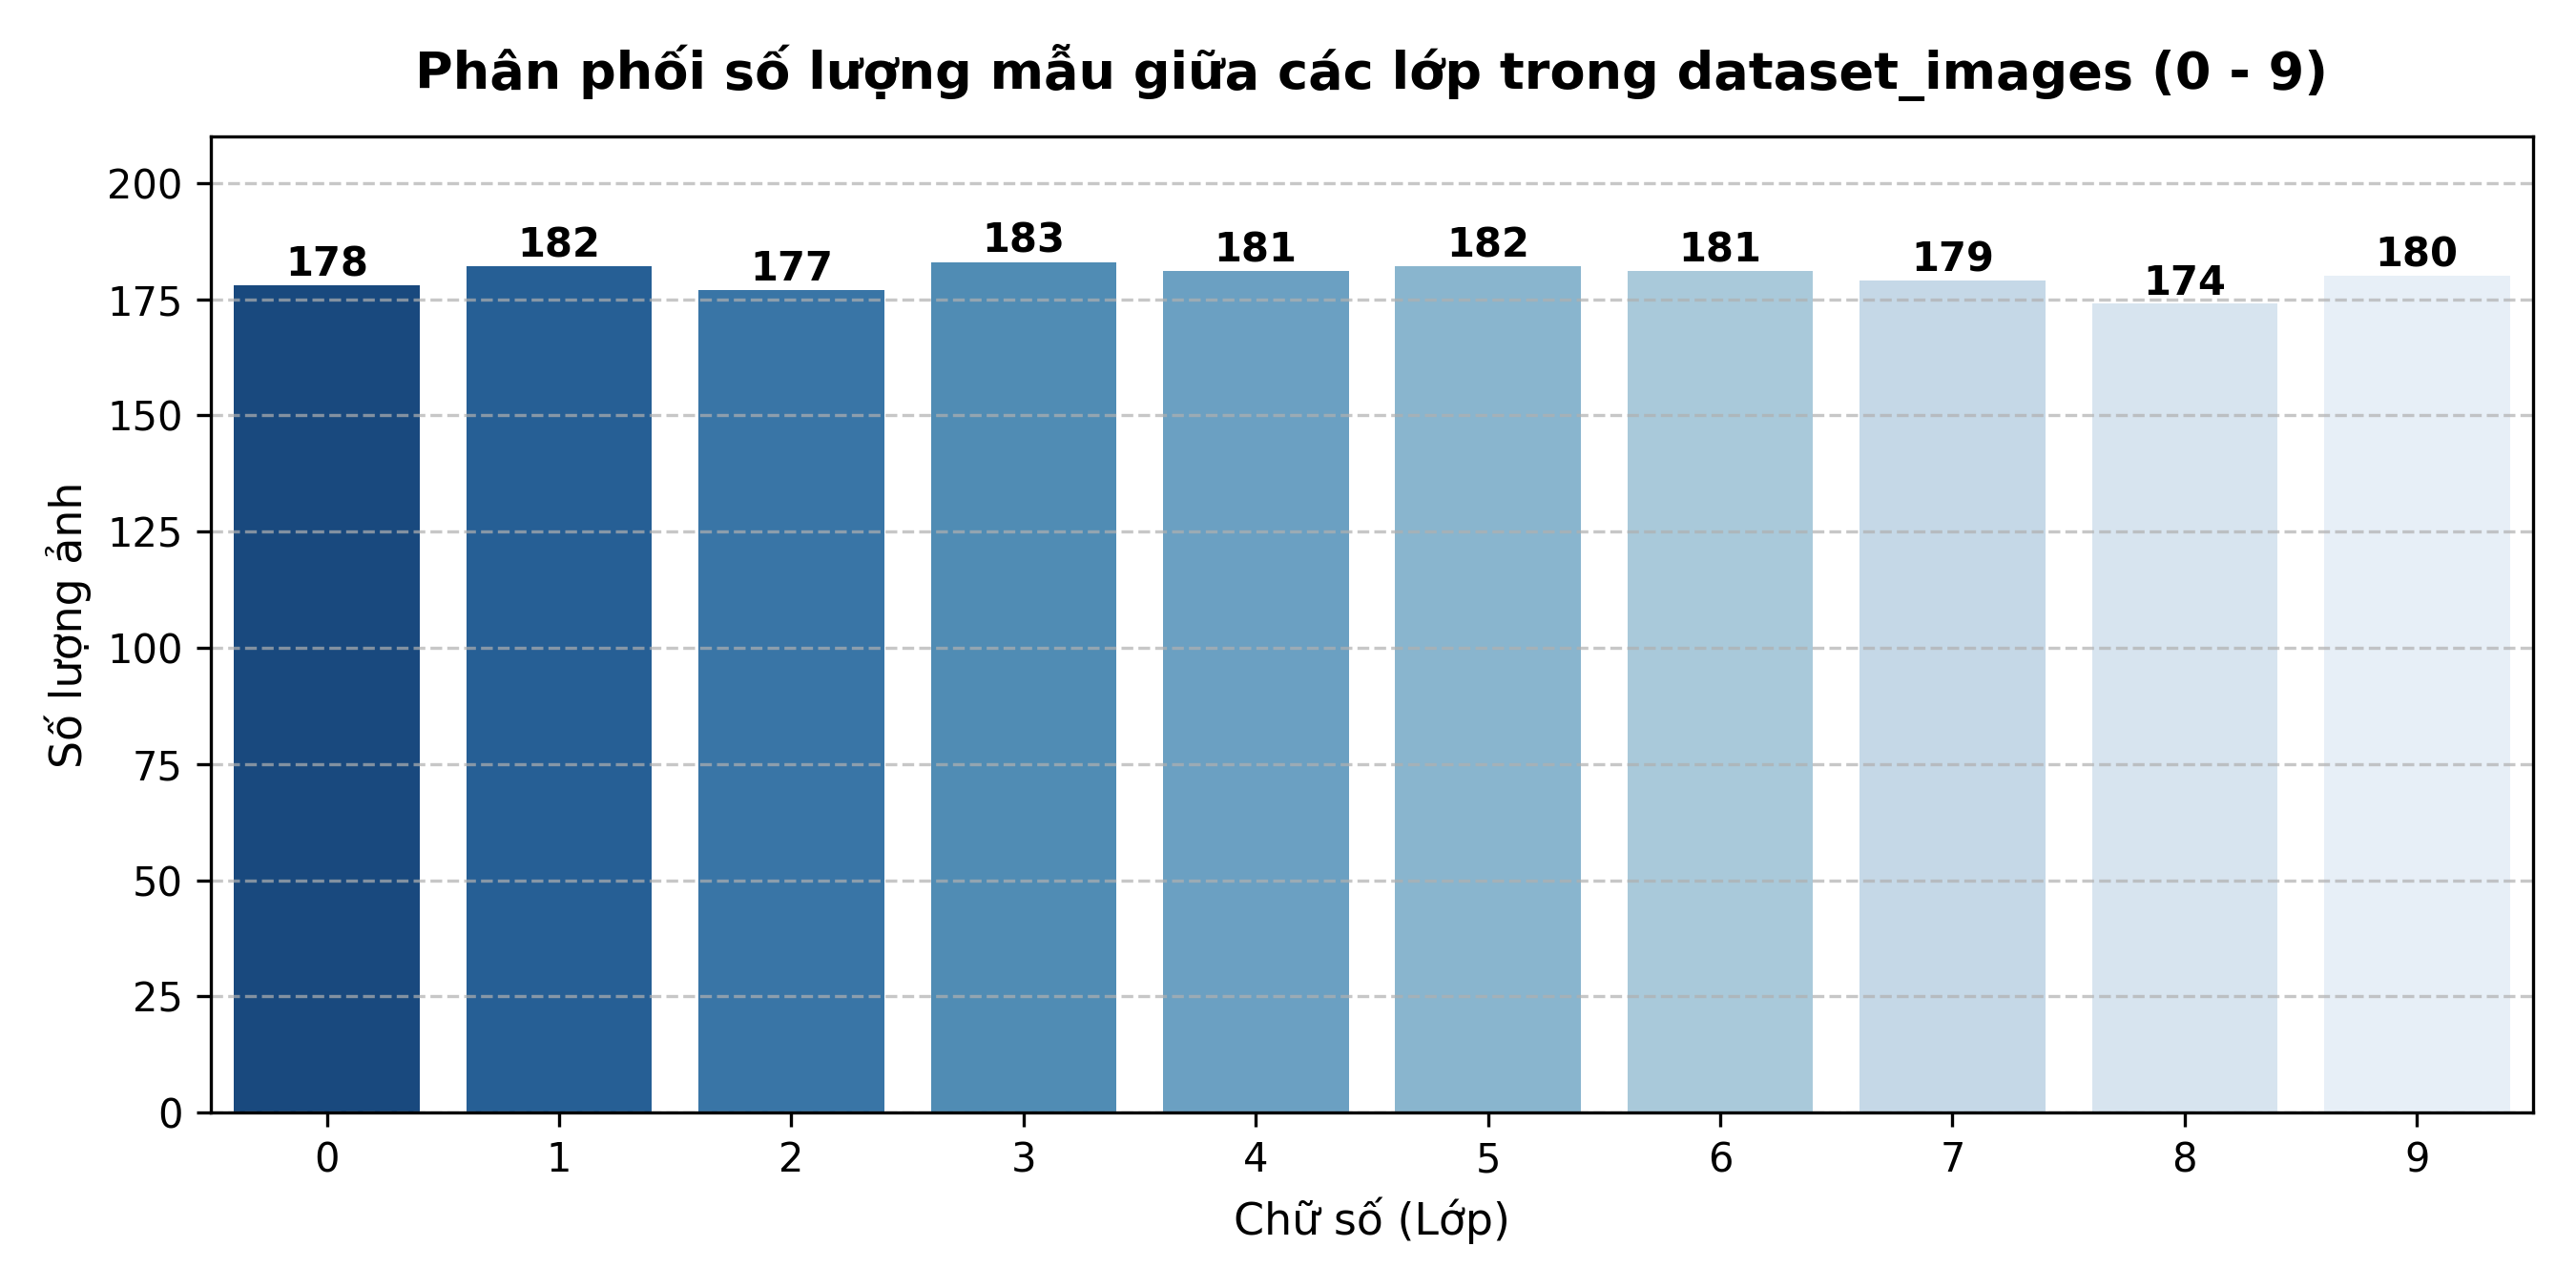
\includegraphics[width=0.75\textwidth]{figures/eda_label_distribution.png}
\caption{Phân phối số lượng ảnh giữa 10 lớp chữ số}
\label{fig:eda_label}
\end{figure}

\subsection{Trực quan hóa hình thái chữ số}

Hình~\ref{fig:eda} thể hiện một ảnh mẫu và ảnh trung bình của từng lớp. Ảnh trung bình cho thấy mỗi chữ số có
cấu trúc không gian riêng: chữ số 0 rỗng ở giữa, chữ số 1 là một dải sáng thẳng đứng và hẹp, chữ số 8 có hai
vòng chồng lên nhau. Những cặp có vùng sáng trùng nhau nhiều như 1 và 8 (khi số 8 được viết hẹp), 1 và 7, 3 và 9,
4 và 9 được dự báo là các cặp dễ nhầm lẫn. Khi đo khung bao nét chữ, nhóm nhận thấy tất cả các ảnh đều chiếm
trọn 8 hàng và phần lớn chiếm 6 trên 8 cột. Điều này chứng tỏ dữ liệu đã được căn giữa và chuẩn hóa kích thước từ
trước, và đây là điểm quan trọng khi đưa mô hình vào sử dụng với ảnh thực tế (Mục~\ref{sec:thucte}).

\begin{figure}[H]
\centering
\begin{subfigure}[t]{0.48\textwidth}
  \centering
  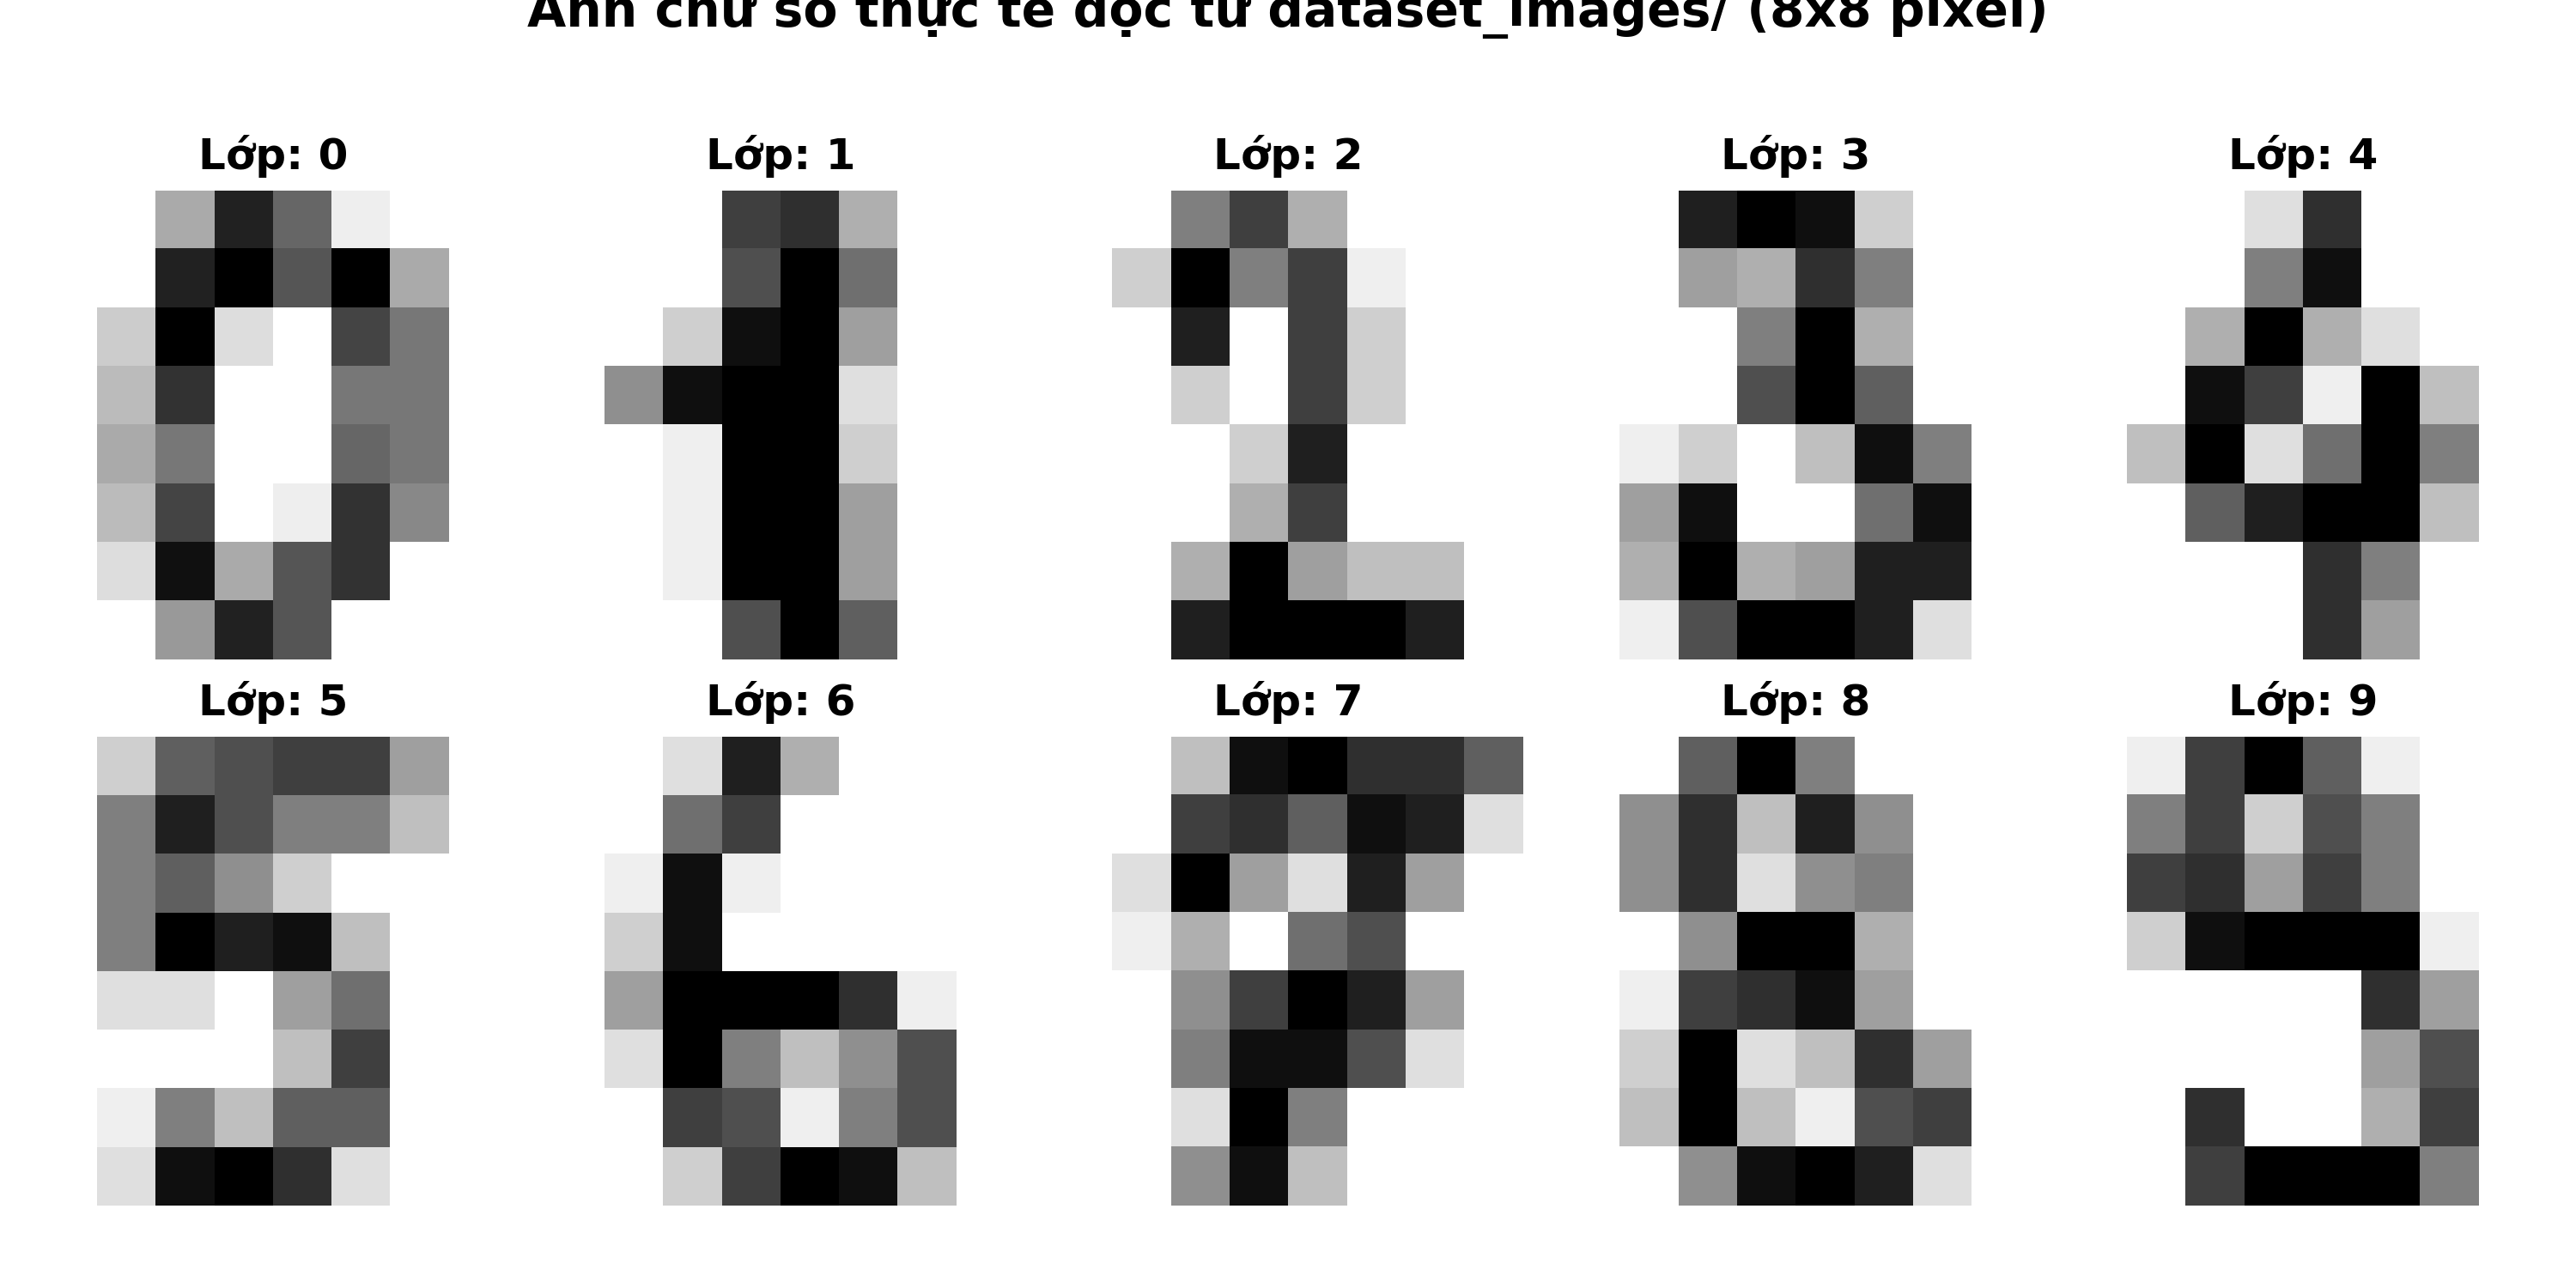
\includegraphics[width=\textwidth]{figures/eda_sample_digits.png}
  \caption{Ảnh mẫu của từng lớp}
\end{subfigure}\hfill
\begin{subfigure}[t]{0.48\textwidth}
  \centering
  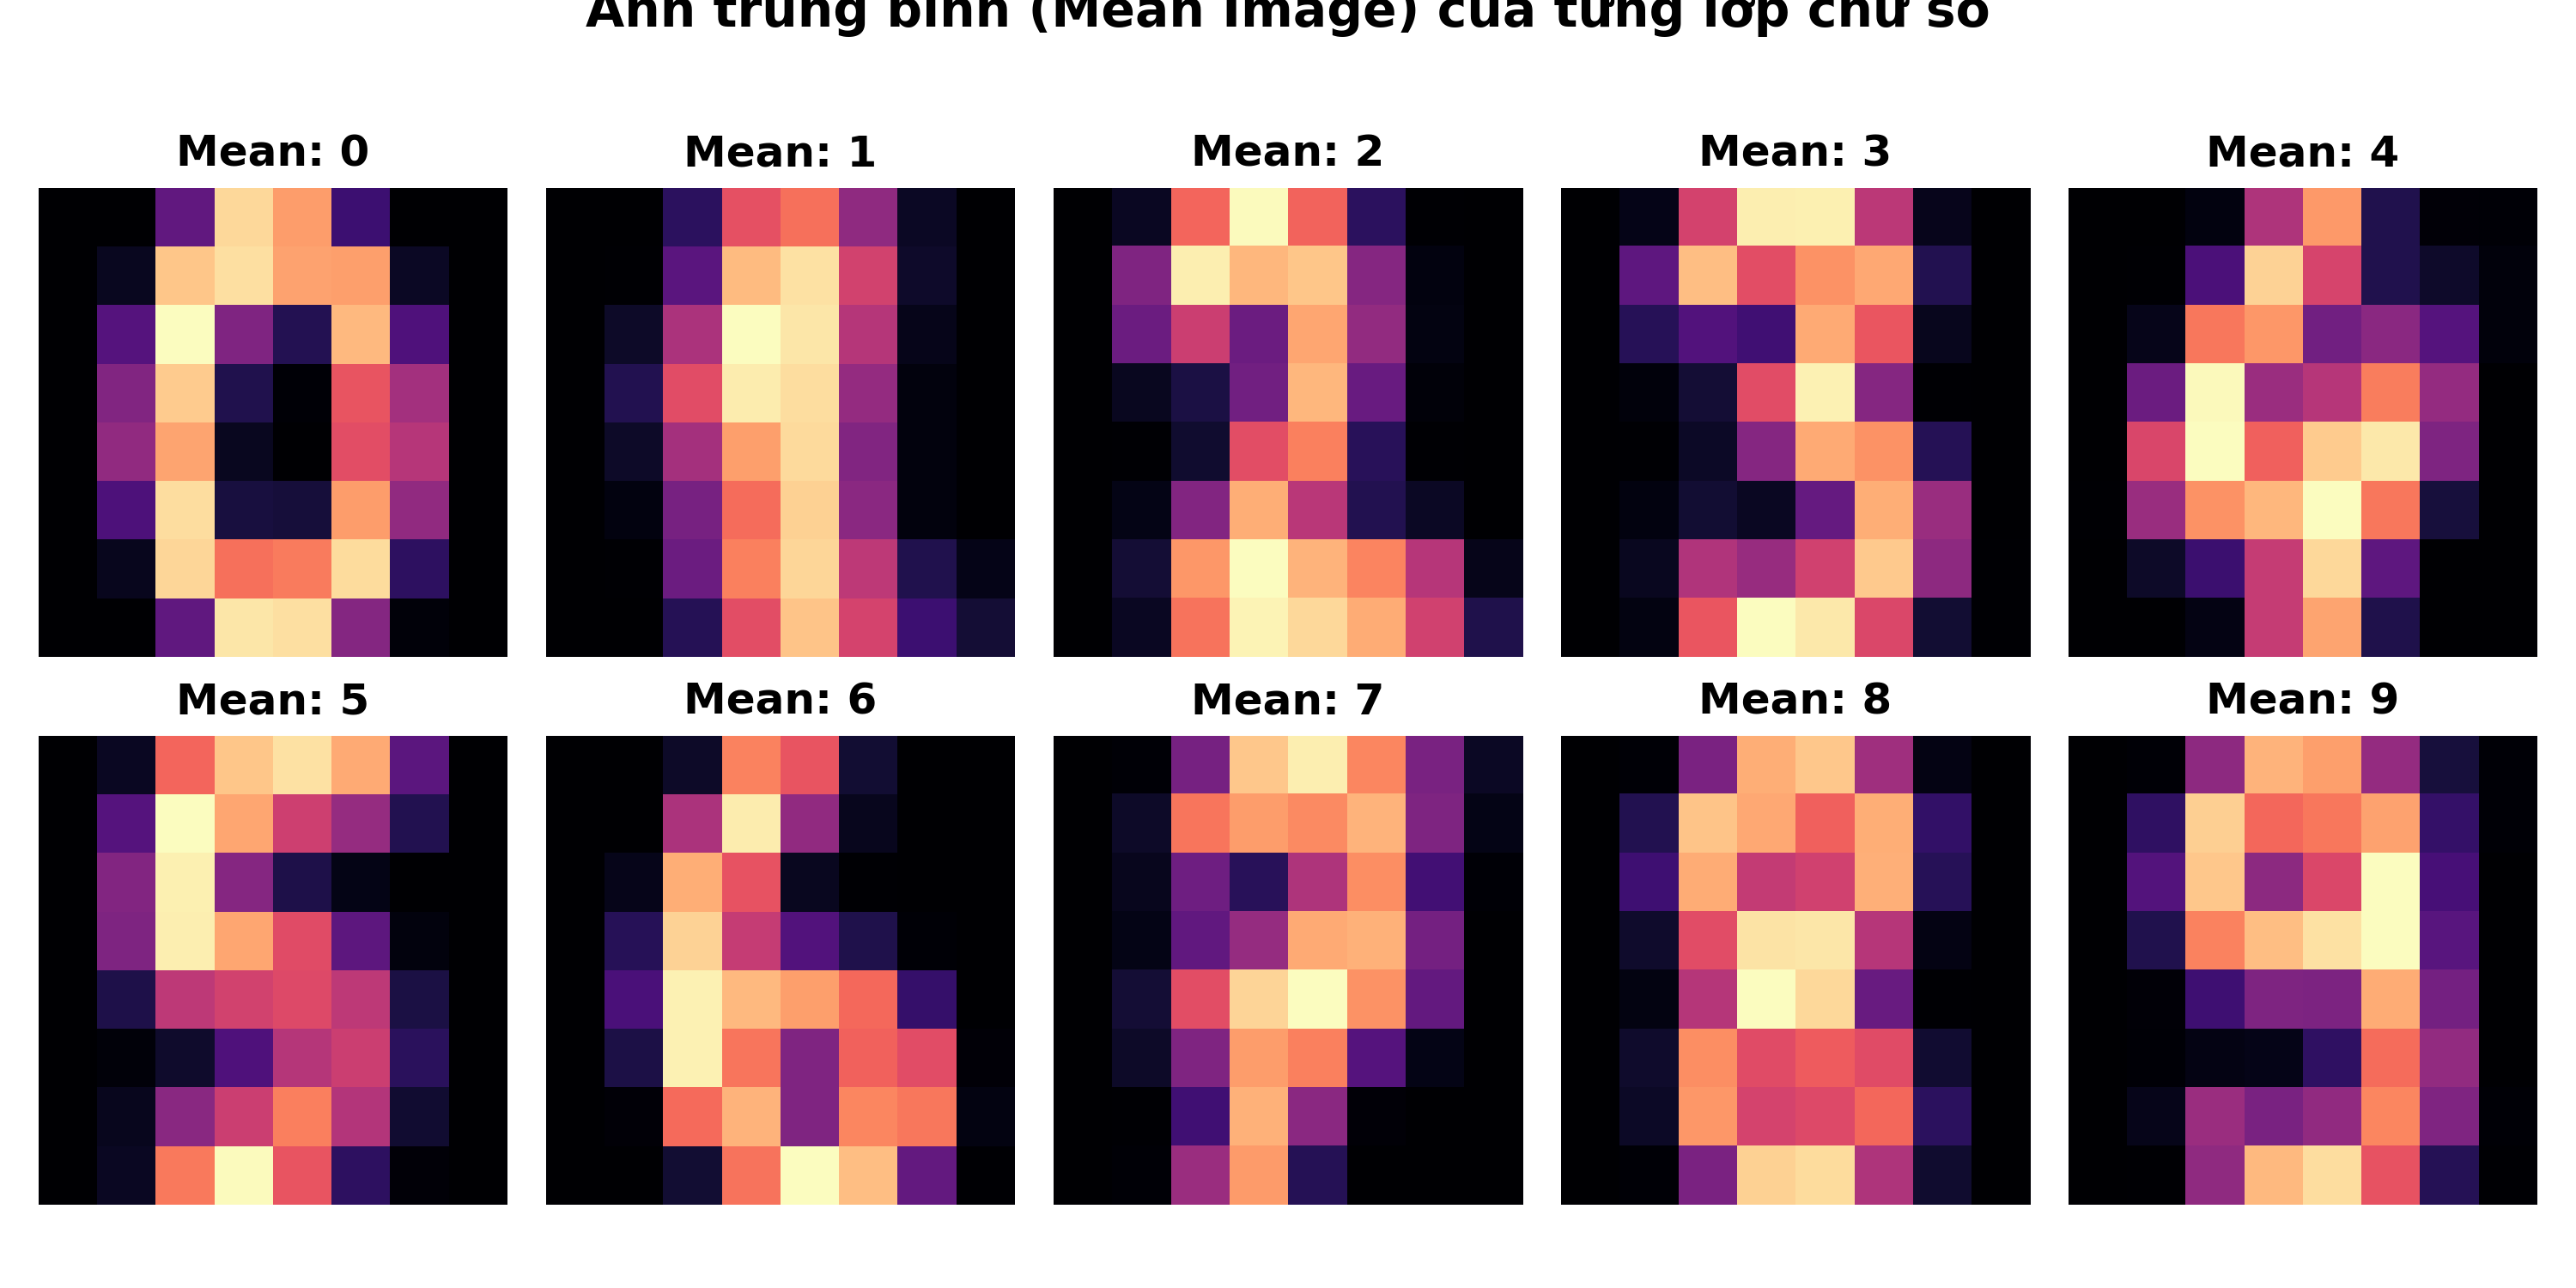
\includegraphics[width=\textwidth]{figures/eda_mean_digits.png}
  \caption{Ảnh trung bình của từng lớp}
\end{subfigure}
\caption{Trực quan hóa hình thái chữ số trong tập dữ liệu}
\label{fig:eda}
\end{figure}

\subsection{Thống kê giá trị điểm ảnh}

Để hiểu vai trò của từng vị trí trong ảnh, nhóm tính giá trị trung bình và độ lệch chuẩn của mỗi điểm ảnh trên
tập huấn luyện (Hình~\ref{fig:pixstats}). Có 48,9\% giá trị điểm ảnh trong toàn bộ dữ liệu bằng 0, tức là gần một
nửa diện tích ảnh là nền. Hai cột ngoài cùng (cột 0 và cột 7) gần như luôn tối, có 3 điểm ảnh có phương sai bằng 0
(vị trí 0, 32 và 39 khi duỗi ảnh thành vector) và 12 điểm ảnh có phương sai nhỏ hơn 0,001. Những điểm ảnh này hầu
như không mang thông tin để phân biệt các chữ số. Ngược lại, vùng trung tâm (hàng 2 đến 5, cột 2 đến 5) có độ lệch
chuẩn lớn nhất, khoảng 0,36 đến 0,41, cho thấy đây là nơi hình dạng các chữ số khác nhau nhiều nhất.

\begin{figure}[H]
\centering
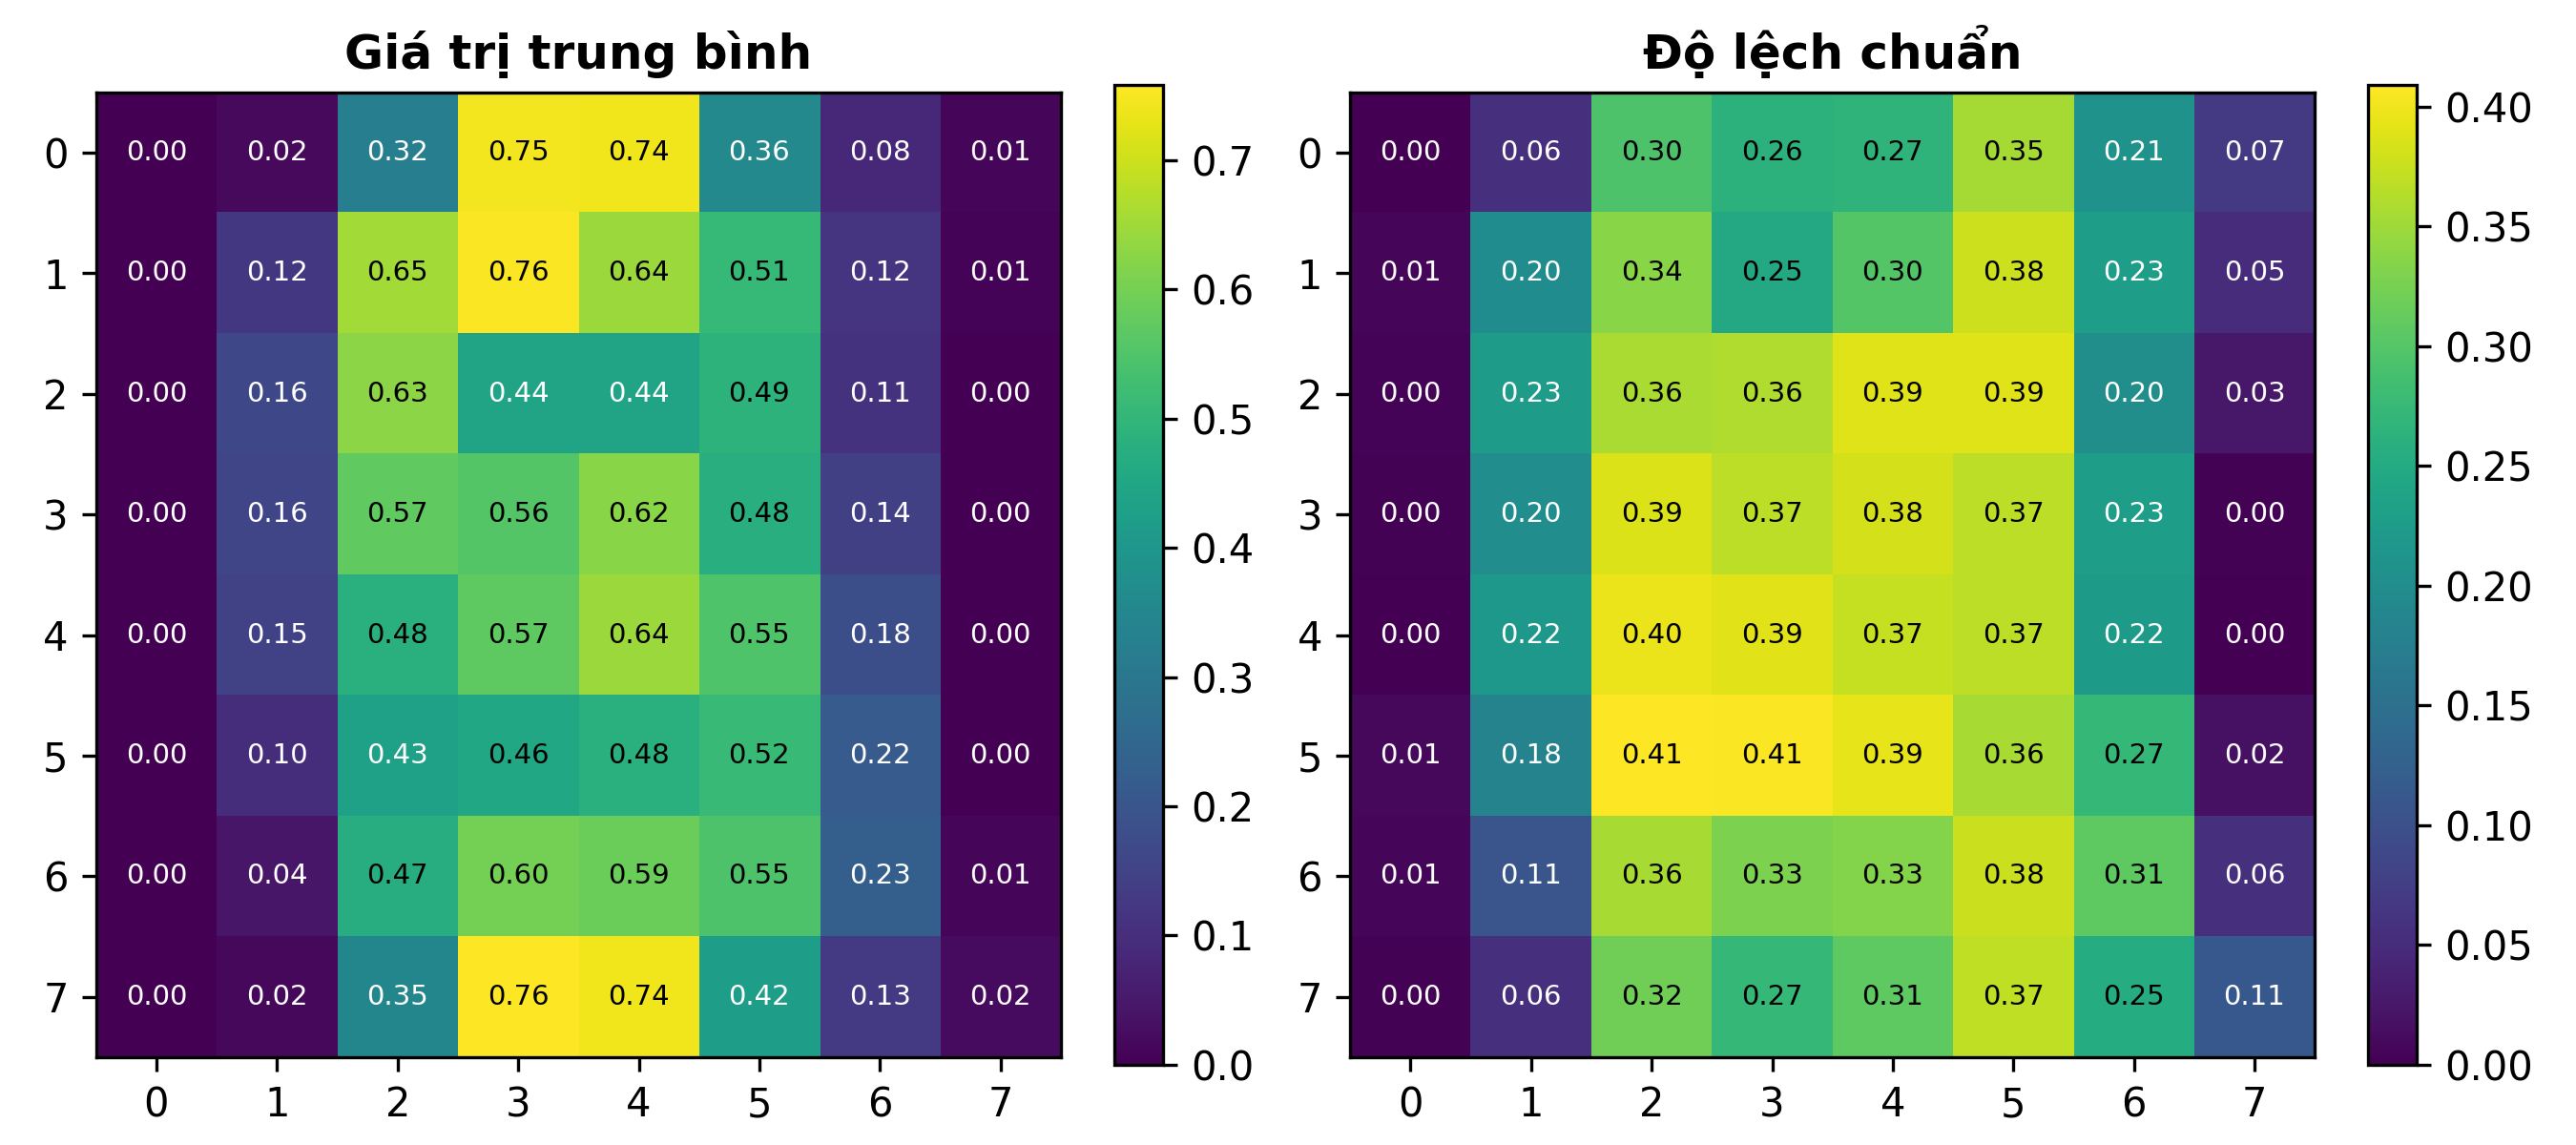
\includegraphics[width=0.9\textwidth]{figures/eda_pixel_stats.png}
\caption{Giá trị trung bình và độ lệch chuẩn của từng điểm ảnh trên tập huấn luyện}
\label{fig:pixstats}
\end{figure}

Một nhận xét đáng chú ý khác là tổng cường độ sáng của một ảnh (tương ứng với lượng ``mực'' đã dùng để viết) gần
như bằng nhau giữa các lớp, chỉ dao động từ khoảng 19,0 đến 20,7 trên thang chuẩn hóa. Như vậy, mô hình không thể
phân biệt chữ số chỉ dựa vào lượng nét, mà phải dựa vào vị trí của các nét trong ảnh. Điều này phù hợp với các
phương pháp so sánh trực tiếp theo vị trí điểm ảnh như K-NN.

\subsection{Nhận xét và giả thuyết ban đầu}

Từ các kết quả khám phá dữ liệu, nhóm đặt ra bốn giả thuyết để kiểm chứng trong các chương sau. Giả thuyết thứ
nhất: vì dữ liệu đã được căn giữa và chuẩn hóa kích thước, các phương pháp dựa trên khoảng cách giữa các vector
điểm ảnh như K-NN sẽ cho kết quả tốt. Giả thuyết thứ hai: do nhiều điểm ảnh ở rìa gần như không đổi, PCA có thể
giảm đáng kể số chiều mà vẫn giữ được độ chính xác. Giả thuyết thứ ba: ảnh quá nhỏ nên HOG với ô $2 \times 2$
khó phát huy hiệu quả. Giả thuyết thứ tư: các cặp chữ số có vùng sáng trùng nhau nhiều như 1 và 8, 1 và 7, 4 và 9
sẽ là nguồn lỗi chính.

\section{Giả định và giới hạn}

Nhóm giả định mỗi ảnh chứa đúng một chữ số đã được căn giữa, nền tối và nét sáng, giống như dữ liệu gốc. Độ
phân giải $8 \times 8$ giúp việc tính toán rất nhẹ nhưng làm mất các chi tiết nhỏ như khe hở của số 8 hay vòng
khép kín của số 9. Ngoài ra, dữ liệu chỉ đến từ 43 người viết nên sự đa dạng về nét chữ còn hạn chế, mô hình
không thể kỳ vọng đạt độ chính xác như trên tập kiểm thử khi áp dụng cho ảnh chụp ngoài thực tế nếu không có
bước chuẩn hóa ảnh tương ứng. Phạm vi của đề tài là nhận dạng từng chữ số riêng lẻ; việc nhận dạng chuỗi chữ số
chỉ được hỗ trợ ở mức ứng dụng demo thông qua bước tách chữ số đơn giản.

% ======================================================================
\chapter{THIẾT KẾ GIẢI PHÁP VÀ QUY TRÌNH HỌC MÁY}
% ======================================================================

\section{Sơ đồ quy trình}

Quy trình của nhóm tuân theo các bước tổng quát trong hướng dẫn bài tập lớn và được thể hiện trong
Hình~\ref{fig:pipeline}. Ảnh được đọc từ thư mục, khám phá và tiền xử lý, sau đó được biểu diễn theo ba cách khác
nhau. Với mỗi cách biểu diễn, hai thuật toán được tinh chỉnh bằng kiểm định chéo trên tập huấn luyện, rồi mới
được đánh giá một lần duy nhất trên tập kiểm thử. Mô hình tốt nhất được lưu lại để dùng trong ứng dụng demo.

\begin{figure}[H]
\centering
\begin{tikzpicture}[node distance=0.5cm and 0.42cm, every node/.style={font=\small},
  box/.style={draw, rounded corners=2pt, align=center, minimum height=1.25cm, text width=2.6cm},
  arr/.style={-{Stealth}, semithick}]
\node[box] (data) {Đọc ảnh PNG\\từ thư mục};
\node[box, right=of data] (eda) {Khám phá\\dữ liệu};
\node[box, right=of eda] (pre) {Ảnh xám, chia 255,\\chia Train/Test};
\node[box, right=of pre] (feat) {Raw, HOG, PCA\\(fit trên Train)};
\node[box, below=0.8cm of feat] (model) {K-NN, cây QĐ,\\CV 5 fold};
\node[box, left=of model] (eval) {Đánh giá trên\\tập Test};
\node[box, left=of eval] (err) {Phân tích lỗi};
\node[box, left=of err] (gui) {Lưu mô hình,\\ứng dụng demo};
\draw[arr] (data) -- (eda); \draw[arr] (eda) -- (pre); \draw[arr] (pre) -- (feat);
\draw[arr] (feat) -- (model); \draw[arr] (model) -- (eval); \draw[arr] (eval) -- (err); \draw[arr] (err) -- (gui);
\end{tikzpicture}
\caption{Quy trình học máy của nhóm}
\label{fig:pipeline}
\end{figure}

\section{Tiền xử lý và chia dữ liệu}

Mỗi ảnh được chuyển sang ảnh xám một kênh, sau đó giá trị điểm ảnh được chia cho 255 để đưa về đoạn $[0, 1]$:
\begin{equation}
p_{\text{norm}} = \frac{p}{255}.
\end{equation}
Khi mọi đặc trưng có cùng thang đo, khoảng cách Euclid và Manhattan của K-NN không bị chi phối bởi một vài điểm
ảnh có giá trị lớn. Đây là phép chia cho một hằng số, không học tham số từ dữ liệu, nên không gây rò rỉ thông tin.
Nhóm không dùng phép chuẩn hóa theo trung bình và độ lệch chuẩn (\texttt{StandardScaler}) vì phép biến đổi này sẽ
khuếch đại các điểm ảnh ở rìa vốn có phương sai gần bằng 0, biến nhiễu nhỏ thành khác biệt lớn khi tính khoảng cách.
Ảnh trong bộ dữ liệu đã có cùng kích thước $8 \times 8$ nên không cần bước thay đổi kích thước.

Dữ liệu được chia thành 80\% tập huấn luyện (1.437 ảnh) và 20\% tập kiểm thử (360 ảnh) bằng hàm
\texttt{train\_test\_split} với tham số \texttt{stratify=y} để giữ nguyên tỉ lệ các lớp và
\texttt{random\_state=42} để kết quả có thể tái lập. Nhờ phân tầng, mỗi lớp có từ 35 đến 37 ảnh trong tập kiểm
thử, đủ để tính các độ đo theo từng lớp.

\section{Hạn chế rò rỉ dữ liệu}

Rò rỉ dữ liệu xảy ra khi thông tin của tập kiểm thử, dù gián tiếp, được dùng trong quá trình huấn luyện hoặc lựa
chọn mô hình, khiến kết quả đánh giá cao hơn thực tế. Nhóm áp dụng ba nguyên tắc để tránh hiện tượng này. Thứ nhất,
PCA chỉ được \texttt{fit} trên tập huấn luyện, sau đó dùng \texttt{transform} cho tập kiểm thử. Thứ hai, siêu tham
số được lựa chọn bằng kiểm định chéo phân tầng 5 fold chỉ trên tập huấn luyện, với tiêu chí là độ chính xác CV
trung bình. Thứ ba, tập kiểm thử chỉ được dùng một lần để báo cáo kết quả cuối cùng và không tham gia vào bất kỳ
quyết định lựa chọn mô hình nào. Các biểu đồ tinh chỉnh tham số trong Chương 4 cũng được vẽ theo độ chính xác CV
chứ không phải theo độ chính xác kiểm thử.

\section{Biểu diễn đặc trưng}

Theo hướng dẫn của nhóm đề tài thị giác máy tính, nhóm thử nghiệm ba cách biểu diễn được tóm tắt trong
Bảng~\ref{tab:feat}. Các mục dưới đây trình bày cơ sở lý thuyết và cách tính cụ thể của từng cách biểu diễn.

\begin{table}[H]
\centering
\caption{Ba phương án biểu diễn đặc trưng}
\label{tab:feat}
\begin{tabularx}{\textwidth}{@{}p{3.2cm}cL@{}}
\toprule
\textbf{Phương án} & \textbf{Số chiều} & \textbf{Mô tả} \\
\midrule
Raw Pixels & 64 & Vector điểm ảnh sau chuẩn hóa, dùng làm mốc so sánh \\
HOG & 128 & \texttt{orientations=8}, \texttt{pixels\_per\_cell=(2,2)}, \texttt{cells\_per\_block=(1,1)} \\
PCA & 28 & Giữ 95\% phương sai của tập huấn luyện \\
\bottomrule
\end{tabularx}
\end{table}

\subsection{Điểm ảnh thô}

Ảnh $8 \times 8$ được duỗi theo từng hàng thành vector $\mathbf{x} \in [0, 1]^{64}$, trong đó phần tử thứ
$8r + c$ là giá trị điểm ảnh ở hàng $r$, cột $c$. Đây là cách biểu diễn đơn giản nhất, giữ nguyên toàn bộ thông
tin của ảnh nhưng không có tính bất biến: chỉ cần dịch chữ số sang phải một điểm ảnh, vector sẽ thay đổi ở hầu
hết các vị trí. Với bộ dữ liệu đã được căn giữa và chuẩn hóa kích thước, nhược điểm này ít ảnh hưởng.

\subsection{Lược đồ hướng gradient}

HOG \cite{hog} mô tả hình dạng của đối tượng thông qua phân bố hướng của các cạnh. Đầu tiên, gradient theo hai
phương được tính bằng các bộ lọc sai phân $[-1, 0, 1]$:
\begin{equation}
g_x(r, c) = I(r, c + 1) - I(r, c - 1), \qquad g_y(r, c) = I(r + 1, c) - I(r - 1, c),
\end{equation}
từ đó suy ra độ lớn và hướng của gradient tại mỗi điểm ảnh:
\begin{equation}
m(r, c) = \sqrt{g_x^2 + g_y^2}, \qquad \theta(r, c) = \arctan\frac{g_y}{g_x} \in [0^\circ, 180^\circ).
\end{equation}
Ảnh được chia thành các ô $2 \times 2$ điểm ảnh, tạo ra $4 \times 4 = 16$ ô. Trong mỗi ô, nhóm xây dựng lược đồ
8 khoảng hướng, mỗi khoảng rộng $22{,}5^\circ$; mỗi điểm ảnh bỏ phiếu cho khoảng hướng của nó với trọng số bằng độ
lớn gradient. Mỗi ô tạo thành một khối riêng và được chuẩn hóa độ dài, nên vector đặc trưng cuối cùng có
$16 \times 8 = 128$ chiều. Điểm cần lưu ý là mỗi lược đồ chỉ được xây dựng từ 4 điểm ảnh, trong khi HOG thường
được dùng với các ô $8 \times 8$ điểm ảnh trên ảnh lớn. Lược đồ dựa trên quá ít phiếu bầu nên dễ bị nhiễu.

\subsection{Phân tích thành phần chính}

PCA tìm một hệ trục tọa độ mới sao cho dữ liệu chiếu lên các trục đầu tiên có phương sai lớn nhất. Gọi
$\boldsymbol{\mu}$ là vector trung bình và $\mathbf{C}$ là ma trận hiệp phương sai của tập huấn luyện gồm $n$ mẫu:
\begin{equation}
\mathbf{C} = \frac{1}{n - 1} \sum_{i=1}^{n} (\mathbf{x}_i - \boldsymbol{\mu})(\mathbf{x}_i - \boldsymbol{\mu})^{\top}.
\end{equation}
Các trục chính là các vector riêng $\mathbf{v}_1, \mathbf{v}_2, \dots$ của $\mathbf{C}$, sắp xếp theo trị riêng
giảm dần $\lambda_1 \ge \lambda_2 \ge \dots$. Một mẫu được biểu diễn bằng $q$ thành phần chính đầu tiên
$z_j = \mathbf{v}_j^{\top}(\mathbf{x} - \boldsymbol{\mu})$, và tỉ lệ phương sai được giữ lại là
$\sum_{j \le q} \lambda_j / \sum_{j} \lambda_j$. Nhóm chọn $q$ nhỏ nhất sao cho tỉ lệ này đạt ít nhất 95\%.

Trên tập huấn luyện, hai thành phần chính đầu tiên đã giải thích 28,65\% phương sai; 10 thành phần giải thích
73,79\%; 20 thành phần giải thích 89,43\%; và 28 thành phần giải thích 95,03\% (Hình~\ref{fig:pca}). Sau 40 thành
phần, tỉ lệ đạt 98,83\% và đường cong gần như nằm ngang, tương ứng với các điểm ảnh ở rìa có phương sai rất nhỏ đã
được nêu ở Mục 1.4.4. PCA vì vậy giảm 56,25\% số chiều (từ 64 xuống 28) mà chỉ bỏ đi chưa tới 5\% phương sai.

\begin{figure}[H]
\centering
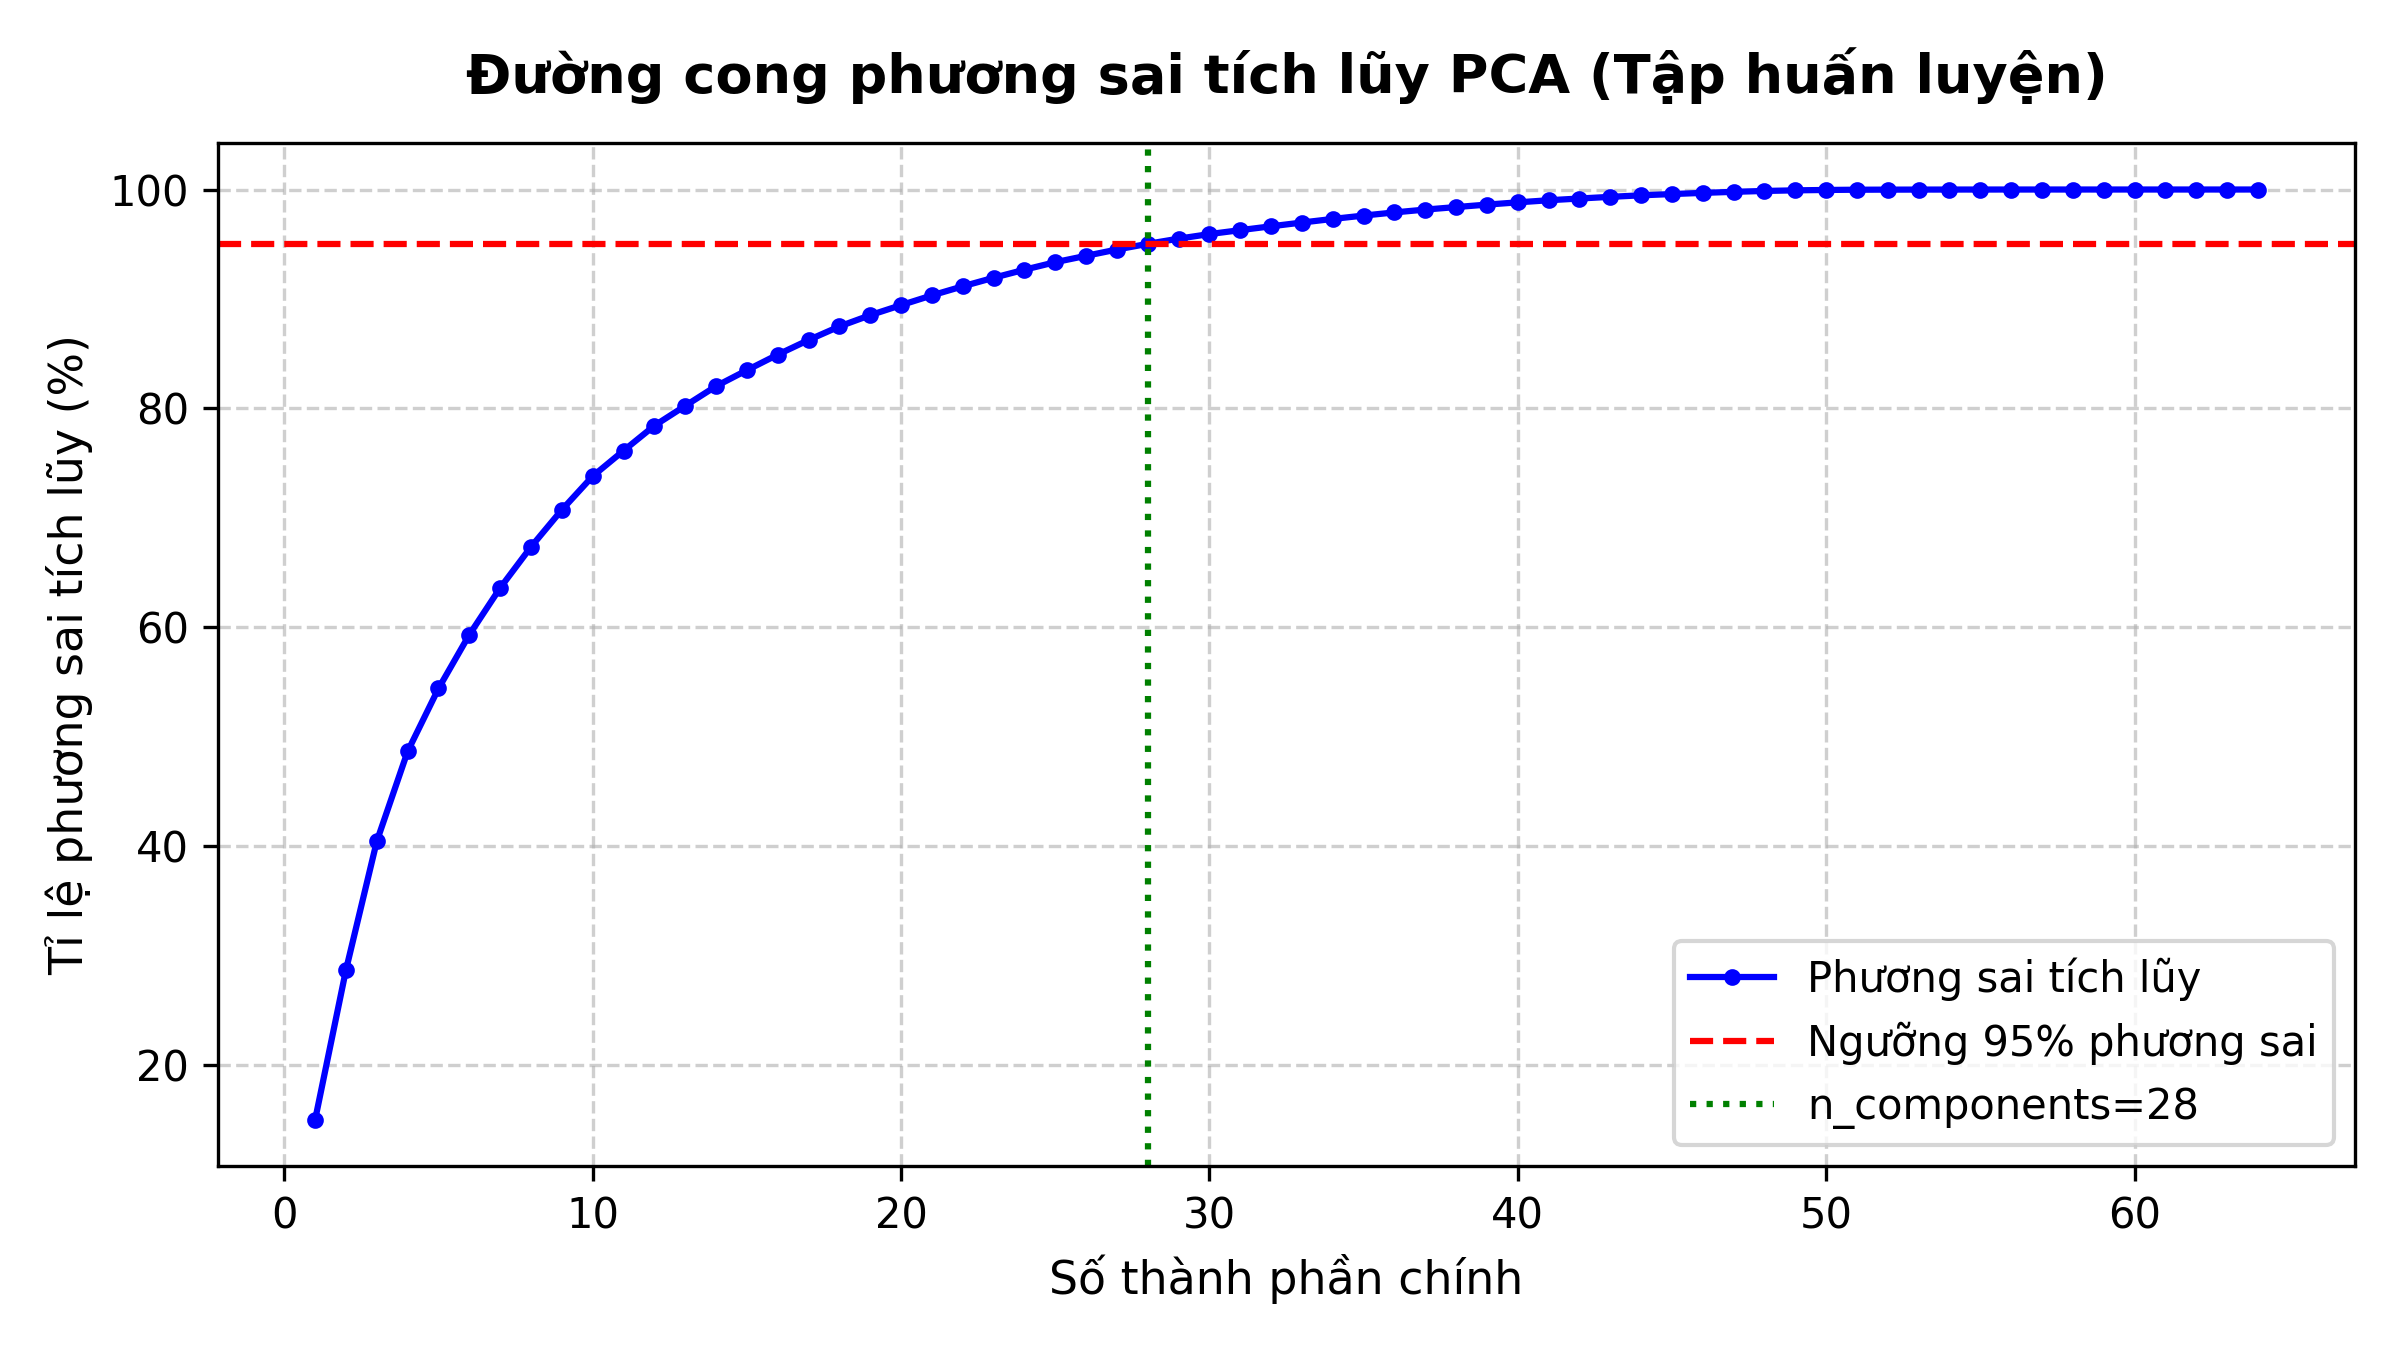
\includegraphics[width=0.7\textwidth]{figures/pca_explained_variance.png}
\caption{Phương sai tích lũy của PCA trên tập huấn luyện}
\label{fig:pca}
\end{figure}

\section{Thuật toán phân loại}

\subsection{K láng giềng gần nhất}

K-NN \cite{esl} là thuật toán học dựa trên mẫu. Ở giai đoạn huấn luyện, thuật toán chỉ lưu lại toàn bộ tập huấn
luyện. Khi cần dự đoán cho một mẫu mới $\mathbf{x}$, thuật toán tính khoảng cách từ $\mathbf{x}$ tới mọi mẫu huấn
luyện, chọn ra $k$ mẫu gần nhất và gán cho $\mathbf{x}$ nhãn xuất hiện nhiều nhất trong $k$ mẫu đó. Nhóm thử hai
loại khoảng cách:
\begin{equation}
d_{L_2}(\mathbf{x}, \mathbf{z}) = \sqrt{\sum_{j=1}^{D} (x_j - z_j)^2}, \qquad
d_{L_1}(\mathbf{x}, \mathbf{z}) = \sum_{j=1}^{D} \lvert x_j - z_j \rvert.
\end{equation}
Khoảng cách Euclid ($L_2$) phạt nặng các khác biệt lớn tại một vài điểm ảnh, còn khoảng cách Manhattan ($L_1$) cộng
dồn mọi khác biệt như nhau. Tỉ lệ phiếu bầu của từng lớp trong $k$ láng giềng được dùng làm xác suất dự đoán; với
$k = 3$, xác suất của lớp được chọn chỉ có thể là $1/3$, $2/3$ hoặc $1$, và đây chính là độ tin cậy mà ứng dụng
demo hiển thị.

Tham số $k$ điều khiển sự đánh đổi giữa độ chệch và phương sai. Với $k$ nhỏ, ranh giới quyết định bám sát từng mẫu
huấn luyện nên dễ bị ảnh hưởng bởi mẫu nhiễu; với $k$ lớn, ranh giới trơn hơn nhưng có thể bỏ qua các chi tiết phân
biệt giữa những lớp gần nhau. Chi phí dự đoán của K-NN tỉ lệ với $N \cdot D$, trong đó $N$ là số mẫu huấn luyện và
$D$ là số chiều, nên PCA giúp giảm chi phí này. Nhóm chọn K-NN vì dữ liệu đã được căn giữa và chuẩn hóa kích thước,
nên hai ảnh trông giống nhau thì vector của chúng cũng gần nhau. Các giá trị $k$ được thử là 1, 3, 5, 7, 9, 11 và
15, kết hợp với hai loại khoảng cách.

\subsection{Cây quyết định}

Cây quyết định phân chia không gian dữ liệu một cách đệ quy. Tại mỗi nút, thuật toán CART trong scikit-learn xét
mọi đặc trưng $j$ và mọi ngưỡng $t$, chia tập mẫu $S$ tại nút thành hai phần $S_L = \{x_j \le t\}$ và
$S_R = \{x_j > t\}$, rồi chọn phép chia làm giảm nhiều nhất độ bất thuần:
\begin{equation}
\Delta I = I(S) - \frac{|S_L|}{|S|} I(S_L) - \frac{|S_R|}{|S|} I(S_R),
\end{equation}
trong đó độ bất thuần $I$ được đo bằng chỉ số Gini hoặc entropy:
\begin{equation}
\text{Gini}(S) = 1 - \sum_{c} p_c^2, \qquad H(S) = -\sum_{c} p_c \log_2 p_c,
\end{equation}
với $p_c$ là tỉ lệ mẫu thuộc lớp $c$ tại nút. Với 10 lớp cân bằng, nút gốc có Gini bằng $1 - 10 \times 0{,}1^2 =
0{,}9$ và entropy bằng $\log_2 10 \approx 3{,}32$ bit; một nút chỉ chứa một lớp có độ bất thuần bằng 0. Quá trình
chia dừng lại khi nút đã thuần nhất hoặc khi cây đạt độ sâu tối đa \texttt{max\_depth}. Mức độ quan trọng của một
đặc trưng được tính bằng tổng mức giảm độ bất thuần tại các nút sử dụng đặc trưng đó.

Cây quyết định cho mô hình dạng luật, dễ diễn giải và dự đoán rất nhanh vì chỉ cần đi từ gốc xuống lá qua tối đa
\texttt{max\_depth} phép so sánh. Tuy nhiên, mỗi phép chia chỉ xét một điểm ảnh với một ngưỡng nên ranh giới quyết
định luôn song song với các trục tọa độ, và cây càng sâu càng dễ học thuộc nhiễu của tập huấn luyện. Các giá trị
được thử là \texttt{max\_depth} $\in \{3, 5, 8, 10, 15, \text{None}\}$ và \texttt{criterion} $\in$
\{gini, entropy\}, cố định \texttt{random\_state=42}.

\textbf{Phương án baseline} là K-NN với $k = 1$ và khoảng cách Euclid trên điểm ảnh thô, tức cấu hình đơn giản
nhất của K-NN: mỗi ảnh mới được gán nhãn của ảnh huấn luyện giống nó nhất.

\section{Kiểm định chéo và lựa chọn siêu tham số}

Trong kiểm định chéo phân tầng 5 fold, tập huấn luyện 1.437 ảnh được chia thành 5 phần có tỉ lệ lớp như nhau. Mỗi
cấu hình được huấn luyện 5 lần, mỗi lần trên 4 phần (khoảng 1.150 ảnh) và đánh giá trên phần còn lại (khoảng 287
ảnh). Kết quả của một cấu hình là trung bình và độ lệch chuẩn của 5 lần đánh giá. Độ lệch chuẩn cho biết mức độ ổn
định: hai cấu hình có chênh lệch trung bình nhỏ hơn độ lệch chuẩn được xem là tương đương.

Nhóm sử dụng cách tìm kiếm theo lưới: mọi tổ hợp tham số trong phạm vi đã nêu đều được thử, với tổng cộng 31 cấu
hình và 155 lần huấn luyện trong kiểm định chéo. Cấu hình có độ chính xác CV trung bình cao nhất được chọn làm mô
hình cuối cùng của mỗi thuật toán, sau đó được huấn luyện lại trên toàn bộ tập huấn luyện và đánh giá một lần trên
tập kiểm thử. Với HOG và PCA, nhóm giữ nguyên tham số tốt nhất đã chọn trên điểm ảnh thô để so sánh công bằng ảnh
hưởng của cách biểu diễn.

\section{Các độ đo đánh giá}

Với một lớp $c$, gọi $TP_c$ là số mẫu thuộc lớp $c$ được dự đoán đúng, $FP_c$ là số mẫu lớp khác bị dự đoán thành
$c$ và $FN_c$ là số mẫu lớp $c$ bị dự đoán thành lớp khác. Các độ đo được định nghĩa như sau:
\begin{equation}
\text{Precision}_c = \frac{TP_c}{TP_c + FP_c}, \qquad
\text{Recall}_c = \frac{TP_c}{TP_c + FN_c}, \qquad
F1_c = \frac{2 \cdot \text{Precision}_c \cdot \text{Recall}_c}{\text{Precision}_c + \text{Recall}_c}.
\end{equation}
Precision trả lời câu hỏi ``trong các mẫu được dự đoán là $c$, bao nhiêu mẫu đúng'', còn Recall trả lời câu hỏi
``trong các mẫu thật sự là $c$, mô hình tìm được bao nhiêu''. Giá trị macro là trung bình cộng của độ đo trên 10 lớp,
coi mọi lớp quan trọng như nhau. Accuracy là tỉ lệ mẫu được dự đoán đúng trên toàn bộ tập kiểm thử.

Ma trận nhầm lẫn là bảng $10 \times 10$, trong đó ô ở hàng $i$, cột $j$ là số mẫu thuộc lớp $i$ bị dự đoán thành lớp
$j$; các ô ngoài đường chéo chỉ ra cụ thể mô hình nhầm lớp nào với lớp nào. Đường cong ROC được xây dựng theo chiến
lược một lớp với các lớp còn lại: với mỗi lớp, xác suất dự đoán của lớp đó được dùng làm điểm số, thay đổi ngưỡng để
vẽ tỉ lệ dương tính thật theo tỉ lệ dương tính giả. Diện tích dưới đường cong (AUC) bằng 1 khi mô hình xếp hạng hoàn
hảo và bằng 0,5 khi dự đoán ngẫu nhiên.

% ======================================================================
\chapter{PHÂN TÍCH MÃ NGUỒN VÀ CHỨC NĂNG}
% ======================================================================

\section{Cấu trúc chương trình}

Mã nguồn được tổ chức thành các tệp có chức năng tách biệt như trong Bảng~\ref{tab:files}. Tệp
\nolinkurl{generate_full_project.py} chứa toàn bộ quy trình từ dữ liệu đến kết quả, đồng thời tự sinh các bảng số
liệu dùng trong báo cáo này, nhờ đó số liệu trong báo cáo luôn khớp với lần chạy thực tế.

\begin{table}[H]
\centering
\caption{Các thành phần chính của chương trình}
\label{tab:files}
\small
\begin{tabularx}{\textwidth}{@{}>{\raggedright\arraybackslash}p{7.7cm}L@{}}
\toprule
\textbf{Tệp} & \textbf{Chức năng} \\
\midrule
\texttt{main.py} & Xuất ảnh từ \texttt{load\_digits} ra thư mục \mbox{\texttt{dataset\_images/}} \\
\nolinkurl{generate_full_project.py} & Chạy toàn bộ quy trình, vẽ hình, lưu mô hình và bảng kết quả \\
\nolinkurl{handwritten_digit_recognition.ipynb} & Notebook trình bày từng bước kèm kết quả và nhận xét \\
\nolinkurl{create_notebook.py} & Sinh notebook \\
\nolinkurl{run_and_embed_notebook_outputs.py} & Chạy notebook bằng Jupyter kernel và lưu kết quả \\
\nolinkurl{gui_demo.py} & Ứng dụng giao diện đồ họa (Tkinter) \\
\nolinkurl{evaluate_gui_preprocessing.py} & Kiểm thử bước tiền xử lý ảnh của ứng dụng \\
\texttt{requirements.txt} & Danh sách thư viện cần cài đặt \\
\bottomrule
\end{tabularx}
\end{table}

Tệp \nolinkurl{generate_full_project.py} được tổ chức thành tám bước nối tiếp nhau. Bước một duyệt 10 thư mục lớp,
mở từng ảnh bằng thư viện Pillow, chuyển sang ảnh xám và chia cho 255, đồng thời kiểm tra giá trị thiếu và ảnh trùng
lặp. Bước hai chia tập huấn luyện và kiểm thử. Bước ba trích xuất đặc trưng HOG cho từng ảnh và huấn luyện PCA trên
tập huấn luyện. Bước bốn vẽ các biểu đồ khám phá dữ liệu. Bước năm chạy toàn bộ lưới tham số của K-NN và cây quyết
định thông qua một hàm đánh giá dùng chung, chọn cấu hình tốt nhất theo CV rồi thử cấu hình đó trên HOG và PCA.
Bước sáu vẽ các biểu đồ đánh giá như biểu đồ tinh chỉnh tham số, ma trận nhầm lẫn và đường cong ROC. Bước bảy thực
hiện phân tích lỗi và các phân tích bổ sung như đường cong học, mức độ quan trọng của điểm ảnh và độ tin cậy dự
đoán. Bước tám lưu mô hình tốt nhất vào \nolinkurl{best_model.pkl}, ghi bảng so sánh ra tệp CSV và sinh các bảng
\LaTeX{} dùng trong báo cáo.

Notebook \nolinkurl{handwritten_digit_recognition.ipynb} trình bày lại cùng quy trình theo từng ô lệnh, xen kẽ với
các nhận xét, để người đọc theo dõi từng bước. Notebook được chạy bằng Jupyter kernel thông qua thư viện
\texttt{nbclient}; nếu một ô lệnh bị lỗi, quá trình chạy dừng lại ngay nên kết quả lưu trong notebook luôn là kết
quả chạy thành công.

\section{Các đoạn mã quan trọng}

Đoạn mã~\ref{lst:eval} là hàm đánh giá dùng chung cho mọi thí nghiệm. Kiểm định chéo chỉ chạy trên tập huấn
luyện; sau đó mô hình được huấn luyện lại trên toàn bộ tập huấn luyện và được đo thời gian huấn luyện, thời gian
dự đoán cùng các độ đo trên tập kiểm thử. Việc dùng chung một hàm đảm bảo mọi cấu hình được đánh giá theo cùng
một cách, nên kết quả có thể so sánh trực tiếp.

\needspace{12\baselineskip}
\begin{lstlisting}[caption={Hàm đánh giá thống nhất}, label={lst:eval}]
cv = StratifiedKFold(n_splits=5, shuffle=True, random_state=42)

def evaluate_model(name, model, X_tr, X_te, y_tr, y_te, feat_name, params_str):
    cv_res = cross_validate(model, X_tr, y_tr, cv=cv, scoring=['accuracy', 'f1_macro'])
    t0 = time.perf_counter(); model.fit(X_tr, y_tr)
    train_time = (time.perf_counter() - t0) * 1000
    t0 = time.perf_counter(); preds = model.predict(X_te)
    predict_time = (time.perf_counter() - t0) * 1000
    ...
\end{lstlisting}

Đoạn mã~\ref{lst:select} thể hiện cách lựa chọn siêu tham số của K-NN theo độ chính xác CV; cây quyết định được
chọn theo cách tương tự. Đoạn mã~\ref{lst:pca} cho thấy PCA chỉ học tham số từ tập huấn luyện.

\begin{lstlisting}[caption={Chọn siêu tham số theo kiểm định chéo}, label={lst:select}]
for k in [1, 3, 5, 7, 9, 11, 15]:
    for metric in ['euclidean', 'manhattan']:
        r = evaluate_model('K-NN', KNeighborsClassifier(n_neighbors=k, metric=metric), ...)
        knn_cv[(k, metric)] = r['_cv_acc']
best_k, best_metric = max(knn_cv, key=knn_cv.get)
\end{lstlisting}

\begin{lstlisting}[caption={PCA chỉ học trên tập huấn luyện}, label={lst:pca}]
pca = PCA(n_components=0.95, random_state=42)
X_train_pca = pca.fit_transform(X_train)
X_test_pca = pca.transform(X_test)
\end{lstlisting}

Đoạn mã~\ref{lst:norm} là phần cốt lõi của bước tiền xử lý trong ứng dụng demo, đưa một chữ số bất kỳ về đúng dạng
của dữ liệu huấn luyện: chữ số được phóng cho chiếm trọn chiều cao khung $32 \times 32$, sau đó thu nhỏ về
$8 \times 8$ bằng phép lấy trung bình từng khối $4 \times 4$.

\needspace{9\baselineskip}
\begin{lstlisting}[caption={Chuẩn hóa một chữ số về dạng dữ liệu huấn luyện}, label={lst:norm}]
scale = min(32 / h, 32 / w)                      # chiem tron chieu cao khung 32x32
digit = Image.fromarray(crop).resize((round(w * scale), round(h * scale)))
frame = np.zeros((32, 32)); frame[top:top + nh, left:left + nw] = digit
arr_8x8 = Image.fromarray(frame).resize((8, 8), Image.Resampling.BOX)   # trung binh khoi 4x4
features = arr_8x8 / arr_8x8.max()
\end{lstlisting}

\section{Ứng dụng demo}
\label{sec:demo}

\subsection{Giao diện và chức năng}

Ứng dụng \nolinkurl{gui_demo.py} được xây dựng bằng thư viện Tkinter, biểu đồ được vẽ bằng Matplotlib nhúng vào cửa
sổ. Khi khởi động, ứng dụng nạp mô hình đã lưu trong \nolinkurl{best_model.pkl} và tính lại độ chính xác trên tập
kiểm thử để hiển thị ở thanh trạng thái. Giao diện gồm ba cột. Cột bên trái là vùng vẽ bằng chuột cùng thanh điều
chỉnh kích thước bút và bốn nút chức năng: nhận dạng, xóa vùng vẽ, tải ảnh từ tệp và xem mẫu ngẫu nhiên. Cột giữa
hiển thị chữ số dự đoán, độ tin cậy, biểu đồ xác suất của 10 lớp và ảnh $8 \times 8$ sau tiền xử lý, tức là ảnh mà
mô hình thực sự nhận vào. Cột bên phải liệt kê ảnh mẫu của 10 chữ số lấy từ bộ dữ liệu; khi nhấn vào một mẫu, ứng
dụng nhận dạng ngay ảnh đó. Ngoài ra, chức năng mẫu ngẫu nhiên mở một cửa sổ hiển thị 12 ảnh lấy ngẫu nhiên từ tập
kiểm thử cùng nhãn thật và nhãn dự đoán, giúp người dùng thấy được cả những trường hợp mô hình dự đoán sai.

Toàn bộ chức năng được cài đặt trong lớp \texttt{DigitRecognizerApp}. Các phương thức \texttt{\_start\_draw},
\texttt{\_draw} và \texttt{\_stop\_draw} xử lý sự kiện chuột và vẽ đồng thời lên vùng vẽ Tkinter và một ảnh Pillow
ẩn có cùng kích thước. Phương thức \texttt{\_predict\_drawn} lấy ảnh Pillow này để nhận dạng, còn
\texttt{\_load\_image} mở hộp thoại chọn tệp, xoay ảnh theo thông tin hướng chụp lưu trong ảnh của điện thoại rồi
chuyển cho \texttt{\_predict\_from\_image}. Phương thức này gọi các hàm tiền xử lý, đưa từng chữ số vào mô hình và
cập nhật kết quả lên giao diện.

\subsection{Tiền xử lý ảnh đầu vào}

Ảnh vẽ tay và ảnh chụp khác xa dữ liệu huấn luyện về kích thước, độ dày nét, màu nền và vị trí chữ số. Nếu chỉ
thu nhỏ trực tiếp ảnh về $8 \times 8$, mô hình gần như không nhận đúng được. Vì vậy, bước tiền xử lý của ứng dụng
tái hiện lại đúng cách tạo bộ dữ liệu gốc qua bốn bước sau.

a) Tách nét mực khỏi nền. Ảnh được chuyển sang ảnh xám và thu nhỏ sao cho cạnh dài không quá 800 điểm ảnh. Độ
sáng nền cục bộ được ước lượng bằng cách thu nhỏ ảnh tám lần rồi áp dụng bộ lọc lấy giá trị lớn nhất (xóa nét mực
tối) và bộ lọc trung vị (làm mượt). Lấy nền trừ đi ảnh gốc, nét mực trở thành vùng có giá trị dương lớn bất kể
ánh sáng không đều hay có bóng đổ. Ngưỡng tách nét mực được chọn tự động bằng phương pháp Otsu \cite{otsu}.

b) Loại bỏ nhiễu. Các đường ngang vừa dài hơn 60\% chiều rộng ảnh vừa mảnh được nhận diện là dòng kẻ của giấy và bị
xóa; các nét ngang của chữ số như ở số 2, 4, 5, 7 ngắn hơn hoặc dày hơn nên được giữ lại. Các thành phần liên thông
nhỏ hơn 1\% thành phần lớn nhất được coi là đốm nhiễu và bị loại bỏ.

c) Chuẩn hóa từng chữ số. Chữ số được cắt sát khung bao, phóng to sao cho chiếm trọn chiều cao khung
$32 \times 32$ và căn giữa theo chiều ngang, giống với đặc điểm của dữ liệu đã phân tích ở Mục 1.4.3. Với ảnh tải
lên, độ dày nét được chuẩn hóa bằng cách lấy bộ xương của nét (nét dày một điểm ảnh) rồi làm dày lại với bán kính
3 điểm ảnh, để nét bút bi mảnh hay nét bút dạ dày đều trở về độ dày tương tự dữ liệu gốc. Với ảnh vẽ bằng chuột,
nét vốn đã đều nên bước này được bỏ qua; hai lựa chọn này được quyết định bằng thực nghiệm ở Mục~\ref{sec:guitest}.

d) Thu nhỏ về $8 \times 8$. Ảnh $32 \times 32$ được thu nhỏ bằng cách lấy trung bình từng khối $4 \times 4$, tương
đương phép đếm điểm đen của bộ dữ liệu gốc, rồi chia cho giá trị lớn nhất để đưa về đoạn $[0, 1]$.

\subsection{Tách nhiều chữ số}

Ứng dụng cho phép viết nhiều chữ số trên cùng một dòng. Để tách các chữ số, ứng dụng tính hình chiếu của nét mực
theo cột: các cột không có nét mực liên tiếp từ 4 điểm ảnh trở lên được coi là khoảng trống giữa hai chữ số. Nếu
một đoạn có chiều rộng lớn bất thường so với chiều cao, ứng dụng hiểu rằng nhiều chữ số đang viết dính nhau. Số chữ
số được ước lượng bằng tỉ số giữa chiều rộng và 0,85 lần chiều cao, rồi mỗi vết cắt được đặt tại cột có ít nét mực
nhất trong lân cận vị trí cắt đều, tức là tại khe hẹp giữa hai chữ số. Mỗi phần sau khi tách được chuẩn hóa và nhận
dạng độc lập, kết quả được ghép theo thứ tự từ trái sang phải.

\section{Môi trường và hướng dẫn chạy lại}

{\sloppy Chương trình được phát triển và kiểm thử với Python 3.10.11 cùng các thư viện scikit-learn 1.7.2,
scikit-image 0.25.2, NumPy 2.1.3, pandas 2.3.3, Matplotlib 3.10.8, seaborn 0.13.2, Pillow 11.3.0 và joblib 1.5.3;
danh sách thư viện được khai báo trong tệp \texttt{requirements.txt}. Để chạy lại toàn bộ kết quả, người dùng thực
hiện lần lượt các lệnh trong Bảng~\ref{tab:run} tại thư mục gốc của dự án.\par}

\begin{table}[H]
\centering
\caption{Các lệnh chạy lại chương trình}
\label{tab:run}
\small
\begin{tabularx}{\textwidth}{@{}>{\raggedright\arraybackslash}p{8.3cm}L@{}}
\toprule
\textbf{Lệnh} & \textbf{Chức năng} \\
\midrule
\texttt{pip install -r requirements.txt} & Cài đặt các thư viện cần thiết \\
\texttt{python main.py} & Xuất 1.797 ảnh ra thư mục \mbox{\texttt{dataset\_images/}} \\
\texttt{python generate\_full\_project.py} & Chạy quy trình học máy, sinh hình, bảng và mô hình \\
\texttt{python create\_notebook.py} & Sinh lại notebook \\
\texttt{python run\_and\_embed\_notebook\_outputs.py} & Chạy notebook và lưu kết quả \\
\texttt{python evaluate\_gui\_preprocessing.py} & Kiểm thử tiền xử lý của ứng dụng \\
\texttt{python gui\_demo.py} & Mở ứng dụng demo \\
\bottomrule
\end{tabularx}
\end{table}

Mọi bước có tính ngẫu nhiên đều cố định \texttt{random\_state=42}, nên chạy lại sẽ cho cùng kết quả về độ chính
xác; riêng thời gian huấn luyện và dự đoán có thể dao động nhẹ tùy theo máy tính.

% ======================================================================
\chapter{THỬ NGHIỆM VÀ KẾT QUẢ}
% ======================================================================

\section{Thiết lập thí nghiệm}

Thiết lập chung của các thí nghiệm được tóm tắt trong Bảng~\ref{tab:setup}. Thời gian huấn luyện và dự đoán được
đo trên máy tính cá nhân và chỉ có ý nghĩa so sánh tương đối giữa các phương án.

\begin{table}[H]
\centering
\caption{Thiết lập thí nghiệm}
\label{tab:setup}
\begin{tabularx}{\textwidth}{@{}p{4.2cm}L@{}}
\toprule
\textbf{Hạng mục} & \textbf{Thiết lập} \\
\midrule
Chia dữ liệu & 1.437 ảnh huấn luyện, 360 ảnh kiểm thử, phân tầng, \texttt{random\_state=42} \\
Đặc trưng & Raw Pixels (64), HOG (128), PCA (28) \\
Tiêu chí chọn tham số & Độ chính xác CV trung bình 5 fold trên tập huấn luyện \\
Độ đo trên tập kiểm thử & Accuracy, Precision, Recall, F1 (macro), ma trận nhầm lẫn, ROC-AUC \\
Baseline & K-NN, $k = 1$, khoảng cách Euclid, Raw Pixels \\
\bottomrule
\end{tabularx}
\end{table}

\section{Kết quả tổng hợp}

Bảng~\ref{tab:results} trình bày kết quả của baseline và cấu hình tốt nhất (theo CV) của mỗi thuật toán trên ba
cách biểu diễn. Kết quả của toàn bộ 31 cấu hình đã chạy được trình bày trong Phụ lục~\ref{app:full}. Các giá trị
độ đo tính theo phần trăm, thời gian tính theo mili giây.

\begin{table}[H]
\centering
\caption{Kết quả của các phương án chính}
\label{tab:results}
\footnotesize
\setlength{\tabcolsep}{2.6pt}
\begin{tabular}{@{}lllcccccrr@{}}
\toprule
\textbf{Phương án} & \textbf{Đặc trưng} & \textbf{Tham số} & \textbf{CV (\%)} & \textbf{Acc} & \textbf{Prec} &
\textbf{Rec} & \textbf{F1} & \makecell[b]{\textbf{Huấn}\\\textbf{luyện}} & \makecell[b]{\textbf{Dự}\\\textbf{đoán}} \\
\midrule
\csname @@input\endcsname results_main.tex
\bottomrule
\end{tabular}
\end{table}

Baseline đạt độ chính xác CV 98,40\% và độ chính xác kiểm thử 97,78\%. Cấu hình K-NN tốt nhất theo CV là $k = 3$
với khoảng cách Euclid, đạt CV 99,03\%, độ chính xác kiểm thử 97,22\% và F1 macro 97,20\%. Cây quyết định tốt
nhất theo CV có \texttt{max\_depth=10} và tiêu chí Gini, đạt CV 85,04\% và độ chính xác kiểm thử 83,89\%. Với
K-NN, PCA cho kết quả tương đương điểm ảnh thô, còn HOG thấp hơn rõ rệt (91,94\%). Ở mọi phương án, Precision,
Recall và F1 macro đều rất gần với Accuracy, điều này phù hợp với việc dữ liệu cân bằng giữa các lớp.

\section{Tinh chỉnh siêu tham số}

\begin{figure}[H]
\centering
\begin{subfigure}[t]{0.49\textwidth}
  \centering
  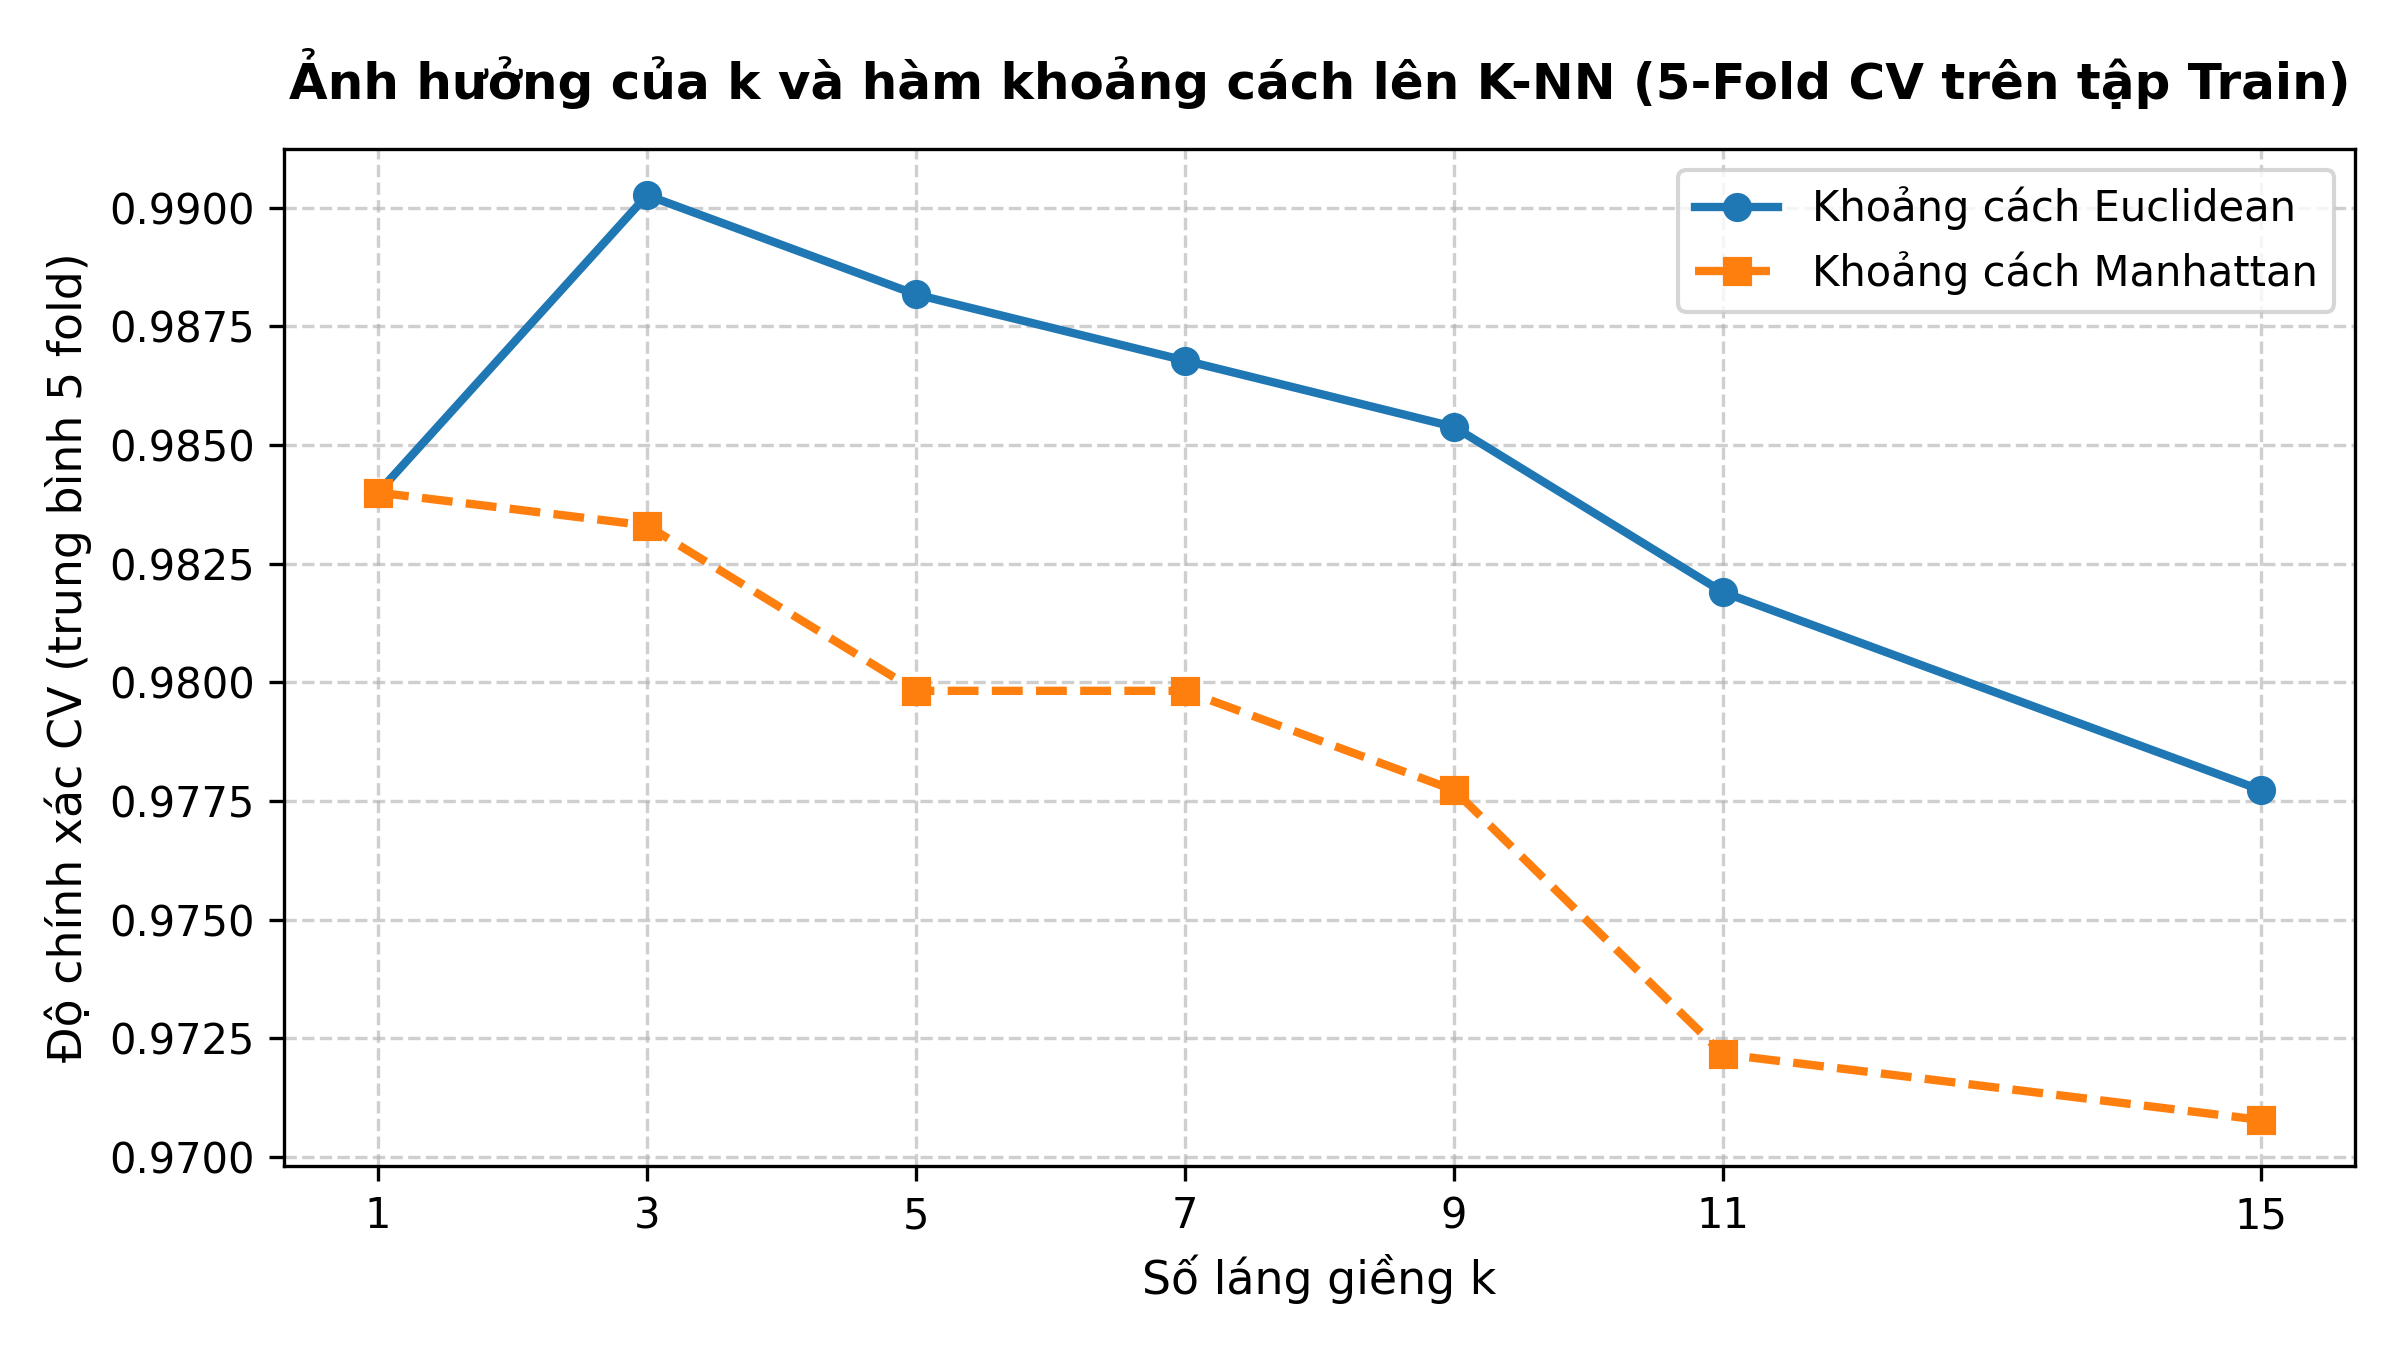
\includegraphics[width=\textwidth]{figures/knn_k_tuning.png}
  \caption{K-NN theo $k$ và khoảng cách}
\end{subfigure}\hfill
\begin{subfigure}[t]{0.49\textwidth}
  \centering
  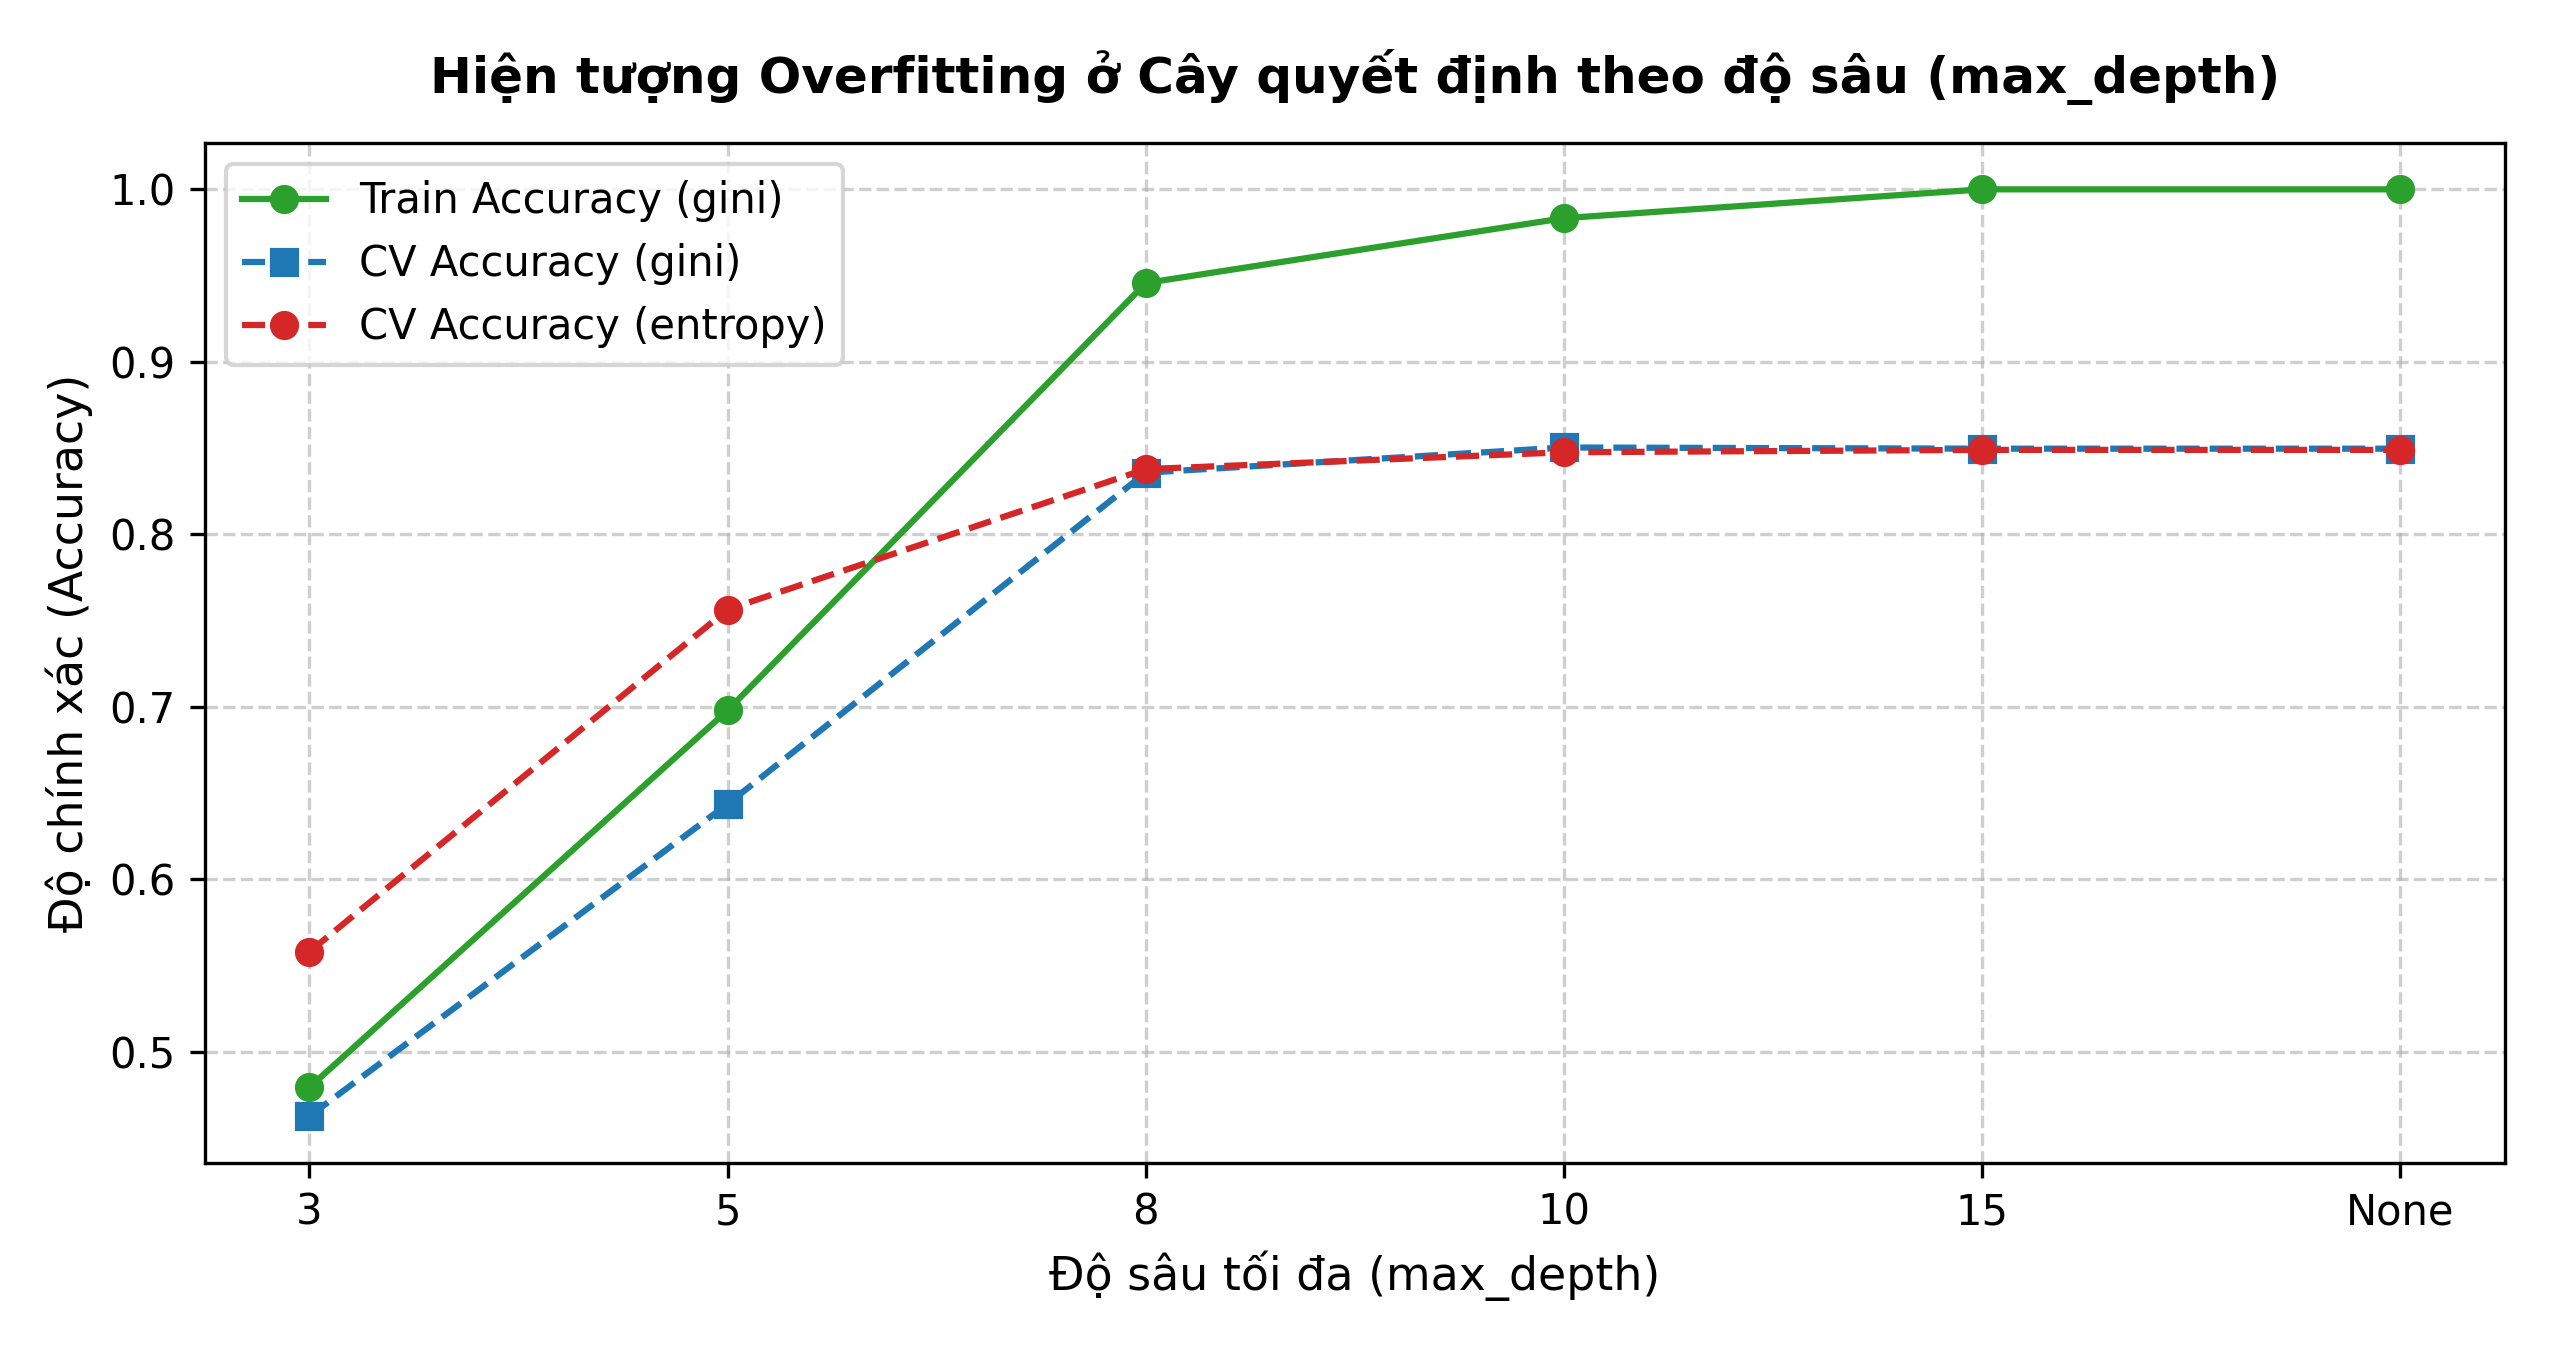
\includegraphics[width=\textwidth]{figures/dt_overfitting_curve.png}
  \caption{Cây quyết định theo độ sâu}
\end{subfigure}
\caption{Ảnh hưởng của siêu tham số đến độ chính xác kiểm định chéo}
\label{fig:tuning}
\end{figure}

Hình~\ref{fig:tuning}a cho thấy độ chính xác CV của K-NN cao nhất tại $k = 3$ và giảm dần khi $k$ tăng, do khi
có nhiều láng giềng hơn, những mẫu ở xa và thuộc lớp khác cũng tham gia bỏ phiếu. Với khoảng cách Euclid, độ chính
xác CV lần lượt là 98,40\%, 99,03\%, 98,82\%, 98,68\%, 98,54\%, 98,19\% và 97,77\% khi $k$ bằng 1, 3, 5, 7, 9, 11
và 15. Khoảng cách Manhattan cho kết quả bằng Euclid tại $k = 1$ (98,40\%) nhưng thấp hơn ở mọi giá trị $k$ còn lại,
giảm xuống 97,08\% tại $k = 15$. Lý do là khoảng cách Euclid nhấn mạnh các khác biệt lớn tại những điểm ảnh then
chốt, trong khi Manhattan cộng dồn cả các khác biệt nhỏ do nét chữ dày mỏng khác nhau. Toàn bộ các cấu hình K-NN
đều có độ lệch chuẩn CV dưới 0,9\%, cho thấy mô hình ổn định giữa các fold.

Hình~\ref{fig:tuning}b cho thấy với cây quyết định, độ chính xác trên tập huấn luyện tăng lên 100\% khi độ sâu từ
15 trở lên, trong khi độ chính xác CV dừng ở khoảng 85\% kể từ độ sâu 8. Khoảng cách lớn giữa hai đường là dấu hiệu
rõ ràng của hiện tượng quá khớp. Với cây nông, entropy tốt hơn Gini rõ rệt: ở độ sâu 3, CV của entropy là 55,81\%
so với 46,28\% của Gini; ở độ sâu 5 là 75,64\% so với 64,37\%. Nguyên nhân là entropy đánh giá cao các phép chia
tách được nhiều lớp cùng lúc, điều quan trọng khi cây chỉ có ít tầng. Khi cây đủ sâu (từ 8 trở lên), hai tiêu chí
cho kết quả gần như nhau, chênh lệch dưới 0,3\%. Độ lệch chuẩn CV của cây quyết định (0,7\% đến 2,2\%) nhìn chung lớn hơn
nhiều so với K-NN, phản ánh tính kém ổn định của mô hình cây trước những thay đổi nhỏ của dữ liệu.

\section{Ma trận nhầm lẫn và độ đo theo từng lớp}

\begin{figure}[H]
\centering
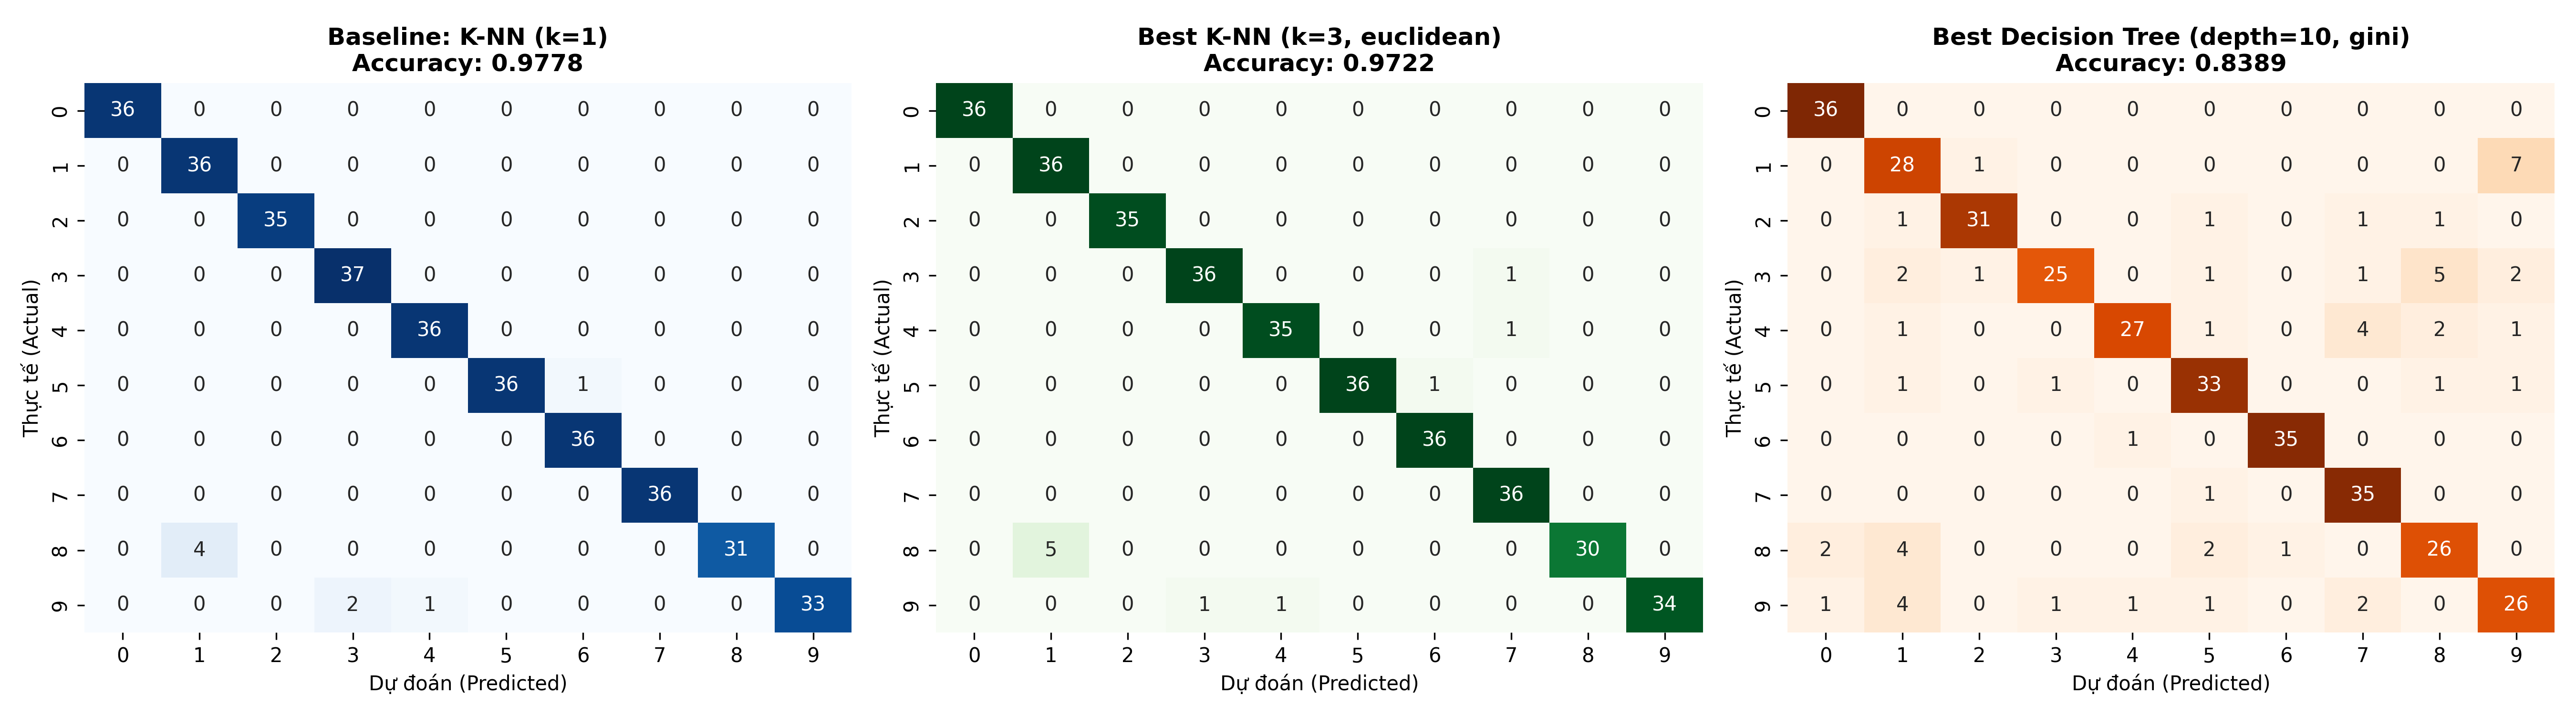
\includegraphics[width=\textwidth]{figures/confusion_matrix_comparison.png}
\caption{Ma trận nhầm lẫn trên tập kiểm thử của baseline, K-NN tốt nhất và cây quyết định tốt nhất}
\label{fig:cm}
\end{figure}

Hình~\ref{fig:cm} và Bảng~\ref{tab:perclass} cho thấy K-NN nhận dạng hoàn toàn chính xác các lớp 0 và 2. Lớp 1 có
Precision thấp nhất (87,80\%) và lớp 8 có Recall thấp nhất (85,71\%), xuất phát từ việc nhiều mẫu số 8 bị dự đoán
thành số 1. Cây quyết định có lỗi phân tán ở hầu hết các lớp, kém nhất là lớp 3 với Recall 67,57\% và lớp 9 với F1
71,23\%. Chỉ có lớp 0 và lớp 6 đạt F1 trên 95\% với cây quyết định, đây là hai chữ số có hình dạng đặc trưng nhất:
số 0 rỗng ở giữa và số 6 có vòng khép kín ở nửa dưới.

\begin{table}[H]
\centering
\caption{Precision, Recall và F1 (\%) theo từng lớp trên tập kiểm thử}
\label{tab:perclass}
\begin{tabular}{@{}cc|ccc|ccc@{}}
\toprule
\multirow{2}{*}{\textbf{Lớp}} & \multirow{2}{*}{\textbf{Số mẫu}} & \multicolumn{3}{c|}{\textbf{K-NN ($k=3$)}} &
\multicolumn{3}{c}{\textbf{Cây quyết định}} \\
 & & Prec & Rec & F1 & Prec & Rec & F1 \\
\midrule
\csname @@input\endcsname per_class_table.tex
\bottomrule
\end{tabular}
\end{table}

Đường cong ROC theo chiến lược một lớp với các lớp còn lại của K-NN tốt nhất được thể hiện trong
Hình~\ref{fig:roc}. Giá trị AUC trung bình là 0,9952; thấp nhất là lớp 8 (0,9712) và lớp 9 (0,9860), phù hợp với
phân tích ở trên. Vì K-NN với $k = 3$ chỉ cho bốn mức xác suất (0, 1/3, 2/3 và 1), đường cong ROC có dạng bậc
thang với rất ít điểm gãy.

\begin{figure}[H]
\centering
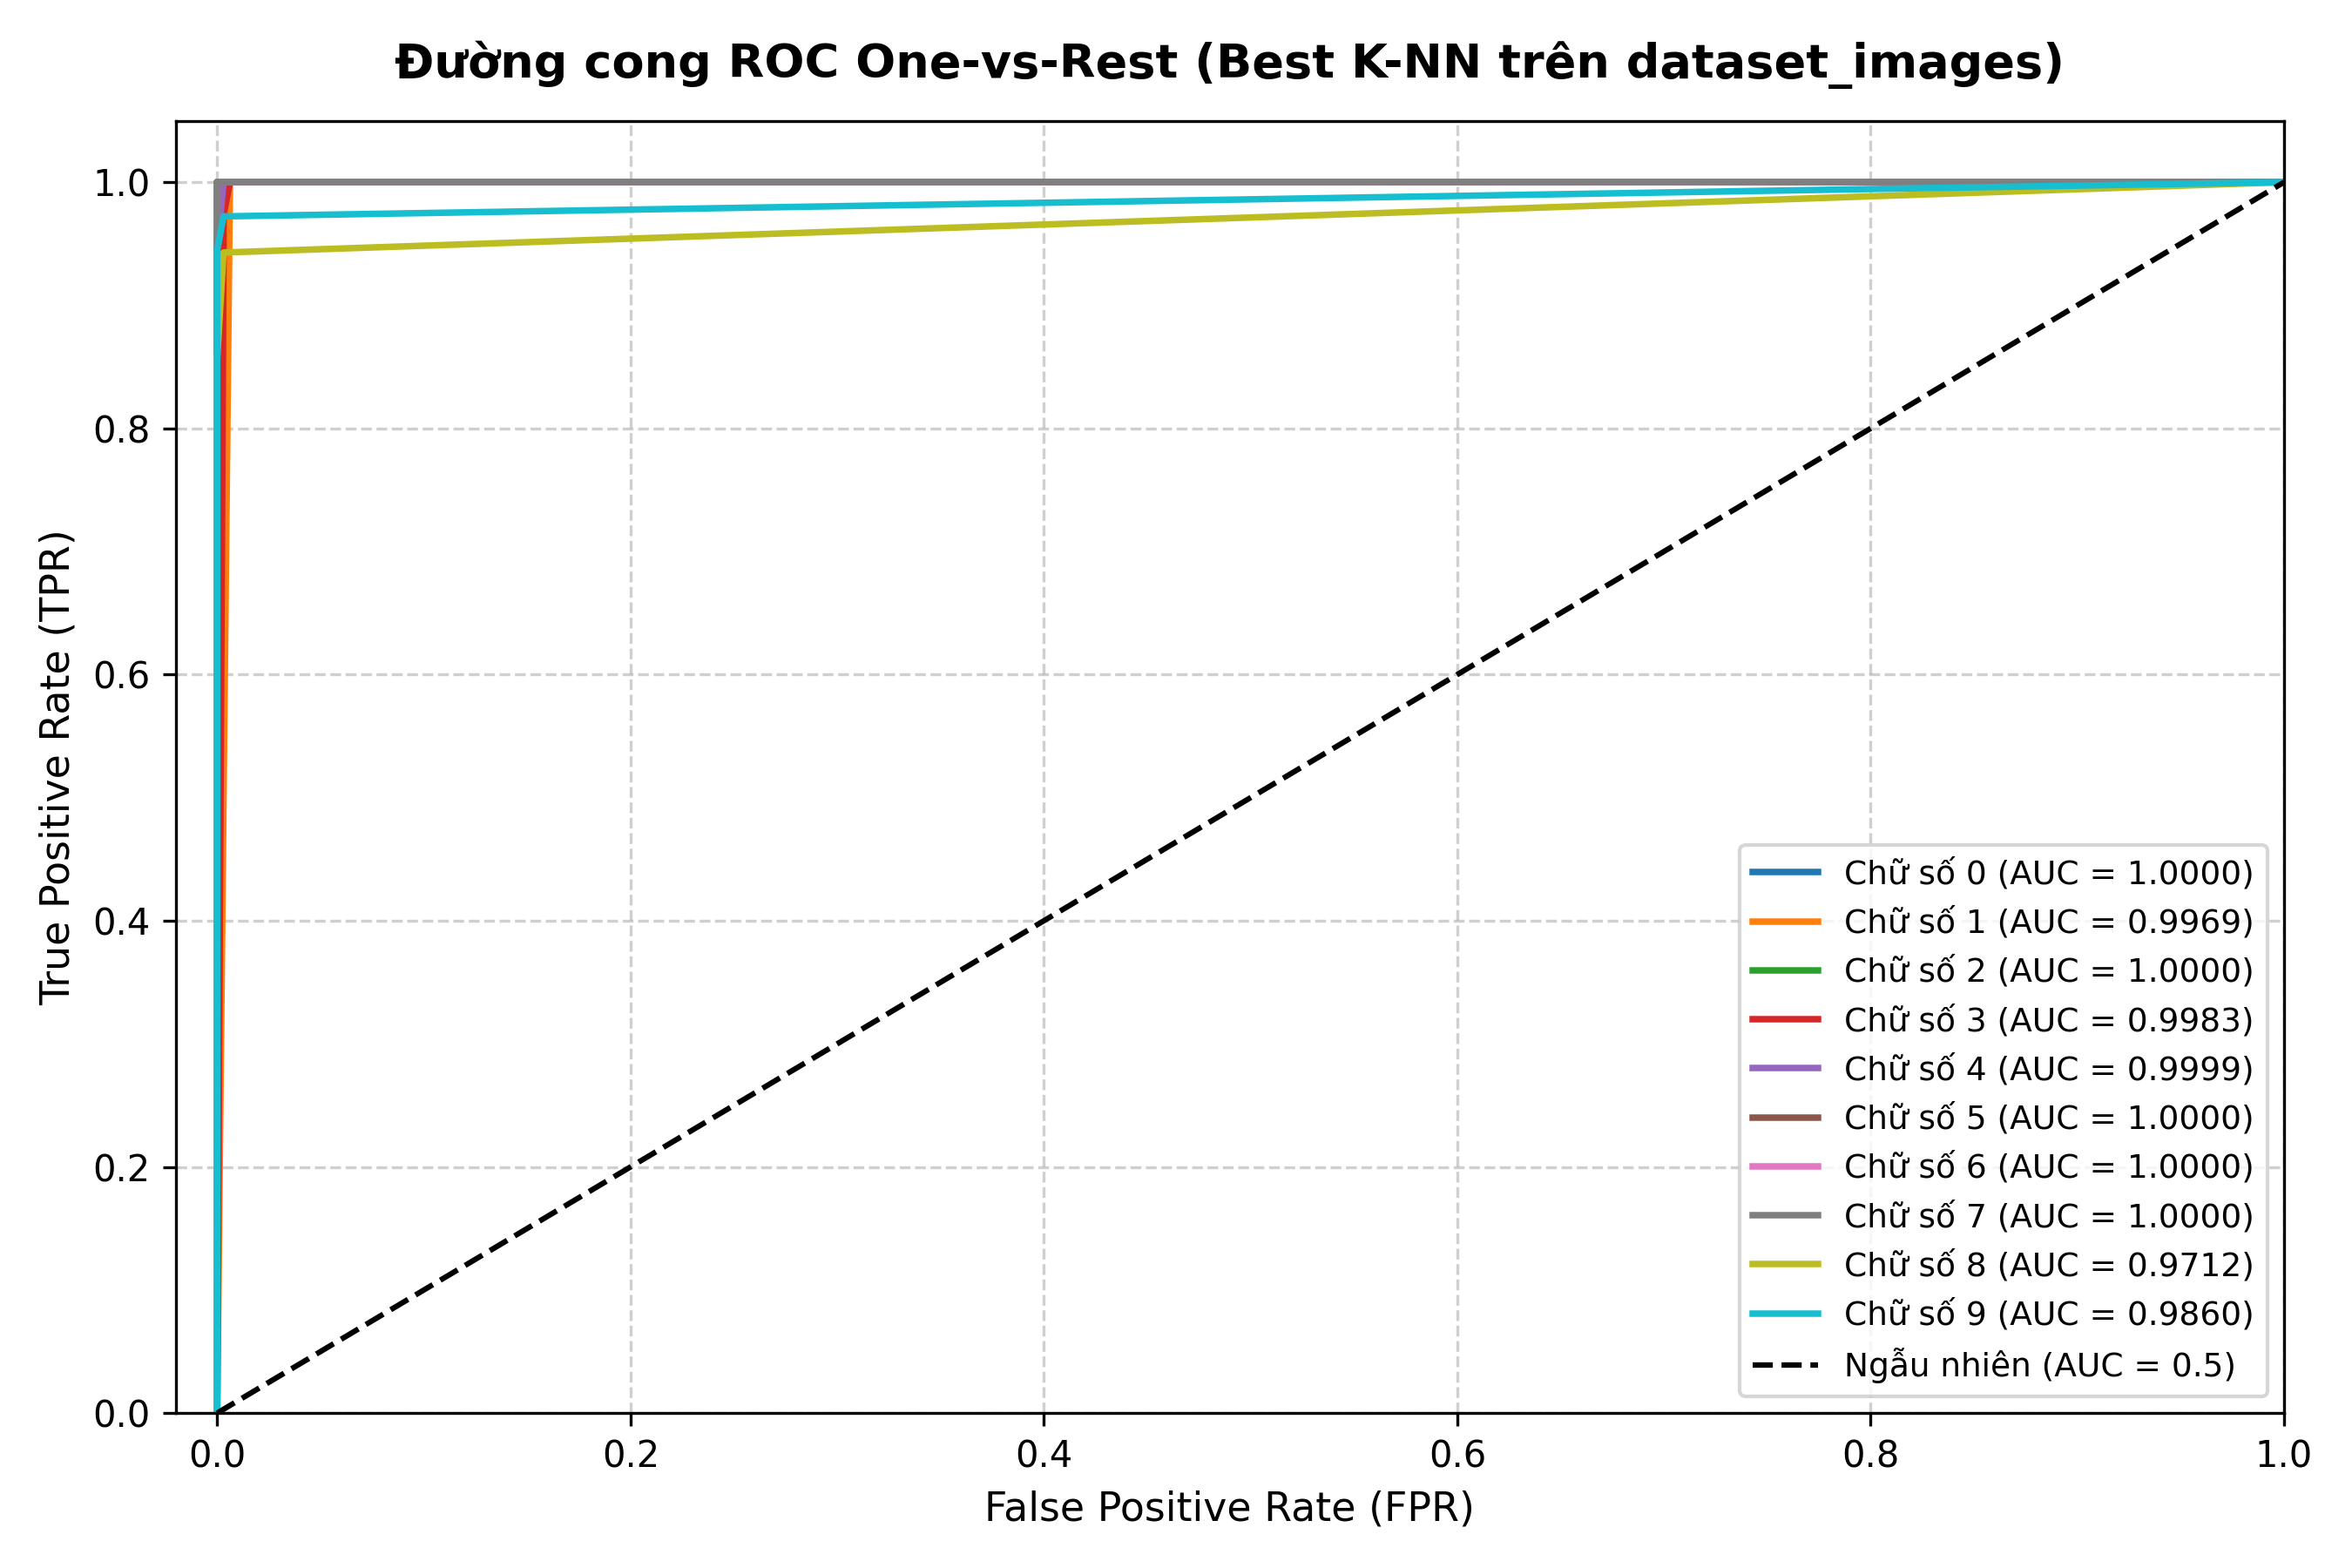
\includegraphics[width=0.68\textwidth]{figures/roc_curves_best_knn.png}
\caption{Đường cong ROC của K-NN tốt nhất}
\label{fig:roc}
\end{figure}

\section{Đường cong học}

Để trả lời câu hỏi việc có thêm dữ liệu có cải thiện mô hình hay không, nhóm vẽ đường cong học: mỗi mô hình được
huấn luyện trên 10\%, 20\%, 40\%, 60\%, 80\% và 100\% dữ liệu của từng fold huấn luyện, rồi đánh giá bằng kiểm định
chéo 5 fold. Toàn bộ thí nghiệm chỉ dùng tập huấn luyện. Kết quả được trình bày trong Hình~\ref{fig:lc} và
Bảng~\ref{tab:lc}.

\begin{figure}[H]
\centering
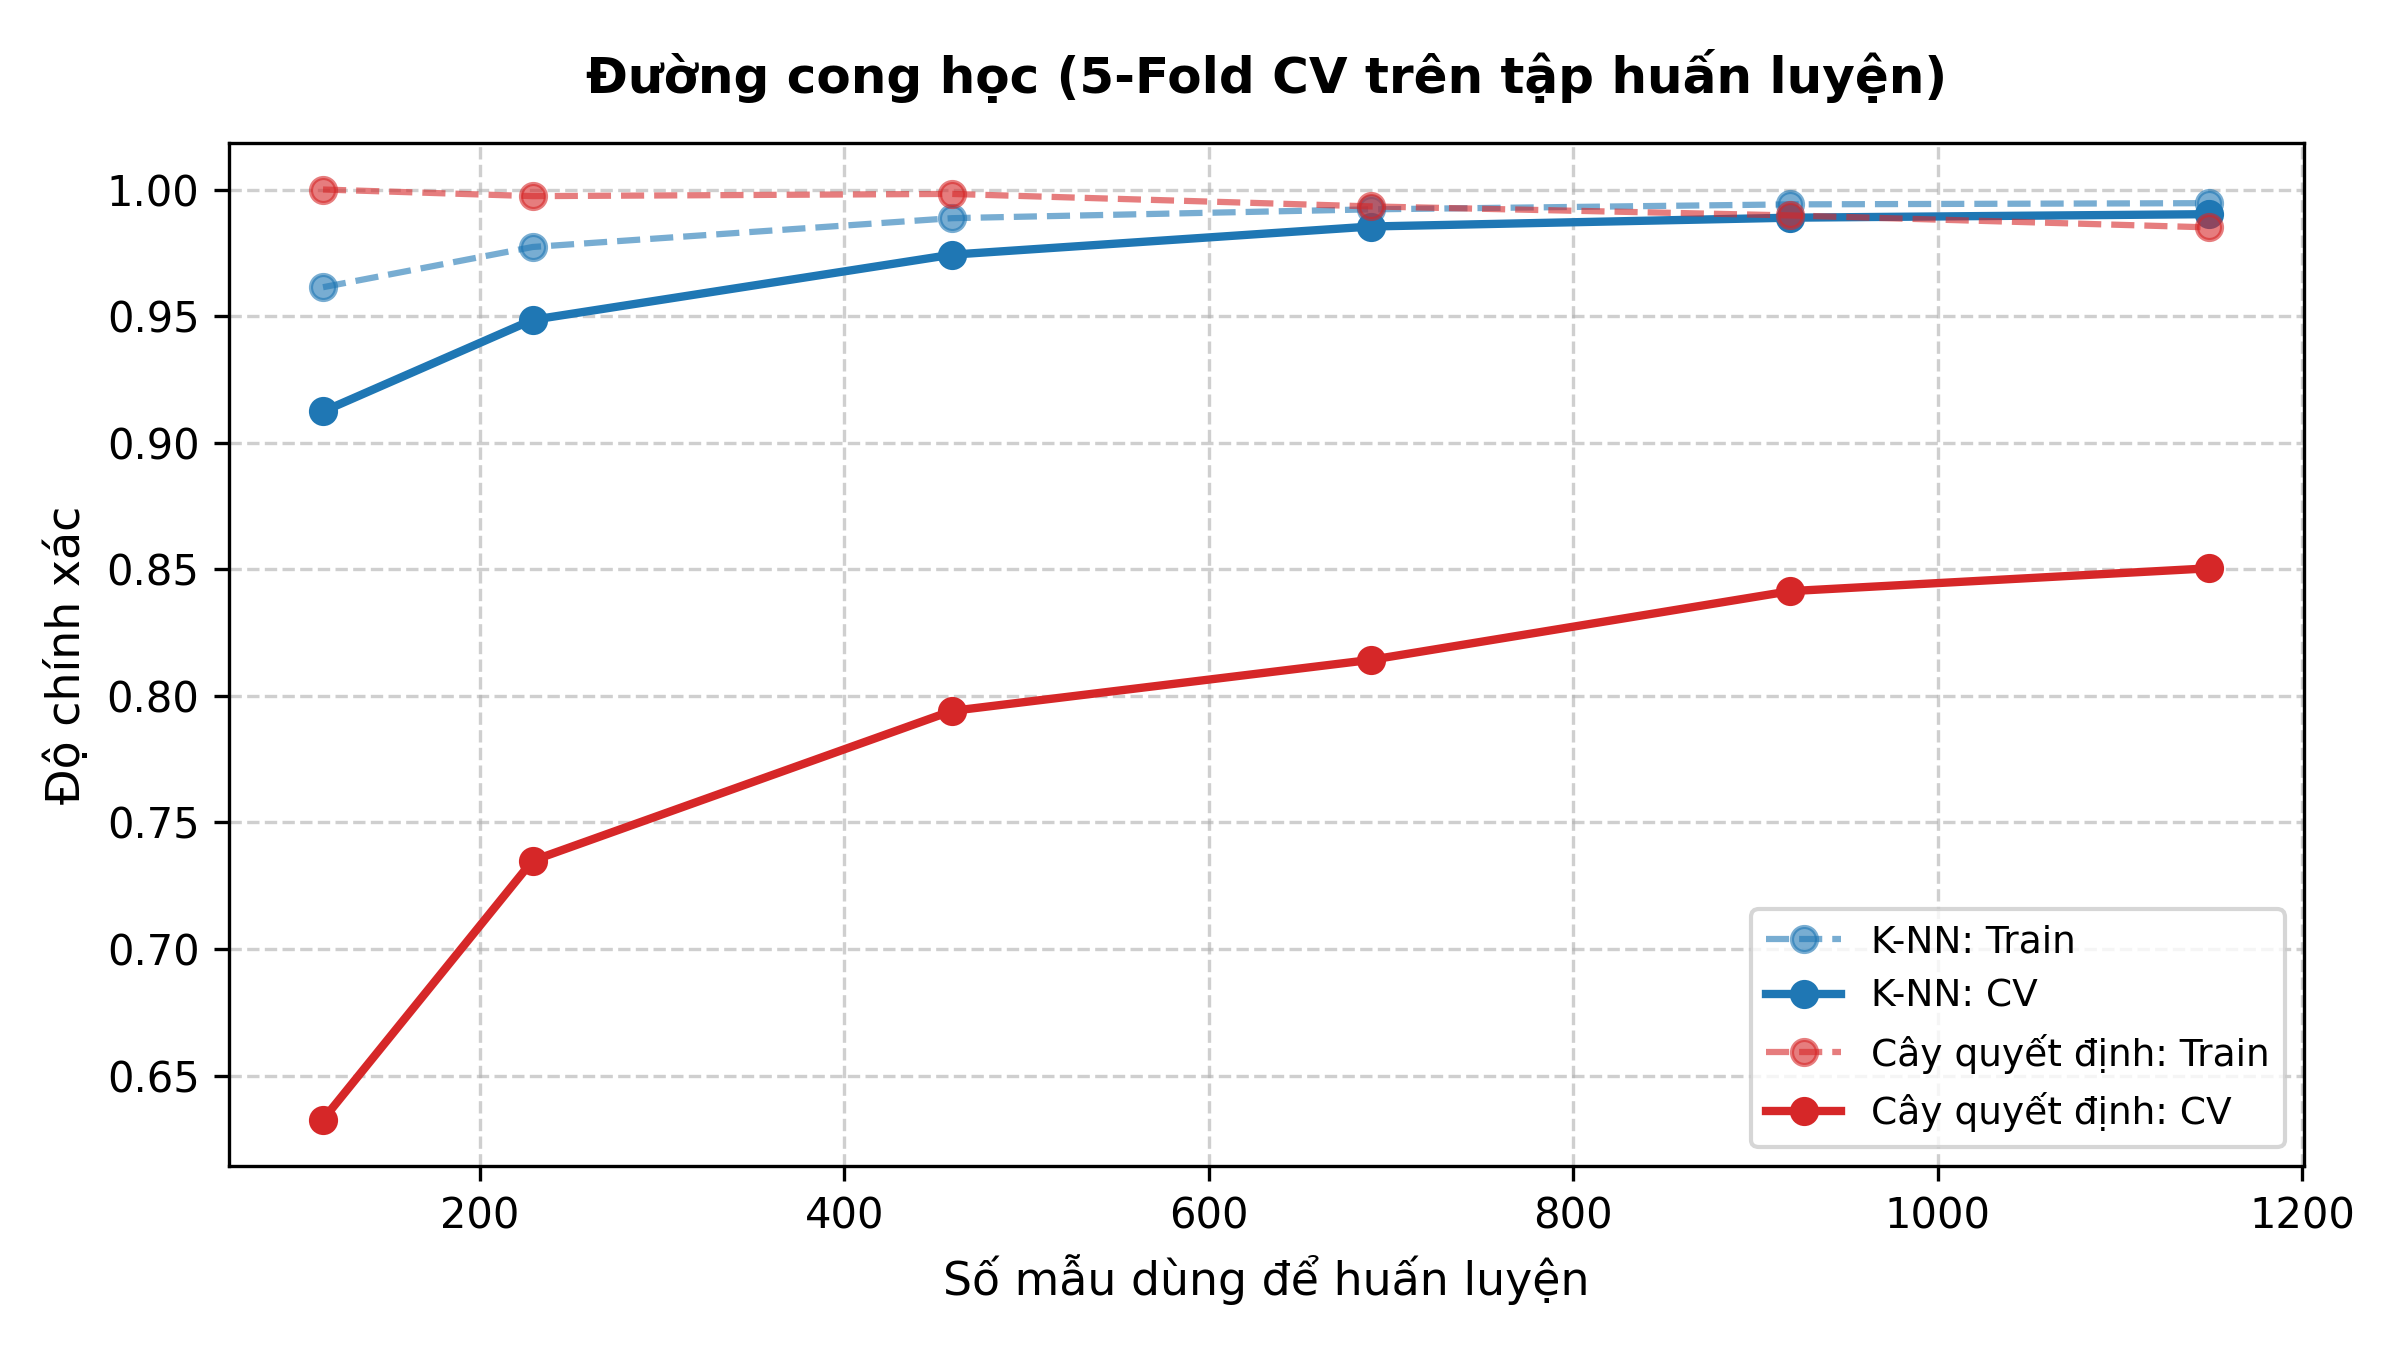
\includegraphics[width=0.75\textwidth]{figures/learning_curve.png}
\caption{Đường cong học của K-NN và cây quyết định}
\label{fig:lc}
\end{figure}

\begin{table}[H]
\centering
\caption{Độ chính xác (\%) theo số mẫu huấn luyện}
\label{tab:lc}
\begin{tabular}{@{}c|cc|cc@{}}
\toprule
\multirow{2}{*}{\textbf{Số mẫu}} & \multicolumn{2}{c|}{\textbf{K-NN}} & \multicolumn{2}{c}{\textbf{Cây quyết định}} \\
 & Train & CV & Train & CV \\
\midrule
\csname @@input\endcsname learning_curve.tex
\bottomrule
\end{tabular}
\end{table}

K-NN đạt 91,23\% chỉ với 114 ảnh huấn luyện và tăng nhanh lên 98,54\% với 689 ảnh, sau đó gần như bão hòa ở 99\%.
Khoảng cách giữa độ chính xác huấn luyện và CV của K-NN chỉ còn 0,43\% khi dùng toàn bộ dữ liệu, tức là mô hình có
phương sai thấp. Ngược lại, cây quyết định luôn đạt gần 100\% trên tập huấn luyện nhưng độ chính xác CV chỉ tăng từ
63,26\% lên 85,04\%, khoảng cách giữa hai đường vẫn còn 13,46\% và đường CV vẫn đang đi lên. Điều này cho thấy cây
quyết định đang bị quá khớp và sẽ còn được cải thiện nếu có thêm dữ liệu, trong khi K-NN đã khai thác gần hết thông
tin của bộ dữ liệu hiện có.

\section{Cấu trúc của cây quyết định}

Cây quyết định tốt nhất có độ sâu 10 và 120 nút lá, tức là trung bình mỗi lá chỉ chứa khoảng 12 ảnh huấn luyện.
Hình~\ref{fig:imp} thể hiện mức độ quan trọng của từng điểm ảnh. Cây chỉ sử dụng 44 trên 64 điểm ảnh; 20 điểm ảnh
còn lại, chủ yếu nằm ở hai cột ngoài cùng và các góc ảnh, không xuất hiện ở bất kỳ nút nào. Điều này khớp với kết
quả thống kê ở Mục 1.4.4: các điểm ảnh ở rìa gần như luôn bằng 0 nên không giúp phân biệt các chữ số. Điểm ảnh quan
trọng nhất nằm ở hàng 2, cột 5 (mức độ quan trọng 0,089), tiếp theo là hàng 4, cột 4 (0,077) và hàng 5, cột 2
(0,073). Các vị trí này nằm ở vùng trung tâm, nơi có thể phân biệt nét cong bên phải của số 2, 3, 9 với nét thẳng
của số 1, 7 hay vòng tròn của số 0, 6, 8.

\begin{figure}[H]
\centering
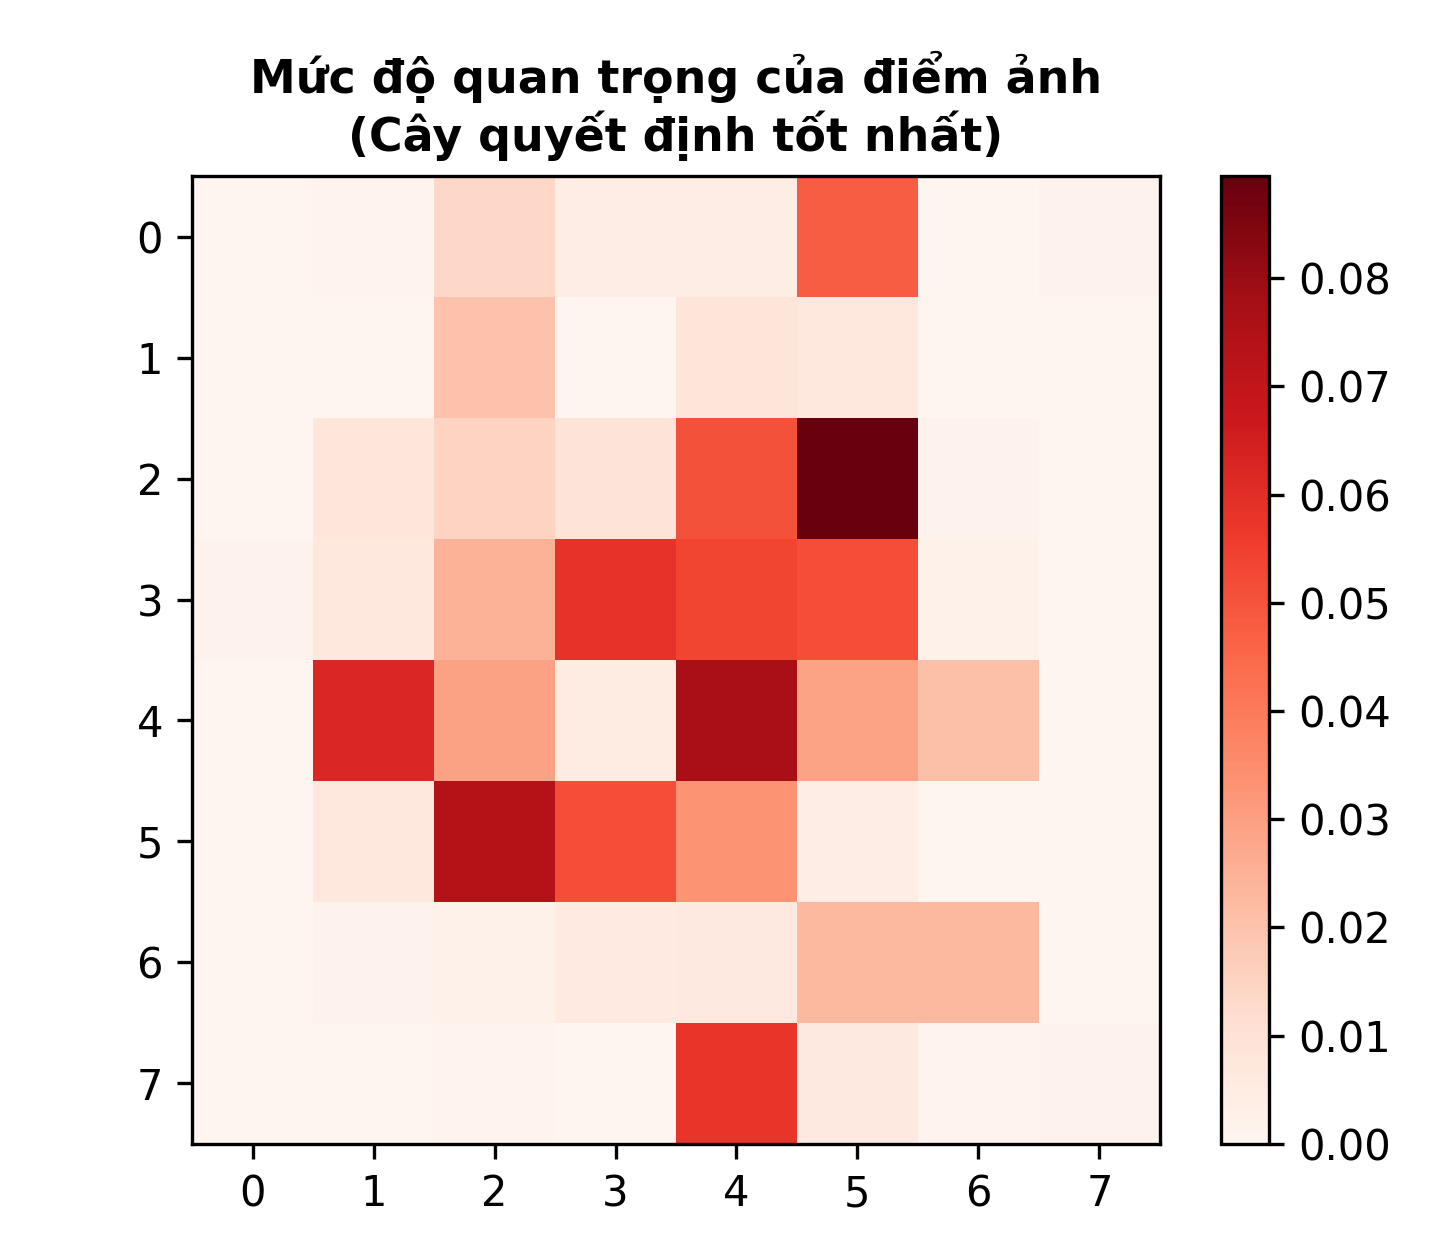
\includegraphics[width=0.5\textwidth]{figures/dt_feature_importance.png}
\caption{Mức độ quan trọng của từng điểm ảnh trong cây quyết định tốt nhất}
\label{fig:imp}
\end{figure}

\section{Kiểm thử ứng dụng demo}
\label{sec:guitest}

\subsection{Kiểm thử định lượng}

Để đánh giá ứng dụng với ảnh nằm ngoài bộ dữ liệu, nhóm dùng tệp \nolinkurl{evaluate_gui_preprocessing.py} tạo ảnh
mô phỏng từ 6 phông chữ với 2 độ dày nét. Có hai loại ảnh: ảnh vẽ trên nền trắng giống vùng vẽ của ứng dụng, và ảnh
chụp giấy có nền xám, ánh sáng không đều, nhiễu và bị mờ nhẹ, kèm theo các biến thể giấy kẻ dòng và có bóng đổ.
Mỗi loại gồm 120 ảnh một chữ số và 60 chuỗi nhiều chữ số (23, 2026, 907, 1458, 36). Một chuỗi chỉ được tính là
đúng khi tất cả các chữ số trong chuỗi đều đúng. Kết quả được trình bày trong Bảng~\ref{tab:gui}.

\begin{table}[H]
\centering
\caption{Kết quả kiểm thử ứng dụng trên ảnh ngoài bộ dữ liệu}
\label{tab:gui}
\begin{tabular}{@{}lcccc@{}}
\toprule
\textbf{Loại ảnh} & \textbf{Một chữ số} & \textbf{Tỉ lệ (\%)} & \textbf{Chuỗi nhiều số} & \textbf{Tỉ lệ (\%)} \\
\midrule
\csname @@input\endcsname gui_eval.tex
\bottomrule
\end{tabular}
\end{table}

Các lựa chọn trong bước tiền xử lý đều được quyết định bằng thực nghiệm trên cùng bộ ảnh mô phỏng này. Với ảnh vẽ
bằng chuột, giữ nguyên độ dày nét cho kết quả tốt hơn so với chuẩn hóa độ dày nét (131 so với 123 trên 160 ảnh
trong thử nghiệm sơ bộ). Với ảnh chụp giấy, chuẩn hóa độ dày nét giúp tăng độ chính xác từ khoảng 78\% lên khoảng
81\%. Với bước tách chữ số, tỉ lệ rộng trên cao 0,85 kết hợp với cắt tại khe hẹp giúp tách đúng số lượng chữ số ở
toàn bộ 60 chuỗi viết cách nhau.

\subsection{Minh họa sử dụng ứng dụng}

Hình~\ref{fig:demo_draw} minh họa trường hợp người dùng vẽ chữ số 5 trên vùng vẽ. Ứng dụng nhận dạng đúng chữ số 5
với độ tin cậy 100\%, tức là cả 3 láng giềng gần nhất đều thuộc lớp 5. Ảnh $8 \times 8$ sau tiền xử lý ở góc dưới
cột giữa cho thấy chữ số đã được đưa về đúng dạng của dữ liệu huấn luyện: nét sáng trên nền tối, chiếm trọn chiều
cao ảnh.

\begin{figure}[H]
\centering
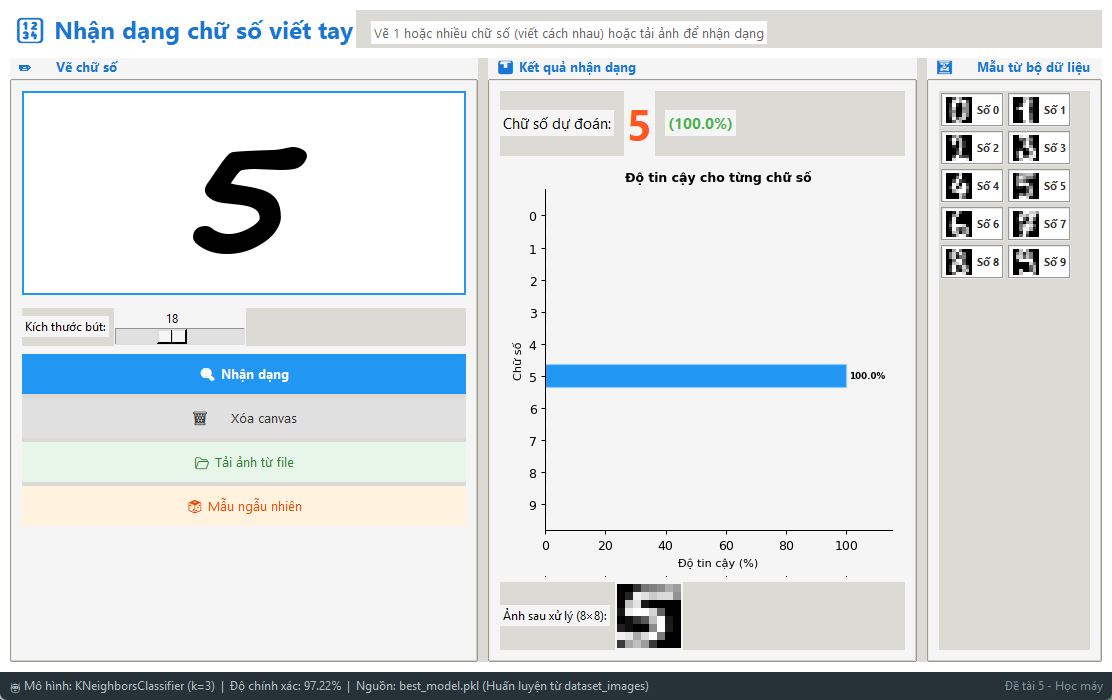
\includegraphics[width=\textwidth]{figures/demo_ve_mot_chu_so.png}
\caption{Nhận dạng chữ số 5 được vẽ trên vùng vẽ của ứng dụng}
\label{fig:demo_draw}
\end{figure}

Hình~\ref{fig:demo_photo} minh họa trường hợp tải lên ảnh chụp chữ số 7 viết trên giấy kẻ dòng, nền xám và ánh sáng
không đều. Sau bước tách nét mực và xóa dòng kẻ, ứng dụng nhận dạng đúng chữ số 7 với độ tin cậy 100\%. Ảnh
$8 \times 8$ sau xử lý không còn dấu vết của các dòng kẻ ngang.

\begin{figure}[H]
\centering
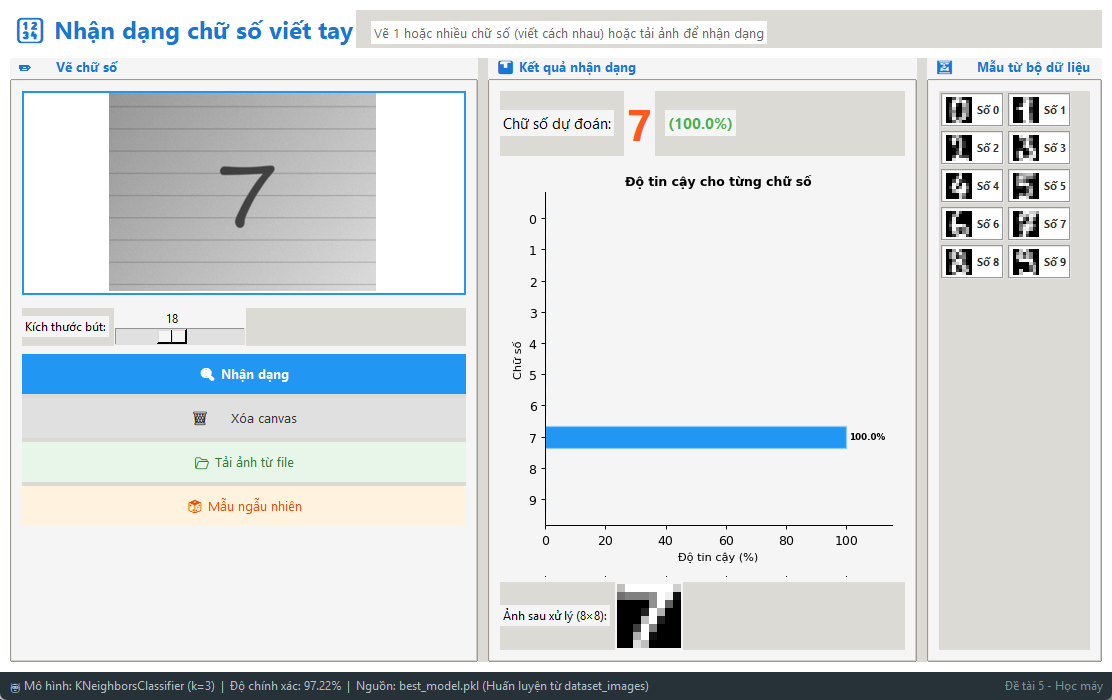
\includegraphics[width=\textwidth]{figures/demo_anh_chup_giay.png}
\caption{Nhận dạng chữ số 7 từ ảnh chụp trên giấy kẻ dòng}
\label{fig:demo_photo}
\end{figure}

Hình~\ref{fig:demo_random} là cửa sổ mẫu ngẫu nhiên, hiển thị 12 ảnh lấy ngẫu nhiên từ tập kiểm thử. Trong lần chạy
này, mô hình dự đoán đúng 11 trên 12 ảnh; ảnh sai là một chữ số 4 bị nhận thành 7, đây cũng là một trong các cặp
nhầm lẫn đã xuất hiện trong phân tích lỗi ở Mục 5.3. Chức năng này giúp người dùng thấy rằng mô hình không hoàn hảo
và hiểu rõ hơn các trường hợp khó.

\begin{figure}[H]
\centering
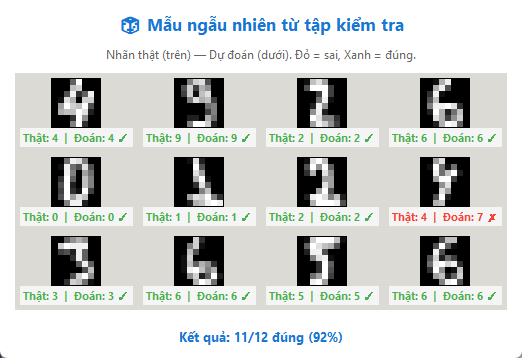
\includegraphics[width=0.62\textwidth]{figures/demo_mau_ngau_nhien.png}
\caption{Cửa sổ dự đoán 12 mẫu ngẫu nhiên từ tập kiểm thử}
\label{fig:demo_random}
\end{figure}

% ======================================================================
\chapter{THẢO LUẬN VÀ SO SÁNH}
% ======================================================================

\section{So sánh K-NN và cây quyết định}

K-NN vượt trội so với cây quyết định với độ chính xác kiểm thử 97,22\% so với 83,89\%. Nguyên nhân là dữ liệu đã
được căn giữa và chuẩn hóa kích thước, nên hai ảnh cùng một chữ số có vector điểm ảnh gần nhau và khoảng cách
Euclid so sánh được đồng thời cả 64 điểm ảnh. Kết quả này xác nhận giả thuyết thứ nhất đã nêu ở Mục 1.4.5. Nhược
điểm của K-NN là phải lưu toàn bộ tập huấn luyện và tính khoảng cách tới mọi mẫu khi dự đoán, với độ phức tạp
$O(N \cdot D)$. Bảng~\ref{tab:results} cho thấy K-NN huấn luyện gần như tức thời (dưới 1 ms) nhưng mất khoảng 15 ms
để dự đoán 360 ảnh, trong khi cây quyết định dự đoán chưa tới 1 ms.

Cây quyết định có ưu điểm là dự đoán nhanh và dễ diễn giải, nhưng mỗi nút chỉ xét một điểm ảnh với một ngưỡng,
nên các ranh giới quyết định đều song song với trục tọa độ. Cách tách này không mô tả được quan hệ giữa các điểm
ảnh lân cận như nét chéo hay đường cong. Ngoài ra, cây dễ bị quá khớp: khi không giới hạn độ sâu, độ chính xác
trên tập huấn luyện đạt 100\% nhưng độ chính xác CV chỉ khoảng 85\%.

Xét theo góc độ độ chệch và phương sai, đường cong học ở Mục 4.5 cho thấy hai mô hình gặp hai vấn đề khác nhau.
K-NN có khoảng cách giữa độ chính xác huấn luyện và CV rất nhỏ (0,43\%), tức là cả độ chệch và phương sai đều thấp
trên bộ dữ liệu này. Cây quyết định có khoảng cách 13,46\%, phương sai cao, nên các biện pháp giảm phương sai như
thêm dữ liệu, giới hạn độ sâu hoặc kết hợp nhiều cây (rừng ngẫu nhiên) sẽ có tác dụng rõ rệt với mô hình này.

So với baseline, cấu hình $k = 3$ cao hơn trên CV (99,03\% so với 98,40\%) nhưng thấp hơn 0,56\% trên tập kiểm
thử, tương ứng 2 trên 360 ảnh. Vì tập kiểm thử nhỏ, chênh lệch này nằm trong mức dao động ngẫu nhiên. Nhóm giữ
nguyên nguyên tắc chọn mô hình theo CV thay vì theo kết quả kiểm thử để tránh đánh giá quá lạc quan. Một lợi thế
nữa của $k = 3$ so với $k = 1$ là mô hình cho ra độ tin cậy có ý nghĩa (tỉ lệ phiếu bầu), được tận dụng trong
khuyến nghị ứng dụng ở Mục~\ref{sec:recommend}.

\section{Ảnh hưởng của biểu diễn đặc trưng}

HOG cho kết quả kém nhất với cả hai thuật toán (91,94\% với K-NN và 77,78\% với cây quyết định), xác nhận giả thuyết
thứ ba. HOG vốn được thiết kế cho ảnh có kích thước lớn; trên ảnh $8 \times 8$, mỗi ô $2 \times 2$ chỉ có 4 điểm ảnh
nên lược đồ 8 hướng rất nhiễu. Bên cạnh đó, HOG bỏ qua cường độ sáng tuyệt đối, vốn là tín hiệu chính của ảnh nhỏ
đã được chuẩn hóa. Với cây quyết định, HOG còn có độ lệch chuẩn CV lớn nhất (3,98\%), cho thấy các đặc trưng này
kém ổn định giữa các fold.

PCA với 28 thành phần giữ được 95\% phương sai, xác nhận giả thuyết thứ hai. Với K-NN, độ chính xác kiểm thử của PCA
là 97,50\%, chênh 1 ảnh so với điểm ảnh thô, trong khi độ chính xác CV thấp hơn một chút (98,89\% so với 99,03\%).
Với cây quyết định, PCA cao hơn điểm ảnh thô trên tập kiểm thử (85,83\% so với 83,89\%) nhưng thấp hơn trên CV
(82,47\% so với 85,04\%). Do hai tiêu chí cho kết luận ngược nhau và chênh lệch nằm trong độ lệch chuẩn của CV, nhóm
đánh giá PCA tương đương điểm ảnh thô về độ chính xác. Về lý thuyết, PCA giảm chi phí tính khoảng cách theo số chiều;
tuy nhiên với tập dữ liệu nhỏ, thời gian dự đoán chỉ thay đổi khoảng 1 ms vì chi phí cố định của thư viện chiếm phần
lớn. Lợi ích về tốc độ và bộ nhớ của PCA sẽ rõ hơn khi dữ liệu lớn.

\section{Phân tích các dự đoán sai}
\label{sec:errors}

\begin{figure}[H]
\centering
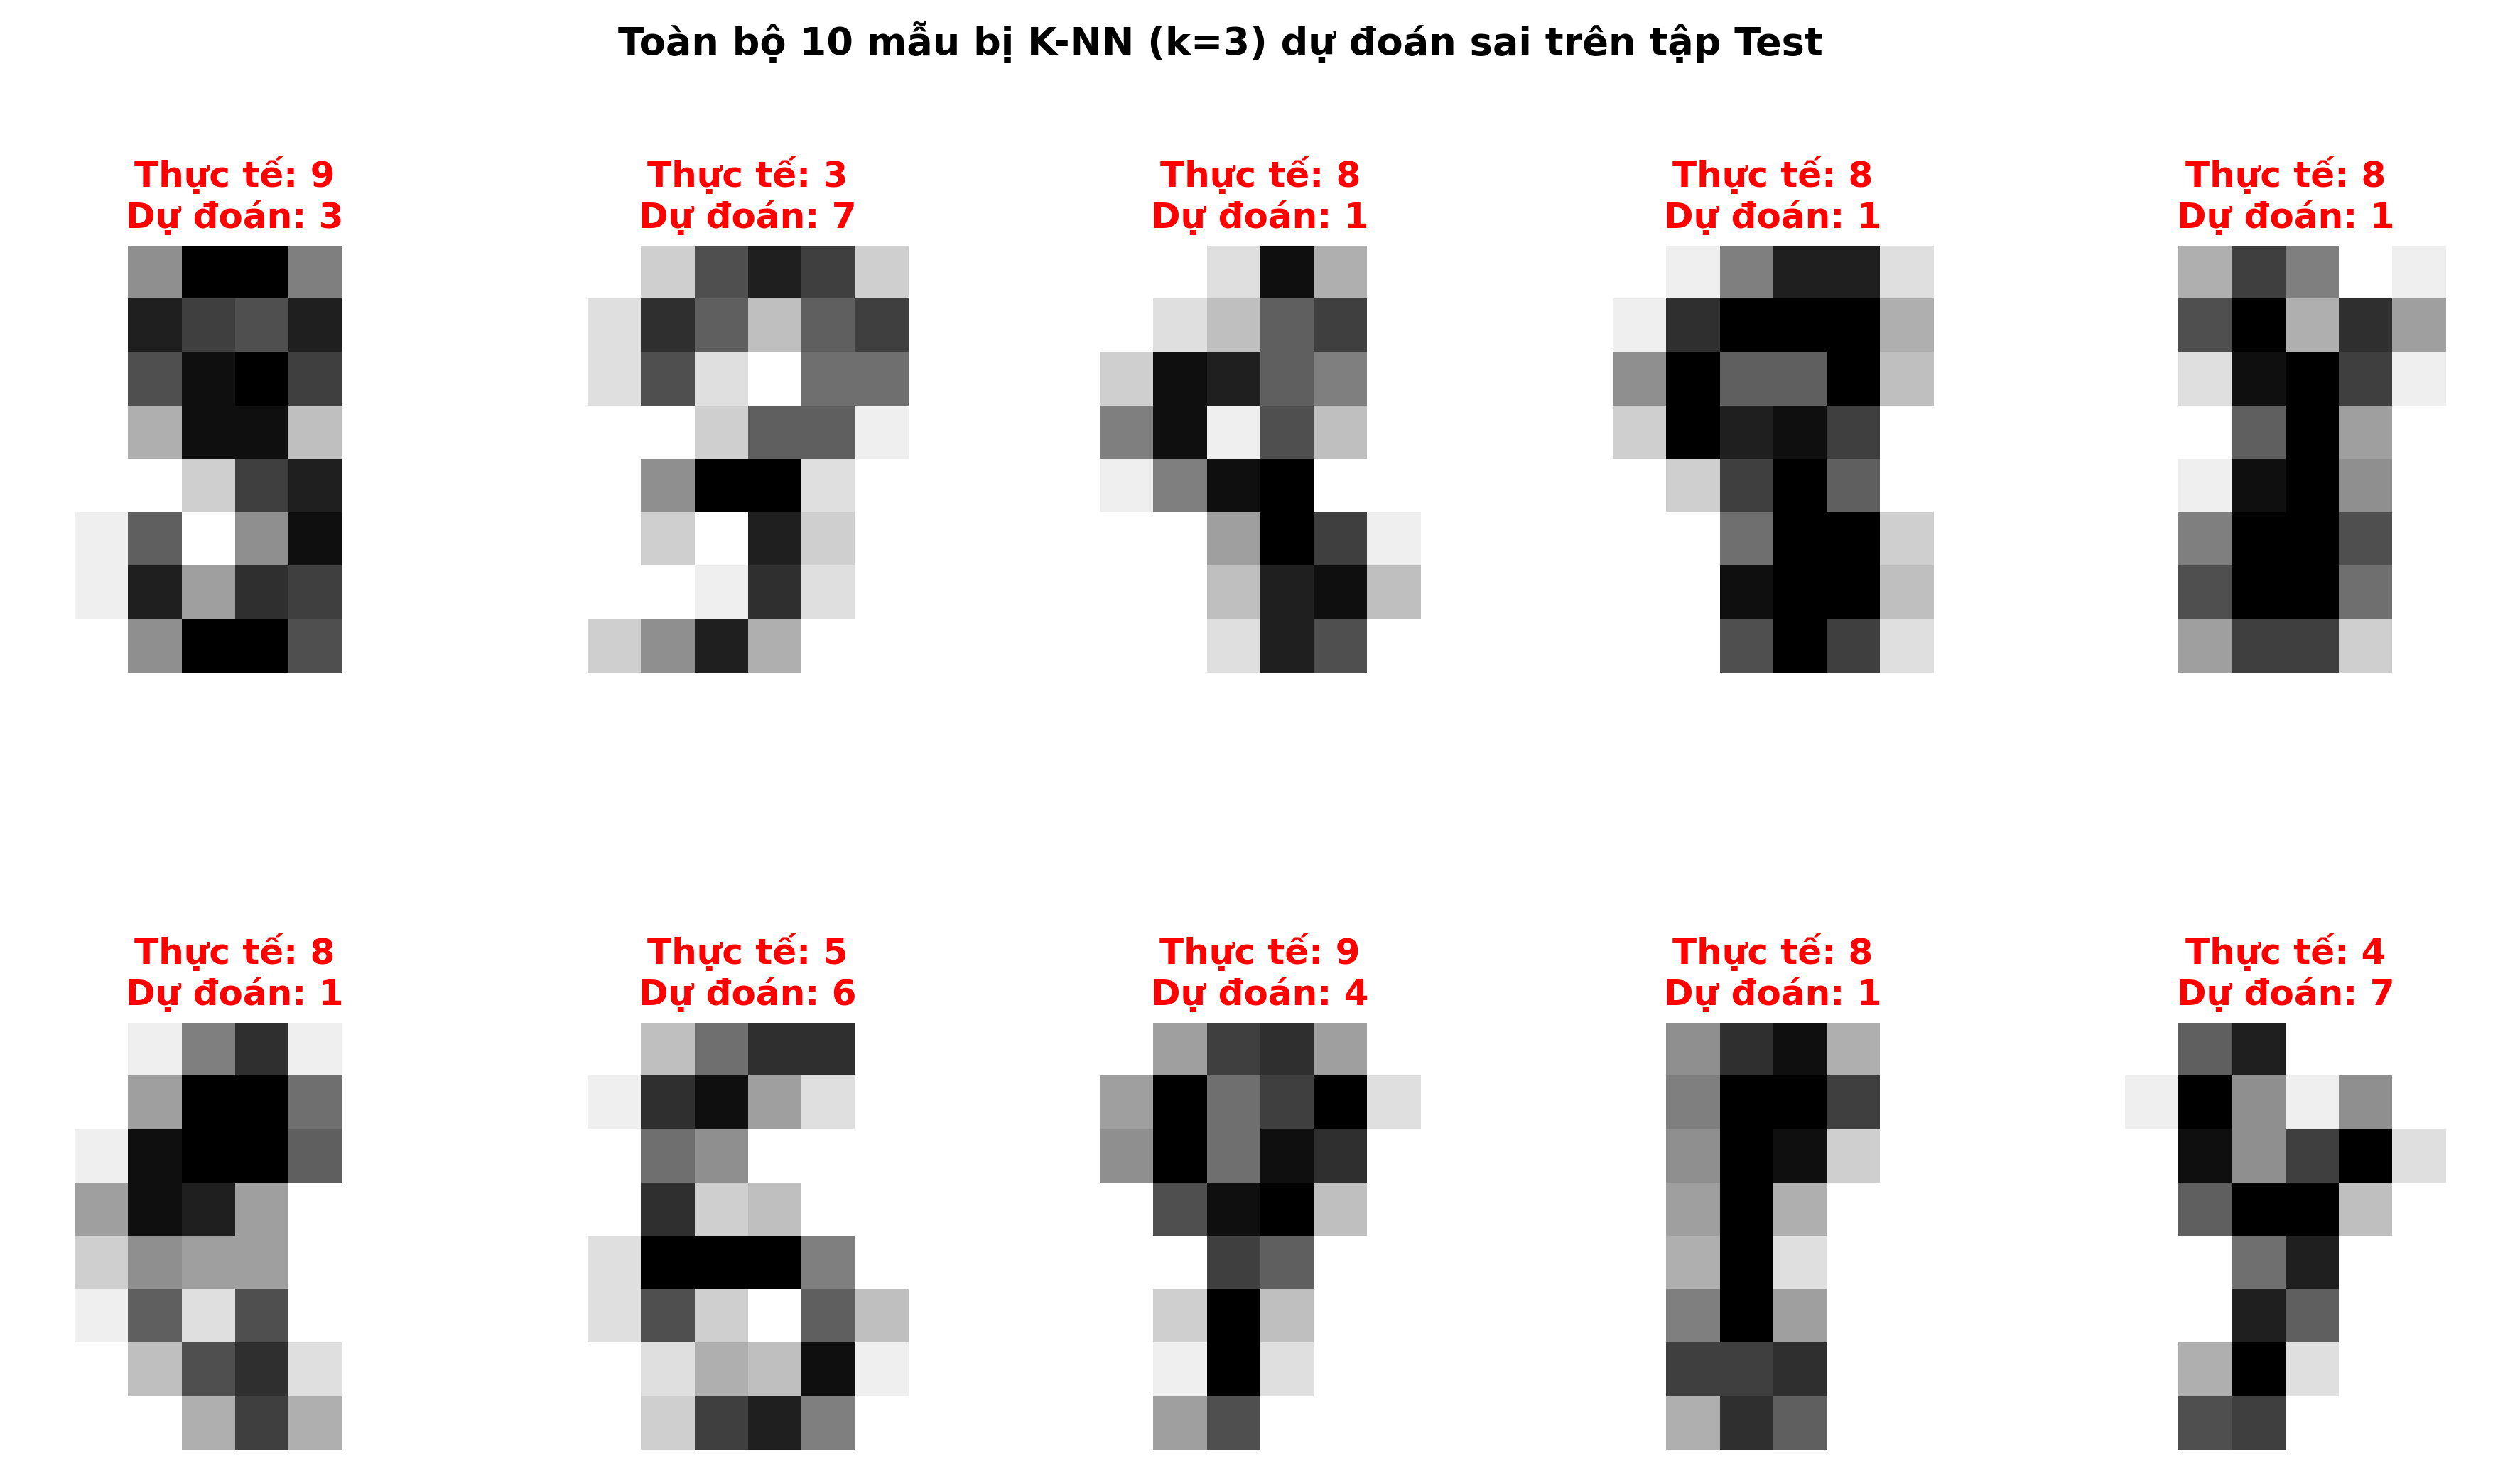
\includegraphics[width=0.92\textwidth]{figures/error_analysis_misclassified.png}
\caption{Toàn bộ các mẫu bị K-NN tốt nhất dự đoán sai trên tập kiểm thử}
\label{fig:errors}
\end{figure}

K-NN tốt nhất dự đoán sai 10 trên 360 ảnh, tương ứng 2,78\% (Hình~\ref{fig:errors}). Lỗi tập trung rõ rệt: 5 trên
10 lỗi là số 8 bị nhận thành số 1, đúng như giả thuyết thứ tư. Quan sát các ảnh này cho thấy số 8 được viết hẹp,
hai vòng bị ép lại, nên sau khi gộp khối $4 \times 4$ chỉ còn một dải sáng thẳng đứng ở giữa, rất giống ảnh trung
bình của số 1. Năm lỗi còn lại là các cặp 3 thành 7, 4 thành 7, 5 thành 6, 9 thành 3 và 9 thành 4, đều là những mẫu
viết lệch hoặc thiếu, thừa nét, chẳng hạn số 9 có vòng trên bị hở giống số 4, hay số 5 có nét dưới khép kín giống
số 6.

Phân tích khoảng cách cho thấy các mẫu bị dự đoán sai thường nằm xa dữ liệu huấn luyện hơn: khoảng cách trung bình
tới láng giềng gần nhất của mẫu sai là 1,31, so với 1,03 của mẫu đúng. Nói cách khác, đây là những cách viết ít gặp
trong tập huấn luyện. Ngoài ra, chỉ 3 trên 10 mẫu sai có cả 3 láng giềng cùng đồng thuận; 7 mẫu còn lại có độ tin
cậy thấp hơn 100\%. Đặc điểm này là cơ sở cho khuyến nghị sử dụng độ tin cậy ở Mục~\ref{sec:recommend}.

Cây quyết định sai 58 trên 360 ảnh. Các cặp nhầm lẫn nhiều nhất được liệt kê trong Bảng~\ref{tab:dtconf}. Cặp 1
thành 9 chiếm nhiều nhất với 7 lỗi, tiếp theo là 3 thành 8 với 5 lỗi. Khác với K-NN, lỗi của cây quyết định phân
tán ở nhiều cặp lớp và không chỉ giới hạn ở các cặp có hình dạng giống nhau, do mỗi quyết định của cây chỉ dựa vào
một vài điểm ảnh riêng lẻ: một nét lệch nhẹ khỏi vị trí quen thuộc có thể đưa mẫu sang một nhánh hoàn toàn khác.

\begin{table}[H]
\centering
\caption{Các cặp nhầm lẫn nhiều nhất của cây quyết định}
\label{tab:dtconf}
\begin{tabular}{@{}cccc@{}}
\toprule
\textbf{Lớp thật} & \textbf{Lớp dự đoán} & \textbf{Số lỗi} & \textbf{Tỉ lệ trên tổng lỗi (\%)} \\
\midrule
\csname @@input\endcsname dt_confusions.tex
\bottomrule
\end{tabular}
\end{table}

Các lỗi này có liên hệ trực tiếp với đặc điểm dữ liệu và giả định của thuật toán. Độ phân giải $8 \times 8$ làm mất
khe hở và vòng khép kín, vốn là chi tiết phân biệt các cặp 8 và 1, 9 và 4, 5 và 6. Đồng thời, K-NN dựa trên cường độ
điểm ảnh tuyệt đối nên không bất biến với độ dày nét và độ rộng của chữ.

\section{Khả năng ứng dụng thực tế}
\label{sec:thucte}

Ở phiên bản đầu, ảnh vẽ tay và ảnh chụp được thu nhỏ trực tiếp về $8 \times 8$ nên khác hẳn dữ liệu huấn luyện;
riêng với ảnh chụp giấy, toàn bộ nền xám bị coi là nét mực. Khi kiểm thử với ảnh chụp mô phỏng, phiên bản này
không nhận đúng ảnh nào trong 120 ảnh. Sau khi bổ sung bước tiền xử lý mô tả ở Mục~\ref{sec:demo}, độ chính xác với
một chữ số đạt khoảng 80\% trở lên ở cả bốn điều kiện trong Bảng~\ref{tab:gui}.

Mức độ chính xác này vẫn thấp hơn rõ rệt so với 97,22\% trên tập kiểm thử. Đây là hiện tượng lệch phân phối dữ
liệu: mô hình chỉ học từ nét chữ của 43 người ở độ phân giải $8 \times 8$, trong khi ảnh thực tế đa dạng hơn nhiều.
Độ chính xác với chuỗi nhiều chữ số thấp hơn nữa vì chuỗi chỉ đúng khi mọi chữ số đều đúng; với xác suất đúng mỗi
chữ số khoảng 0,8, chuỗi bốn chữ số chỉ đúng với xác suất khoảng $0{,}8^4 \approx 0{,}41$. Cần lưu ý rằng ảnh kiểm
thử được tạo từ phông chữ máy tính, nên kết quả chỉ mang tính tham khảo và cần được kiểm chứng thêm trên chữ viết
tay thật của nhiều người.

\section{Khuyến nghị ứng dụng}
\label{sec:recommend}

Trong các ứng dụng thực tế như đọc mã bưu chính hay số tiền trên chứng từ, một lỗi nhận dạng có thể gây hậu quả
lớn hơn nhiều so với việc chuyển một mẫu cho con người kiểm tra lại. Vì vậy, thay vì luôn đưa ra dự đoán, hệ thống
nên chỉ tự động xử lý những mẫu có độ tin cậy cao. Với K-NN $k = 3$, độ tin cậy chính là tỉ lệ láng giềng đồng thuận.
Bảng~\ref{tab:conf} cho thấy kết quả trên tập kiểm thử khi áp dụng các ngưỡng độ tin cậy khác nhau.

\begin{table}[H]
\centering
\caption{Ảnh hưởng của ngưỡng độ tin cậy trên tập kiểm thử}
\label{tab:conf}
\begin{tabularx}{\textwidth}{@{}Lccc@{}}
\toprule
\textbf{Ngưỡng độ tin cậy} & \makecell{\textbf{Số mẫu xử lý}\\\textbf{tự động}} &
\makecell{\textbf{Độ chính xác}\\\textbf{(\%)}} & \makecell{\textbf{Số mẫu chuyển}\\\textbf{kiểm tra}} \\
\midrule
\csname @@input\endcsname knn_confidence.tex
\bottomrule
\end{tabularx}
\end{table}

Khi chỉ tự động xử lý các mẫu có cả 3 láng giềng đồng thuận, hệ thống vẫn xử lý được 96,9\% số mẫu với độ chính xác
tăng từ 97,22\% lên 99,14\%, và chỉ 11 trên 360 mẫu (3,1\%) cần chuyển cho người kiểm tra. Số lỗi giảm từ 10 xuống
còn 3. Đây là cách đánh đổi hợp lý cho các bài toán cần độ chính xác cao.

Ngoài ra, nhóm đưa ra một số khuyến nghị khác khi triển khai. Thứ nhất, ảnh đầu vào cần được chuẩn hóa đúng như dữ
liệu huấn luyện; kết quả ở Mục~\ref{sec:thucte} cho thấy bước tiền xử lý quyết định phần lớn chất lượng nhận dạng
trên ảnh thực tế. Người dùng nên viết chữ số rõ ràng, các chữ số cách nhau, chụp thẳng và đủ sáng. Thứ hai, mô hình
K-NN đã lưu chỉ chiếm khoảng 380 KB và dự đoán một ảnh mất chưa tới 0,1 ms, nên đủ nhẹ để chạy trên máy tính thông
thường hoặc thiết bị nhúng; nếu cần tiết kiệm bộ nhớ hơn, có thể dùng K-NN trên PCA 28 chiều với độ chính xác tương
đương. Thứ ba, khi ứng dụng cho một nhóm người dùng cụ thể, nên thu thập thêm mẫu chữ viết của chính họ để bổ sung
vào tập huấn luyện. Với K-NN, việc này rất đơn giản vì chỉ cần thêm mẫu vào tập dữ liệu mà không cần huấn luyện lại
phức tạp. Cuối cùng, cây quyết định không phù hợp làm mô hình chính cho bài toán này, nhưng có thể dùng trong các
tình huống cần giải thích rõ ràng từng quyết định.

\section{Hạn chế}

Tập dữ liệu nhỏ, chỉ gồm 1.797 ảnh từ 43 người viết và có độ phân giải thấp. Tập kiểm thử chỉ có 360 ảnh nên các
chênh lệch dưới khoảng 1\% giữa các mô hình chưa đủ ý nghĩa thống kê. Cả K-NN và cây quyết định khi làm việc trực
tiếp trên điểm ảnh đều không bất biến với phép xoay, độ dày nét hay kiểu chữ, dẫn đến độ chính xác trên ảnh thực tế
thấp hơn nhiều so với trên tập kiểm thử. Bước tách chữ số trong ứng dụng dựa vào khoảng trống giữa các chữ số,
nên chưa xử lý tốt các chữ số viết dính nhau, chồng lên nhau hoặc viết trên nhiều dòng. Việc kiểm thử ứng dụng
mới dùng ảnh mô phỏng, chưa có bộ ảnh chữ viết tay thật được gán nhãn để đánh giá khách quan.

% ======================================================================
\chapter{TỔNG KẾT VÀ HƯỚNG PHÁT TRIỂN}
% ======================================================================

\section{Kết quả đạt được}

Nhóm đã xây dựng một quy trình học máy hoàn chỉnh và có thể tái lập cho bài toán nhận dạng chữ số viết tay, đọc
trực tiếp dữ liệu từ thư mục ảnh, lựa chọn siêu tham số bằng kiểm định chéo trên tập huấn luyện và chỉ dùng tập
kiểm thử để báo cáo kết quả. Mô hình tốt nhất là K-NN với $k = 3$ và khoảng cách Euclid trên điểm ảnh thô, đạt độ
chính xác CV 99,03\%, độ chính xác kiểm thử 97,22\% và F1 macro 97,20\%, vượt xa cây quyết định (83,89\%). PCA giảm
56\% số chiều mà vẫn giữ được độ chính xác, còn HOG không phù hợp với ảnh $8 \times 8$. Lỗi chủ yếu của mô hình là
nhầm số 8 viết hẹp thành số 1. Ứng dụng demo nhận dạng được một hoặc nhiều chữ số từ ảnh vẽ và ảnh chụp giấy nhờ
bước chuẩn hóa ảnh theo đúng quy trình tạo dữ liệu.

Các phân tích bổ sung giúp hiểu sâu hơn về hai mô hình. Đường cong học cho thấy K-NN đã gần bão hòa với dữ liệu hiện
có, còn cây quyết định bị quá khớp và vẫn có thể cải thiện khi có thêm dữ liệu. Cây quyết định chỉ sử dụng 44 trên
64 điểm ảnh, tập trung ở vùng trung tâm, phù hợp với kết quả thống kê điểm ảnh. Cuối cùng, việc chỉ tự động xử lý
các mẫu mà cả 3 láng giềng đồng thuận giúp nâng độ chính xác của K-NN lên 99,14\% trong khi vẫn xử lý tự động được
96,9\% số mẫu, đây là cách triển khai mà nhóm khuyến nghị cho các ứng dụng thực tế.

\section{Ưu điểm và nhược điểm}

Về ưu điểm, quy trình của nhóm có thể tái lập hoàn toàn nhờ cố định \texttt{random\_state} và tự sinh các bảng số
liệu từ lần chạy thực tế. Siêu tham số được chọn bằng kiểm định chéo trên tập huấn luyện nên kết quả trên tập
kiểm thử phản ánh khách quan khả năng tổng quát hóa. Việc so sánh có hệ thống hai thuật toán trên ba cách biểu diễn
đặc trưng giúp giải thích rõ vì sao K-NN trên điểm ảnh thô phù hợp nhất với bộ dữ liệu này. Mô hình cuối cùng đơn
giản, huấn luyện gần như tức thời mà vẫn đạt độ chính xác 97,22\%. Ứng dụng demo hoạt động được với cả ảnh vẽ bằng
chuột và ảnh chụp chữ viết trên giấy, nhận dạng được một hoặc nhiều chữ số.

Về nhược điểm, mô hình phụ thuộc vào dữ liệu $8 \times 8$ của 43 người viết nên độ chính xác trên ảnh thực tế chỉ
khoảng 80\%. K-NN phải lưu toàn bộ tập huấn luyện và tính khoảng cách tới mọi mẫu, nên sẽ chậm khi dữ liệu lớn.
Bước tách chữ số dựa vào khoảng trống giữa các chữ số nên chưa xử lý tốt chữ số viết dính. Ngoài ra, việc kiểm
thử ứng dụng mới dùng ảnh mô phỏng từ phông chữ máy tính, chưa có bộ ảnh chữ viết tay thật để đánh giá.

\section{Hướng phát triển}

Trong thời gian tới, nhóm dự kiến tăng cường dữ liệu bằng các phép dịch chuyển, co giãn và thay đổi độ dày nét,
đồng thời thu thập thêm ảnh chữ viết tay thật để mô hình hoạt động ổn định hơn trên ảnh thực tế. Nhóm cũng muốn
thử nghiệm với dữ liệu có độ phân giải cao hơn như MNIST ($28 \times 28$) kết hợp HOG với kích thước ô lớn hơn, so
sánh thêm với Naive Bayes, rừng ngẫu nhiên hoặc mạng nơ-ron tích chập, và cải thiện bước tách chữ số bằng phân tích
thành phần liên thông để hỗ trợ chữ số viết dính và viết nhiều dòng.

% ======================================================================
\chapter*{PHÂN CÔNG NHIỆM VỤ}
\addcontentsline{toc}{chapter}{PHÂN CÔNG NHIỆM VỤ}

\begin{table}[H]
\centering
\renewcommand{\arraystretch}{1.3}
\begin{tabularx}{\textwidth}{|c|c|l|L|}
\hline
\textbf{STT} & \textbf{MSV} & \multicolumn{1}{c|}{\textbf{Họ và tên}} & \multicolumn{1}{c|}{\textbf{Nhiệm vụ}} \\ \hline
1 & 1871020396 & Dương Đức Minh    & Tổ chức dữ liệu, khám phá dữ liệu, tiền xử lý và chia tập \\ \hline
2 & 1871020562 & Nguyễn Tiến Thuận & Nhóm trưởng, thiết kế quy trình, K-NN và PCA, quản lý mã nguồn \\ \hline
3 & 1871020335 & Ngô Minh Khôi     & Đặc trưng HOG, cây quyết định, phân tích lỗi \\ \hline
4 & 1871020395 & Nguyễn Nhật Minh  & Ứng dụng demo, trực quan hóa, soạn thảo báo cáo \\ \hline
\end{tabularx}
\end{table}

% ======================================================================
% Tài liệu tham khảo: xếp theo thứ tự trích dẫn, cỡ chữ 12, dòng thứ hai lùi vào 1 cm
\begingroup
\fontsize{12}{17}\selectfont
\begin{thebibliography}{9}
\addcontentsline{toc}{chapter}{DANH MỤC TÀI LIỆU THAM KHẢO}
\bibitem{sklearn} Fabian Pedregosa và cộng sự (2011), ``Scikit-learn: Machine Learning in Python'',
\emph{Journal of Machine Learning Research}, 12, 2825--2830.
\bibitem{uci} Ethem Alpaydin và Cenk Kaynak (1998), \emph{Optical Recognition of Handwritten Digits} [Bộ dữ liệu],
UCI Machine Learning Repository, \url{https://doi.org/10.24432/C50P49}.
\bibitem{hog} Navneet Dalal và Bill Triggs (2005), ``Histograms of Oriented Gradients for Human Detection'',
\emph{IEEE Conference on Computer Vision and Pattern Recognition (CVPR)}, 1, 886--893.
\bibitem{esl} Trevor Hastie, Robert Tibshirani và Jerome Friedman (2009), \emph{The Elements of Statistical
Learning}, Springer, New York.
\bibitem{otsu} Nobuyuki Otsu (1979), ``A Threshold Selection Method from Gray-Level Histograms'', \emph{IEEE
Transactions on Systems, Man, and Cybernetics}, 9 (1), 62--66.
\end{thebibliography}
\endgroup

% ======================================================================
\appendix
\addtocontents{toc}{\protect\renewcommand{\protect\cftchappresnum}{PHỤ LỤC\ }}

\chapter{BẢNG KẾT QUẢ ĐẦY ĐỦ}
\label{app:full}

Bảng~\ref{tab:full} liệt kê kết quả của toàn bộ 31 cấu hình đã chạy. Các giá trị độ đo tính theo phần trăm, thời
gian tính theo mili giây. Với HOG và PCA, nhóm dùng lại tham số tốt nhất theo CV của mỗi thuật toán.

\begin{table}[H]
\centering
\caption{Kết quả toàn bộ các cấu hình thử nghiệm}
\label{tab:full}
\scriptsize
\setlength{\tabcolsep}{3pt}
\begin{tabular}{@{}lllcccccrr@{}}
\toprule
\textbf{Mô hình} & \textbf{Đặc trưng} & \textbf{Tham số} & \textbf{CV (\%)} & \textbf{Acc} & \textbf{Prec} &
\textbf{Rec} & \textbf{F1} & \makecell[b]{\textbf{Huấn}\\\textbf{luyện}} & \makecell[b]{\textbf{Dự}\\\textbf{đoán}} \\
\midrule
\csname @@input\endcsname results_table.tex
\bottomrule
\end{tabular}
\end{table}

\chapter{KHAI BÁO SỬ DỤNG CÔNG CỤ AI}

Theo hướng dẫn của học phần, nhóm khai báo việc sử dụng công cụ AI như sau; nội dung chi tiết được trình bày trong
tệp \nolinkurl{AI_USAGE.md} của kho mã nguồn. Nhóm sử dụng Antigravity AI Assistant và Claude Code (Anthropic) để
được gợi ý cấu trúc mã nguồn và notebook, rà soát lỗi (lỗi cú pháp trong notebook, việc chọn tham số dựa trên tập
kiểm thử, số liệu chưa khớp giữa các tài liệu), cải thiện bước tiền xử lý ảnh của ứng dụng demo và hỗ trợ định
dạng báo cáo. Mọi số liệu trong báo cáo đều được sinh ra bằng cách chạy mã nguồn. Các thành viên đã đọc, kiểm tra
và có thể giải thích toàn bộ quy trình, mã nguồn và kết quả của nhóm.

\end{document}
